\section{第五章\ 飞升入定：将游戏世界部署到云端}
% 张道平


在刚刚结束的第四章中，我们通过引入影子玩家机制消融了地图服务器之间的物理边界，并利用 Raft 共识算法构建了坚不可摧的一致性底座。至此，从单服的并发调度到多服的协同裁决，我们的游戏世界在逻辑层面已经完备，具备了工业级的承载能力、严谨的状态流转契约以及容错恢复机制。这本由无数 Goroutine 和分布式日志编织而成的“统一史书”，在理论上已经能够容纳成千上万名玩家在其中纵横驰骋。

然而，这一切的繁华目前局限于我们开发者的本地回环之中。无论架构多么严谨，代码多么优雅，如果一个系统只能在开发者的个人电脑上运行，那么它仅仅是一个精致的“原型”，而非真正可交付的“产品”。只要开发机断电或休眠，这个宏大的世界便会瞬间停摆。真正的工程化实践，是要摆脱对脆弱本地环境的依赖，将游戏世界连同其运行法则，完整地封装、分发并托管于高可用的云端算力之上。

本章的任务，便是要带大家走出本地环境，通过三个循序渐进的步骤，建立起一套标准化的云端交付体系。
首先，我们要解决“代码在我电脑上能跑，换台机器就报错”的环境不一致的难题。Docker技术是解决这一问题的关键技术，它把游戏程序连同它依赖的所有环境打成一个标准的“包裹”，确保它无论被丢到哪台服务器上，都能像在本地一样稳定运行，这是云计算资源能够“随取随拿”的前提。

其次，我们要解决资源难管理的痛点。当游戏火爆，服务器从 1 台变成 100 台时，靠人工手动启动和维护简直是灾难。Kubernetes（简称 K8s）可以帮助我们，它就像一位拥有三头六臂的“云端指挥官”，可以自动管理成百上千个服务实例，无论是故障重启还是版本更新，都能自动搞定，不会出现技术人员连夜紧急“上线救火”的情况。

最后，我们将解锁系统弹性的能力。游戏流量有高峰也有低谷，高峰期时需要大量服务器来提供稳定服务，但是用户低谷的时候一直开着服务器太浪费电力，借此我们将在K8s的基础上赋予系统“自动伸缩”的智慧，它就像会呼吸一样，能够根据用户的在线数量，及时调整资源策略，真正实现智能化的“按需使用”。这样一来，我们就踏入了所谓的“云原生”领域，让游戏架构真正具备了工业级的弹性。

\subsection{告别“环境地狱”：Docker 容器化封装}

\subsubsection{从“代码交付”到“环境交付”的系统级变革}

在广义的软件工程领域，存在一个困扰了开发者数十年的系统级难题，那就是“开发环境与运行环境的割裂”。这是贯穿于 Web 服务、人工智能、大数据处理等所有软件形态中的普遍痛点。相信每一位工程师都经历过这种绝望时刻：程序在本地开发机上运行如飞，逻辑严密且测试通过，但一旦部署到测试环境或生产服务器，服务却瞬间崩溃，甚至连日志都无法输出。

这种现象被业界戏称为“在我机器上能跑”定律，其背后的本质是软件系统对宿主环境的“隐性依赖”。我们往往天真地以为，软件交付的仅仅是编译好的二进制文件或脚本代码。但从操作系统层面来看，一个进程的正常运行，实则深度耦合于底层的动态链接库（如 glibc）、特定的内核版本、文件系统的目录结构、用户权限配置、乃至系统时区与字符编码等无数个隐性变量。本地的电脑是一个经过长期调优的“温室”，而线上的服务器可能是一个配置极简、甚至版本老旧的“荒野”。当应用程序试图在两个截然不同的系统底座上运行时，这种环境差异就会被无限放大，导致“水土不服”。

对于追求极致性能的游戏服务端、高吞吐的微服务架构或是依赖特定驱动的 AI 模型而言，这种问题尤为致命。如果为了解决兼容性，需要运维人员手动去每一台服务器上安装补丁、同步配置、对齐版本，那么云原生架构所倡导的“弹性伸缩”与“自动化运维”就成了一纸空谈。毕竟，我们无法在几秒钟内为新扩容的一百台服务器手动完成复杂的环境“装修”。

Docker 的横空出世，正是为了从根本上解决这个系统级矛盾。它带来了一场交付模式的革命：将软件交付的标准，从“发一个安装包”升级为了“发一个完整的运行环境”。Docker 的核心思想在于，既然宿主机的环境不可控，那我们就彻底解耦，不再依赖它。通过将代码、运行时、系统工具、依赖库甚至精简的操作系统内核空间统统打包进一个“密封的集装箱”里，Docker 确保了应用无论是在开发者的笔记本上，还是在云端的数据中心里，都运行在完全一致的原子化环境中。

在 Docker 的架构体系中，这种封装被具象化为两个核心概念：镜像（Image）与容器（Container）。我们可以用“类与对象”或“程序与进程”的关系来类比：镜像是一份静态的、只读的系统快照，它完整刻录了软件运行所需的一切环境细节，一旦构建完成即不可篡改；而容器则是这份镜像在宿主机上启动后的动态实例，它是一个被隔离的沙盒进程。要真正掌握这套体系，我们不能只停留在命令行的使用上，接下来我们将深入系统底层，剖析 Docker 是如何通过联合文件系统（UnionFS）、命名空间隔离（Namespace）等核心技术，在保证轻量化的同时，彻底终结“环境地狱”的。

\subsubsection{镜像与容器：模版与实体的关系}
\begin{figure*}[htbp]
    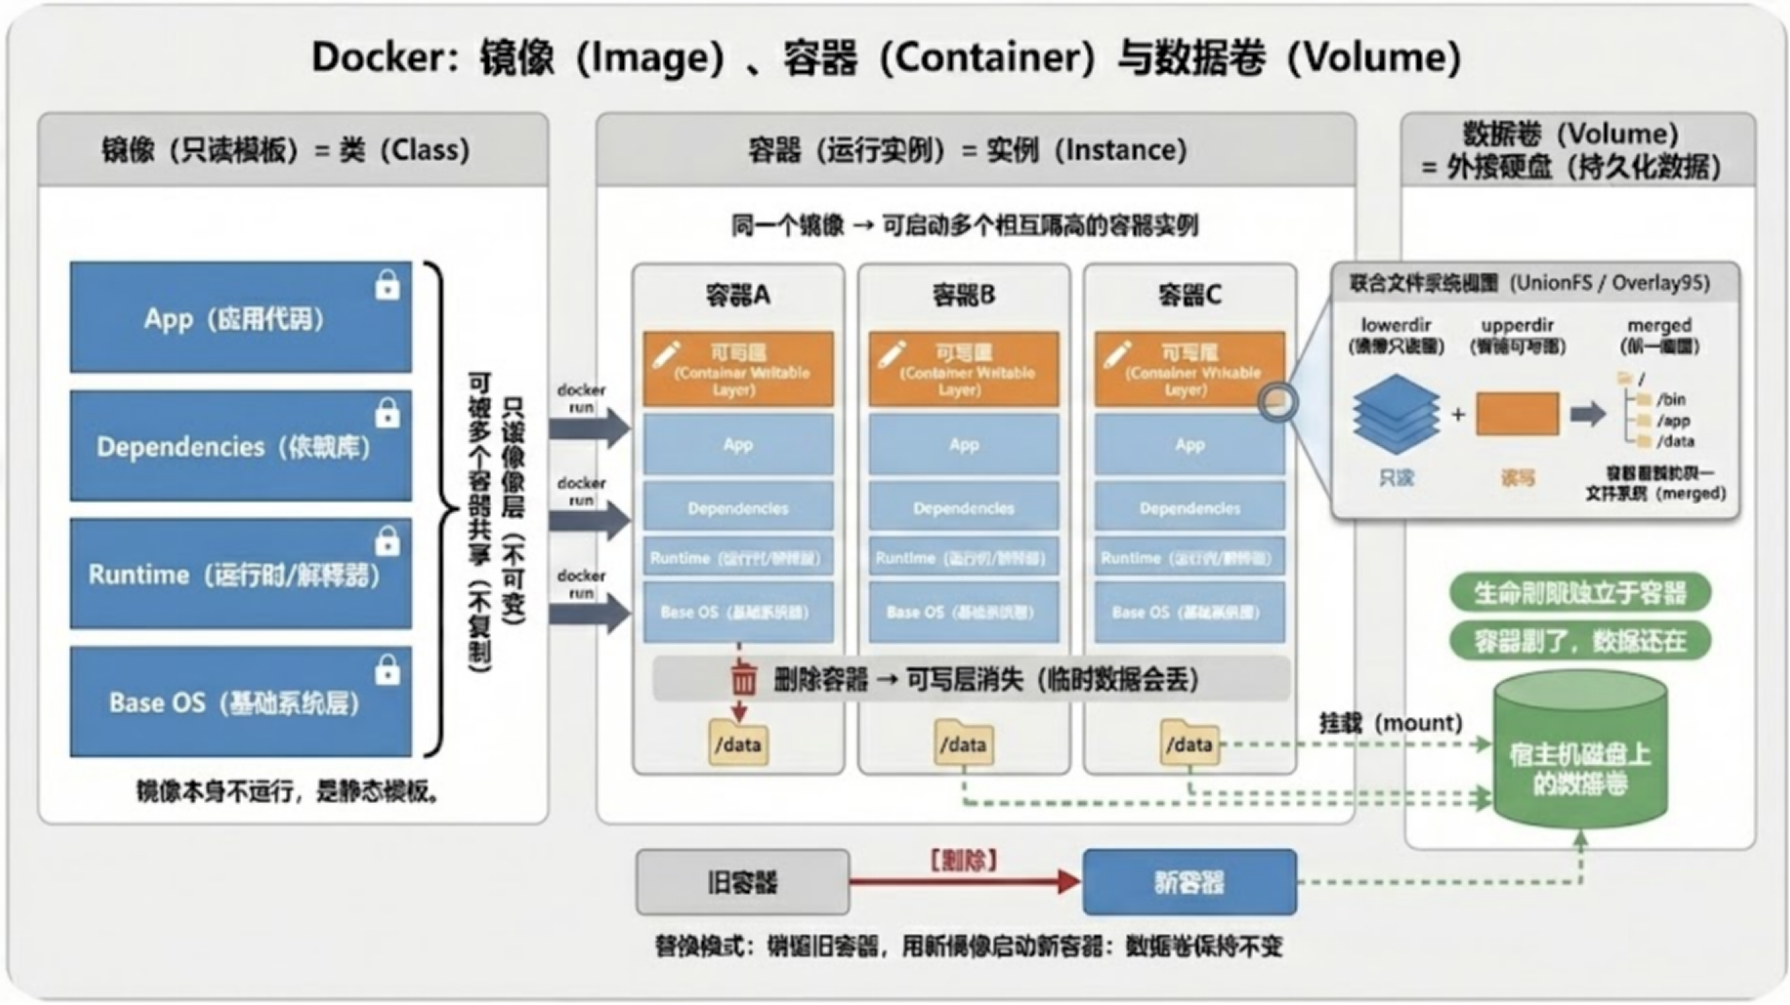
\includegraphics[width=1.0\textwidth]{figures/sec5/chapter5-2.png}
    \caption{镜像、容器以及数据卷}
    \label{fig:chapter5-2}
    \vspace{-15pt}
\end{figure*}


图 \ref{fig:chapter5-2}清晰地展示了 Docker 三大核心概念：镜像、容器与数据卷之间的逻辑关系与生命周期。在 Docker 的概念体系中，“镜像”与“容器”的关系就是图中所示的面向对象编程中的“类”与“实例”。如图左侧所示，镜像是静态的只读模板，它像一个被锁定的“千层饼”，将应用代码、依赖库及基础系统层自下而上封装在一起；而容器则是这个模板在特定宿主机上被“实例化”后的运行现场。正如图片中间部分所示，我们可以基于同一个只读镜像启动容器 A、B、C 等多个实例，它们就像用同一个类 new 出的多个对象，拥有独立的进程空间与网络环境，彼此隔离、互不干扰。这种架构让我们从传统的“修缮模式”彻底转变为图底部的“替换模式”：当应用需要更新时，我们不再修补旧容器，而是直接销毁它，并用新镜像启动新容器，从而保证了环境的绝对纯净。

从系统实现的角度看，容器之所以能做到秒级启动且占用极低，秘密藏在图 \ref{fig:chapter5-2} 中部的联合文件系统（UnionFS）放大视图中。容器并没有复制整个庞大的操作系统，而是采用了“分层复用”的机制：观察图中容器 A、B、C 的内部结构，你会发现它们底部都共享了蓝色的只读镜像层，Docker 仅仅是在这之上挂载了一层可写层。在容器运行期间，程序产生的所有状态变更，无论是写入日志、生成临时缓存，还是修改配置文件，实际上都发生在这个“顶层”里，而底下的镜像层始终保持只读不变。这种机制虽然高效，但也带来了一个必须警惕的副作用：可写层的生命周期是与容器绑定的。正如中下方的流程所示，一旦执行删除容器的操作，这层橙色的可写层也会随之灰飞烟灭，存储在其中的临时数据将永久丢失。

理解了“可写层即易失层”的本质，这就引出了一个棘手的工程问题：如果容器注定是“短命”的，那么像数据库文件、用户上传的图片这些长久的数据该存在哪里？为了解决这个问题，Docker 引入了图 \ref{fig:chapter5-2} 右侧所示的“数据卷（Volume）”。你可以将图中绿色的圆柱体想象成一块插在容器上的“外接硬盘”。通过挂载（mount）操作，我们打通了容器内部路径（如 /data）与宿主机磁盘之间的通道。当程序向这些路径写入数据时，数据流会直接穿透那层易失的橙色可写层，安全地落入宿主机的磁盘中。这样一来，计算逻辑（容器）与业务数据（卷）的生命周期就被彻底解耦了——哪怕你删除了容器、升级了镜像，只要挂载点不变，新启动的服务依然能无缝接管之前的数据，真正实现“铁打的数据，流水的容器”。


\subsubsection{分层构建：将“手工经验”转化为“显性指令”}\label{sec:dockerfile}

\begin{figure*}[htbp]
    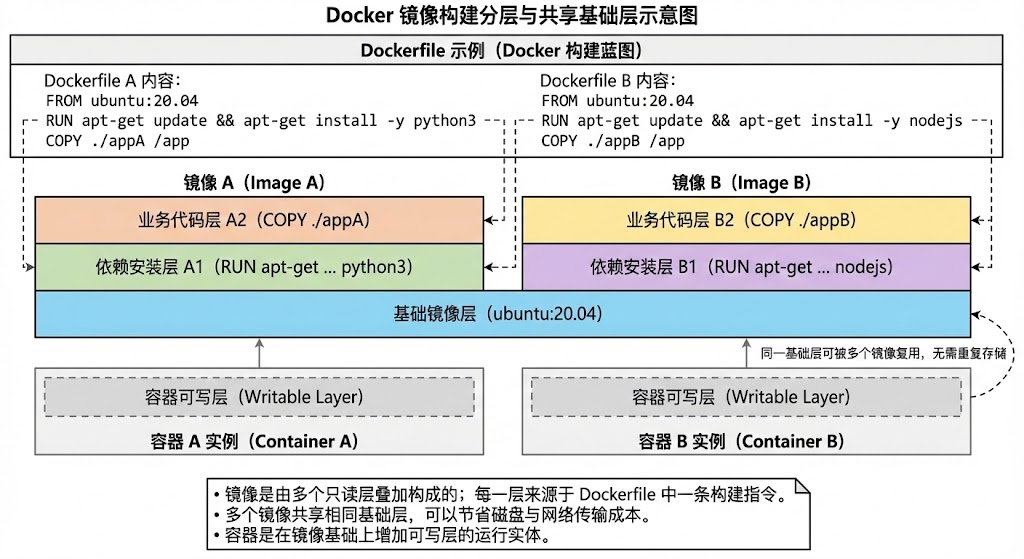
\includegraphics[width=1.0\textwidth]{figures/sec5/chapter5-1.png}
    \caption{Dockerfile构建镜像过程}
    \label{fig:chapter5-1}
    \vspace{-15pt}
\end{figure*}

如图 \ref{fig:chapter5-1} 展示了 Docker 镜像构建的分层机制与共享原理。要确保构建的细节，我们必须理解它是如何被“制造”出来的，Docker 镜像并非一个简单的压缩包，而是严格基于图顶部的 Dockerfile（构建蓝图）生成的。

这份文件充当了不可变的指令集，图中左侧的 Dockerfile A 与右侧的 Dockerfile B 清晰地演示了这一过程：每一行指令都对应一个构建步骤。无论是 FROM 定义的基础环境，还是 RUN 执行的软件安装（如 Python3 或 Node.js），当 Docker 执行这份文件时，会将每一条指令转化为镜像结构中一个独立的只读层。这些层并非混乱堆叠，而是严格按照指令顺序由下至上累积，每一层仅记录相对于上一层发生的增量变化。

这种“指令即图层”的设计在架构层面体现出了显著的优势，首当其冲的便是极致的资源复用。如图中部的蓝色区域所示，虽然镜像 A 与镜像 B 在上层的业务代码与依赖环境上各不相同，但它们均基于 ubuntu:20.04 这一共同的基座。在物理存储层面，这层基础镜像层无需重复冗余，只需存在一份即可被所有上层应用透明共享。这种机制意味着在部署大规模微服务时，系统仅需为各自业务代码（如 appA 或 appB）产生的差异部分“付费”，从而极大地降低了磁盘占用与网络传输的成本。

此外，该设计还实现了确定性与灵活性的完美共存。由于整个构建过程被完全代码化，只要 Dockerfile 保持不变，生成的镜像结构（Image A/B）在任何环境中都能保证分毫不差。如图底部所示当镜像真正投入运行时，Docker 仅需在原有的只读镜像层之上，动态加载一个容器可写层。这一精妙设计既通过只读层保证了底层环境的不可变性，又通过可写层赋予了容器实例必要的运行时读写权限，从而彻底将环境搭建转变为了一条高效、透明且可重复的自动化流水线。

Go 语言常被誉为“云原生时代的 C 语言”，其静态编译特性若能与 Docker 的分层构建机制深度结合，将产生极高的工程价值。纸上得来终觉浅，在上一章中，为了应对多人在线的负载压力，我们将游戏架构垂直拆解为了大厅服务与战斗服务两个独立模块；在本节中我们介绍了Docker的分层构建机制。然而，面对日益增多的服务组件以及未来潜在的水平扩容（如增开一区、二区），倘若机械地为每一个服务单独维护一份 Dockerfile，维护成本无疑将成倍攀升，为此接下来将演示如何编写一份通用的 Dockerfile。

\begin{tcolorbox}[title=拆分后的通用Dockerfile]
\begin{lstlisting}[
    language=bash,
    basicstyle=\ttfamily\footnotesize,
    numbers=left,                   % 开启左侧行号
    numberstyle=\tiny\color{gray},  % 行号样式：灰色小号字体
    numbersep=5pt,                  % 行号与代码的距离
    aboveskip=0pt, belowskip=0pt,
    lineskip=-1pt,
    commentstyle=\color{gray},
    keywordstyle=\color{blue}\bfseries,
    breaklines=true,
    showstringspaces=false
]
FROM golang:1.21-alpine AS builder # 编译环境 
WORKDIR /app # 在容器内的工作目录
COPY go.mod go.sum ./ # 复制关键Go工程文件
RUN go mod download # 下载依赖
COPY . .  # 将源码完整复制
ARG SERVICE # 需要构建的具体服务名
RUN if [ -z "$SERVICE" ]; then echo "ERR: SERVICE not set"; exit 1; fi
# 静态编译：生成的二进制统一命名为 server_bin
RUN CGO_ENABLED=0 GOOS=linux go build -o server_bin ./cmd/${SERVICE}
FROM alpine:latest # 生产环境
RUN apk --no-cache add ca-certificates tzdata # 防止时间偏差
WORKDIR /root/
# 仅从 Builder 阶段复制最终二进制产物与配置
COPY --from=builder /app/server_bin .
COPY --from=builder /app/config ./config
CMD ["./server_bin"]
\end{lstlisting}
\end{tcolorbox}

这份DockerFile就是一张高度标准化的“通用构建蓝图”，核心逻辑采用的就是Docker的“分层多阶段构建”技术，将整个生成流程严谨地划分为“编译”与“运行”两个阶段，旨在解决由于业务扩展导致服务拆分带来的维护难题。

第1-9行是编译阶段，目标是在这里利用完整的工具链将源代码转化为可执行的二进制文件。第1行与第2行事引入包含Go编译器等所有开发工具的官方镜像，它的名字叫做builder，便于后面引用。3-4行是关键优化，我们使用Docker基于文件内容的缓存机制以及Go特有的依赖管理(go.mod)以及安全构建(go.sum)的文件机制来优化编译过程，只要后续go.mod没有引入其他的模块，Docker构建的缓存就会直接跳过下载步骤，这意味着只修改了游戏的逻辑代码时，可以做到“秒级”热启动。当工程依赖构建完成之后才可以把源代码放到容器中，这是由于源代码是改变最频繁的，而Docker的缓存机制是“层层叠加的”，如果移动源代码在构建之前，那么缓存机制就会失效。6-7行是生产者定义针对于传入参数的某种服务构建的分流逻辑，同时避免构建出空壳镜像。第9行则是进行强行静态编译，这意味着生成的可执行文件自带了所有需要的库，不依赖操作系统的动态链接库，这也是为什么容器可以直接部署在极简环境中的原因。

后续则是生产环境，这阶段是“精装修交付”，编译完成后我们会抛弃它们，只保留最终的产品。首先在第10行我们会选择一个极简的底座Alpine，它是一个只有5MB左右的镜像，这好比工厂搭建完工后，我们把起重机、脚手架全部撤走，只留下工厂用于生产了。第11行则是修正时空，容器默认是UTC时间，这是游戏开发中常被忽视的隐患，这里是为了确保服务器能够“读懂”北京时间。14-15行是构建过程的精髓，“from builder”会像一把镊子一样，仅从第一阶段的工厂里夹出编译好的可执行文件以及配置文件，把繁重的源代码以及编译器统统丢弃。最后就是运行可执行文件，这是容器启动时默认执行的命令。

\subsubsection{隔离机制：进程的轻量级虚拟化}

根据上面的描述，我们应该可以发现容器能像虚拟机一样运行服务，但是为什么云计算会使用容器而不是虚拟机？根本原因是它具备业界认可的更轻量？在 图 \ref{fig:chapter5-3} 的宏观对比中，在左侧的传统虚拟机（VM）架构中每一台虚拟机不仅包含应用本身，还必须扛起一套沉重的客体操作系统（Guest OS）与模拟硬件层。这就像为了安顿一位远房亲戚，你得先建造一整栋独立的房子，开销自然极其巨大。反观图示中间的“Docker 容器”架构，你会发现那一层厚重的模拟硬件层和操作系统彻底消失了，取而代之的是所有容器直接坐落在“共享核心内核”之上。这种“进程级隔离”意味着容器不再重复启动内核，省去了漫长的开机自检与繁重的内存损耗，从而实现了“毫秒级启动”与极低资源开销。


那么Docker 是如何让这些共享内核的进程“感觉”自己是在独立运行的呢？答案藏在 图 \ref{fig:chapter5-3} 的右侧面板中，Linux 内核通过两大关键技术为进程构建了隐形的围墙。首先是图右上方的 Namespaces（命名空间），它就像是给进程戴上了一副“特制眼镜”，在 PID（进程号）、NET（网络栈）、MNT（文件挂载点）等维度上构建了独立的视图边界；在容器内部，进程只能看到自己的进程列表和网络接口，完全感知不到宿主机上其他进程的存在。与此同时，图右下方的 Cgroups（控制组） 则扮演了“配额管理员”的角色，它直接对接宿主机的资源池，严格限制了每个容器最多能消耗多少 CPU 时间片和内存大小，防止单个服务因资源失控而将整个服务器拖垮。

\begin{figure*}[htbp]
    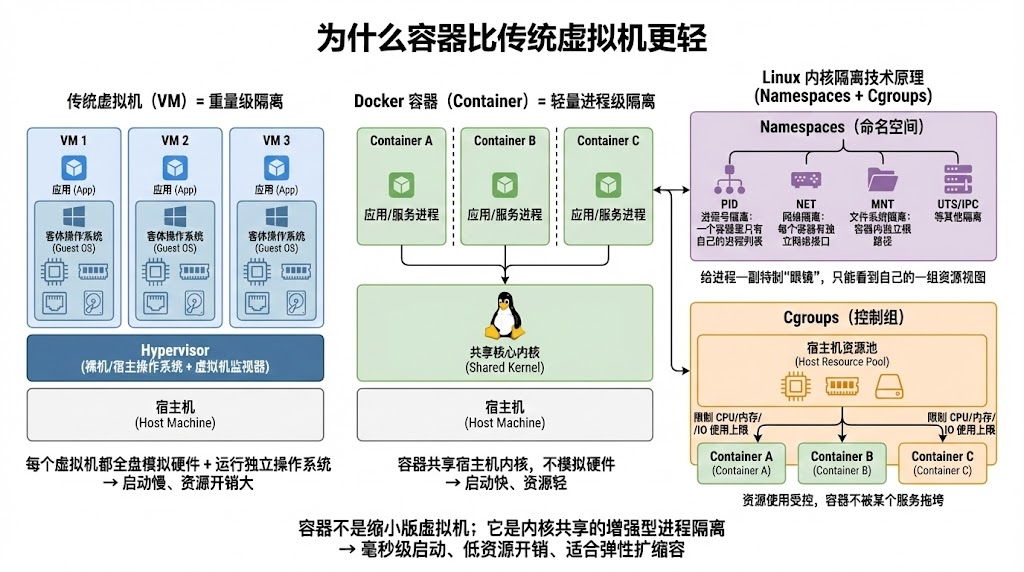
\includegraphics[width=1.0\textwidth]{figures/sec5/chapter5-3.png}
    \caption{容器与虚拟机的对比}
    \label{fig:chapter5-3}
    \vspace{-15pt}
\end{figure*}

理解了这张图的深层逻辑，我们就能建立起对容器最准确的直觉：容器绝不是一个“缩小版的虚拟机”，它的本质是一个“自带隔离边界的增强型进程”。 正是这种“共享内核”与“独占边界”的辩证统一，让 Docker 在保留了隔离安全性的同时，将资源利用率推向了极致。这不仅解释了为何它比虚拟机启动更快，更揭示了它为何能成为微服务架构下实现高频弹性扩缩容的技术基石。


\subsubsection{交付闭环：分发与版本锁定}

\begin{figure*}[htbp]
    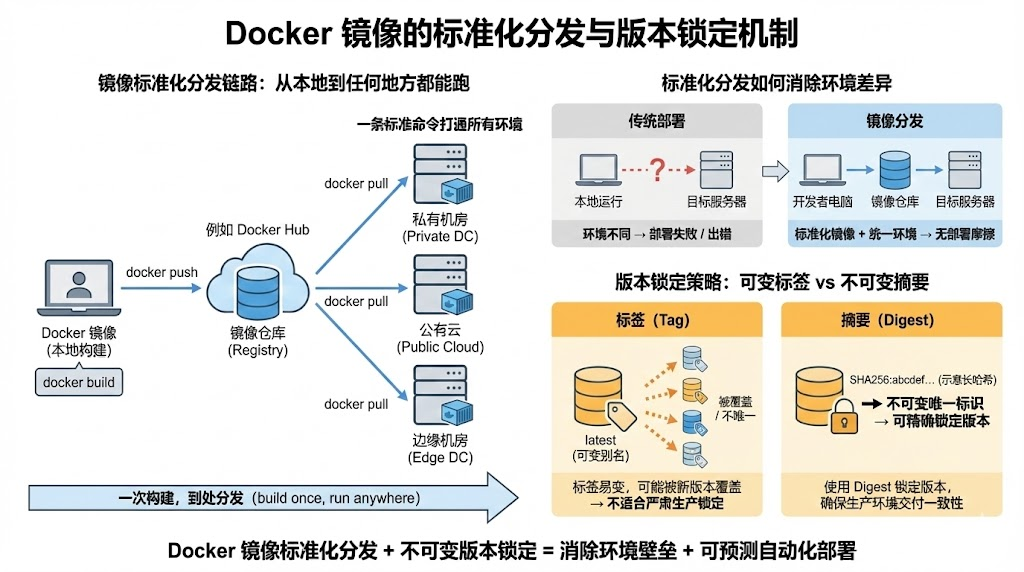
\includegraphics[width=1.0\textwidth]{figures/sec5/chapter5-4.png}
    \caption{Docker的标准化分发链路}
    \label{fig:chapter5-4}
    \vspace{-15pt}
\end{figure*}

Docker 之所以能将“我电脑上能跑”的单点偶然，转化为“处处能跑”的工程必然，其核心不仅取决于容器运行时的隔离性，更依赖于图 \ref{fig:chapter5-4} 所示的标准化分发链路。正如左侧主流程所示，镜像构建完成后，并非孤立存在于开发者的本地机器，而是通过 \texttt{docker push} 指令被推送到远端的镜像仓库（Registry），例如业界通用的 Docker Hub\footnote{Docker Hub: \url{https://hub.docker.com}}。这一机制构建了一个中心化的“软件物流中心”，彻底打通了开发环境与生产环境之间的物理壁垒：无论目标服务器是位于私有机房、公有云还是边缘节点，只要网络连通，运维人员只需执行 \texttt{docker pull} 指令，即可将包含完整运行环境的交付物原样拉取下来。这种“中间库”模式消除了传统部署中点对点拷贝代码导致的“环境摩擦”，真正实现了从“本地运行”到“一次构建，四处分发”的跨越。

为了确保生产环境的绝对严谨，业界在分发环节通常会执行更严格的版本锁定策略，这一关键区别清晰地展示在图 \ref{fig:chapter5-4} 右下角的细节中。虽然 Docker 提供了 \texttt{latest} 等标签（Tag）机制，但标签本质上是可变的别名，极易被新推送的版本覆盖，导致不同时间拉取的 \texttt{latest} 实际上是完全不同的代码。因此，在工程实践中，我们更倾向于使用镜像摘要（Digest）——即对镜像内容进行 SHA256 哈希计算生成的唯一且不可变的标识符——来锁定版本。这标志着软件交付模式的根本性变革：我们将交付过程从传统的“拷贝代码 + 祈祷不报错”，进化为“拉取标准化构件 + 校验唯一哈希 + 按约定启动”。这种基于密码学保证的一致性，使得规模化的自动化部署不再是碰运气的冒险，而是可预测的工程行为。

理论为我们指明了方向，而终端命令则是走完这“发布最后一公里”的具体载体。当我们的战斗服业务代码编写完毕，并按照 \ref{sec:dockerfile} 节的要求定义好 Dockerfile 后，整个交付流水线便正式启动：首先，使用 \texttt{docker build} 命令配合 \texttt{-t} 参数构建出带有版本号的本地镜像；紧接着，通过 \texttt{docker login} 指令与 Docker Hub 或私有仓库建立加密的安全连接，完成身份认证；随后，利用 \texttt{docker tag} 给本地镜像打上带有云端用户名的“发件人标签”，确保其能被准确路由至指定仓库；最后，执行 \texttt{docker push} 将镜像推向云端。在此过程中，Docker 的智能分层机制会确保只上传云端缺失的增量层，极大节省带宽，而推送结束时返回的那串 SHA256 摘要，正是我们在后续 \texttt{pull} 指令中进行精确版本锁定的唯一凭证。

\begin{tcolorbox}[title=镜像发布与版本锁定实操]
\begin{lstlisting}[
    language=bash,
    basicstyle=\ttfamily\footnotesize,
    numbers=left,                   % 开启左侧行号
    numberstyle=\tiny\color{gray},  % 行号样式：灰色小号字体
    numbersep=5pt,                  % 行号与代码的距离
    aboveskip=0pt, belowskip=0pt,
    lineskip=-1pt,
    commentstyle=\color{gray},
    keywordstyle=\color{blue}\bfseries,
    breaklines=true,
    showstringspaces=false
]
docker build -t game-lobby:v1 . # 构建镜像
docker login # 登录镜像仓库
docker tag game-lobby:v1 username/game-lobby:v1 # 打标签
docker push username/game-lobby:v1 # 推送到云端
docker pull username/game-lobby@sha256:[sha256] # 从云端拉取
docker images --digests # 验证镜像是否一致 
\end{lstlisting}
\end{tcolorbox}


然而，掌握了单个容器的标准化交付仅仅是构建云原生架构的起点。现实中的现代应用，尤其是复杂的分布式游戏后端，往往是由多个相互依赖的服务（如游戏服、数据库、缓存、网关）共同构成的有机体。在下一节，我们将把视角从“单机容器”扩展至“集群编排”：利用 Docker Compose 解决多服务协同与本地联调的难题。



\subsection{一键开服：使用 Compose 编排你的游戏``大区''}

\subsubsection{从手工拼装到一键编排}

在上一节中,我们已经掌握了将单个服务封装成 Docker 容器的技能,但现实中的游戏后端绝非孤立的单体应用。回想第四章构建的分布式架构:我们有负责玩家接入的网关服务、处理具体战斗逻辑的地图服务、存储玩家数据的 Redis 缓存,以及记录操作日志的数据库服务。要让这个完整的``游戏大区''真正跑起来,我们需要协调启动至少 5 个不同的容器,并且必须保证它们之间的启动顺序、网络连接和配置传递都恰到好处。

\begin{figure}[htbp]
\centering

\includegraphics[width=0.85\textwidth]{figures/sec5/Docker_Compose_concepts.png}
\caption{Docker Compose 服务编排的核心概念与工作机制}
\label{fig:compose-concepts}
\end{figure}

如图 \ref{fig:compose-concepts} 左上角所示,如果依赖手工操作,这个过程会是一场噩梦。你需要先启动数据库容器,等它完全就绪后再启动 Redis,接着启动地图服务并配置好数据库连接,然后启动网关服务并告诉它地图服务的地址,最后还要确保各个服务的端口不冲突、网络能互通。每次部署都要重复这套繁琐的``开机仪式'',不仅效率低下,更容易在某个环节出错导致整个大区瘫痪。

Docker Compose 的出现正是为了将这种``手工拼装''升级为``一键编排''。如图 \ref{fig:compose-concepts} 右上方所示,它的核心思想是用一份声明式的配置文件来描述整个应用栈的结构,包括每个服务使用哪个镜像、需要暴露哪些端口、依赖哪些其他服务,以及如何进行网络通信。有了这份``施工图纸'',我们只需要执行一条启动命令,Compose 就能自动按照依赖关系的拓扑顺序,将所有容器按部就班地启动起来,并为它们建立好通信网络。这种转变意味着复杂的分布式系统部署从``人工部署''变成了``标准化工序''。

\subsubsection{理解 Docker Compose:从``单兵作战''到``团队协作''}

Docker Compose 本质上是一个容器编排工具,它通过 YAML 格式的配置文件来定义和管理多容器应用。如果说 Docker 解决的是``如何标准化打包单个服务''的问题,那么 Compose 解决的就是``如何协调多个服务共同工作''的问题。

Compose 的工作原理可以类比为指挥一个交响乐团。每个容器就像一个乐器,单独演奏时可能悦耳动听,但要产生和谐的整体效果,就需要指挥家(Compose)来协调各乐器的演奏时机、音量配合和节拍同步。Compose 通过声明式配置,让我们只需要描述``想要什么样的最终效果''(哪些服务需要运行、它们之间如何通信),而无需关心``如何具体实现''(启动命令的顺序、网络配置的细节)。

这种抽象带来的最大价值在于可重现性和可维护性。无论是在开发环境、测试环境还是生产环境,同一份 Compose 配置都能保证部署结果的一致性。当需要新增服务或修改配置时,我们只需要更新配置文件,而不用担心遗漏某个手工步骤导致的环境差异。

\subsubsection{服务分层:构建清晰的架构蓝图}

要编写一份清晰易维护的 Compose 配置,首先需要理解我们的游戏后端中每个服务的职责边界。基于第四章的架构设计,我们可以将整个系统划分为三个核心层次。

如图 \ref{fig:compose-concepts} 右上角的三层架构设计原理图所示,\textbf{数据存储层}作为整个架构的基础,承载着系统的数据持久化职责。Redis 在这一层扮演高速缓存的角色,负责存储玩家的实时状态、会话信息和频繁访问的热点数据;PostgreSQL 作为主数据库,持久化保存玩家账号、装备道具、游戏进度等需要长期保存的核心数据。这两个服务构成了数据层的``双核心'',为上层业务提供快速访问和可靠存储的能力。

\textbf{业务逻辑层}是游戏世界的运算核心,地图服务器在这里承担着最关键的角色。它需要处理玩家的移动、战斗、交易等各种游戏逻辑,同时要与数据层保持密切交互——从 Redis 读取玩家状态、向 PostgreSQL 写入变更记录。地图服务器本质上是一个``数据处理引擎'',它将底层的数据存储转化为上层可理解的业务逻辑。

\textbf{接入控制层}位于整个架构的最顶端,网关服务在这里发挥着``交通枢纽''的作用。它负责接收来自玩家客户端的各种请求,进行身份验证、请求路由、负载均衡等处理,然后将处理过的请求转发给具体的业务服务。网关服务相当于整个游戏后端的``前台接待'',是外部世界与内部业务逻辑之间的桥梁。

这种分层设计的优势在于每一层都有明确的职责边界,服务间的依赖关系呈现出清晰的``自下而上''特征。数据层为业务层提供支撑,业务层为接入层提供服务,形成了稳定的依赖链条。这种设计既保证了系统的稳定性,也为后续的扩展和优化奠定了良好基础。

\subsubsection{依赖编排:破解``先有鸡还是先有蛋''的难题}

在微服务架构中,服务间往往存在明确的依赖关系,这些依赖关系直接决定了服务的启动顺序。地图服务必须等数据库完全启动并准备好接受连接后才能正常工作;网关服务必须在地图服务就绪后才能开始路由请求。如果启动顺序错乱,轻则导致服务启动失败,重则引发级联故障,整个游戏大区都可能因此瘫痪。

Compose 通过依赖声明机制彻底解决了这一问题,它允许我们在配置中明确表达``谁依赖谁''的关系,然后自动计算出正确的启动顺序。如图 \ref{fig:compose-concepts} 左下角所示,通过配置文件中的依赖关系声明,系统可以自动判断启动顺序:数据层服务优先启动,业务层服务等待数据层就绪,接入层服务最后启动。

但是,简单的启动顺序控制还不够。虽然 Compose 能保证 PostgreSQL 容器在地图服务之前启动,但不能保证数据库服务完全可用后再启动地图服务。这就需要引入``健康检查''机制——通过定期检测服务的关键功能是否正常,来判断服务是否真正``就绪''。

如图 \ref{fig:compose-concepts} 左下方的故障编排与健康检查机制示意图所示,健康检查的工作原理类似于医生给病人量体温。系统会定期(如每 30 秒)向服务的特定端点发起检查请求,只有当服务能够正确响应时,才被标记为``健康''状态。对于数据库服务,健康检查可能是尝试执行一个简单的查询;对于 Web 服务,可能是访问一个专门的健康检查接口。只有当所有被依赖的服务都通过健康检查后,依赖它们的服务才会被启动。如果服务异常,系统会进行重试(如 3 次),确保启动的可靠性。

这种``等待就绪''的机制确保了服务启动的可靠性。即使某个服务启动较慢,下游服务也会耐心等待,避免了因为时机不当导致的连接失败。同时,如果某个服务在运行过程中出现问题,健康检查机制也能及时发现并触发相应的恢复措施。

\begin{figure}[htbp]
\centering
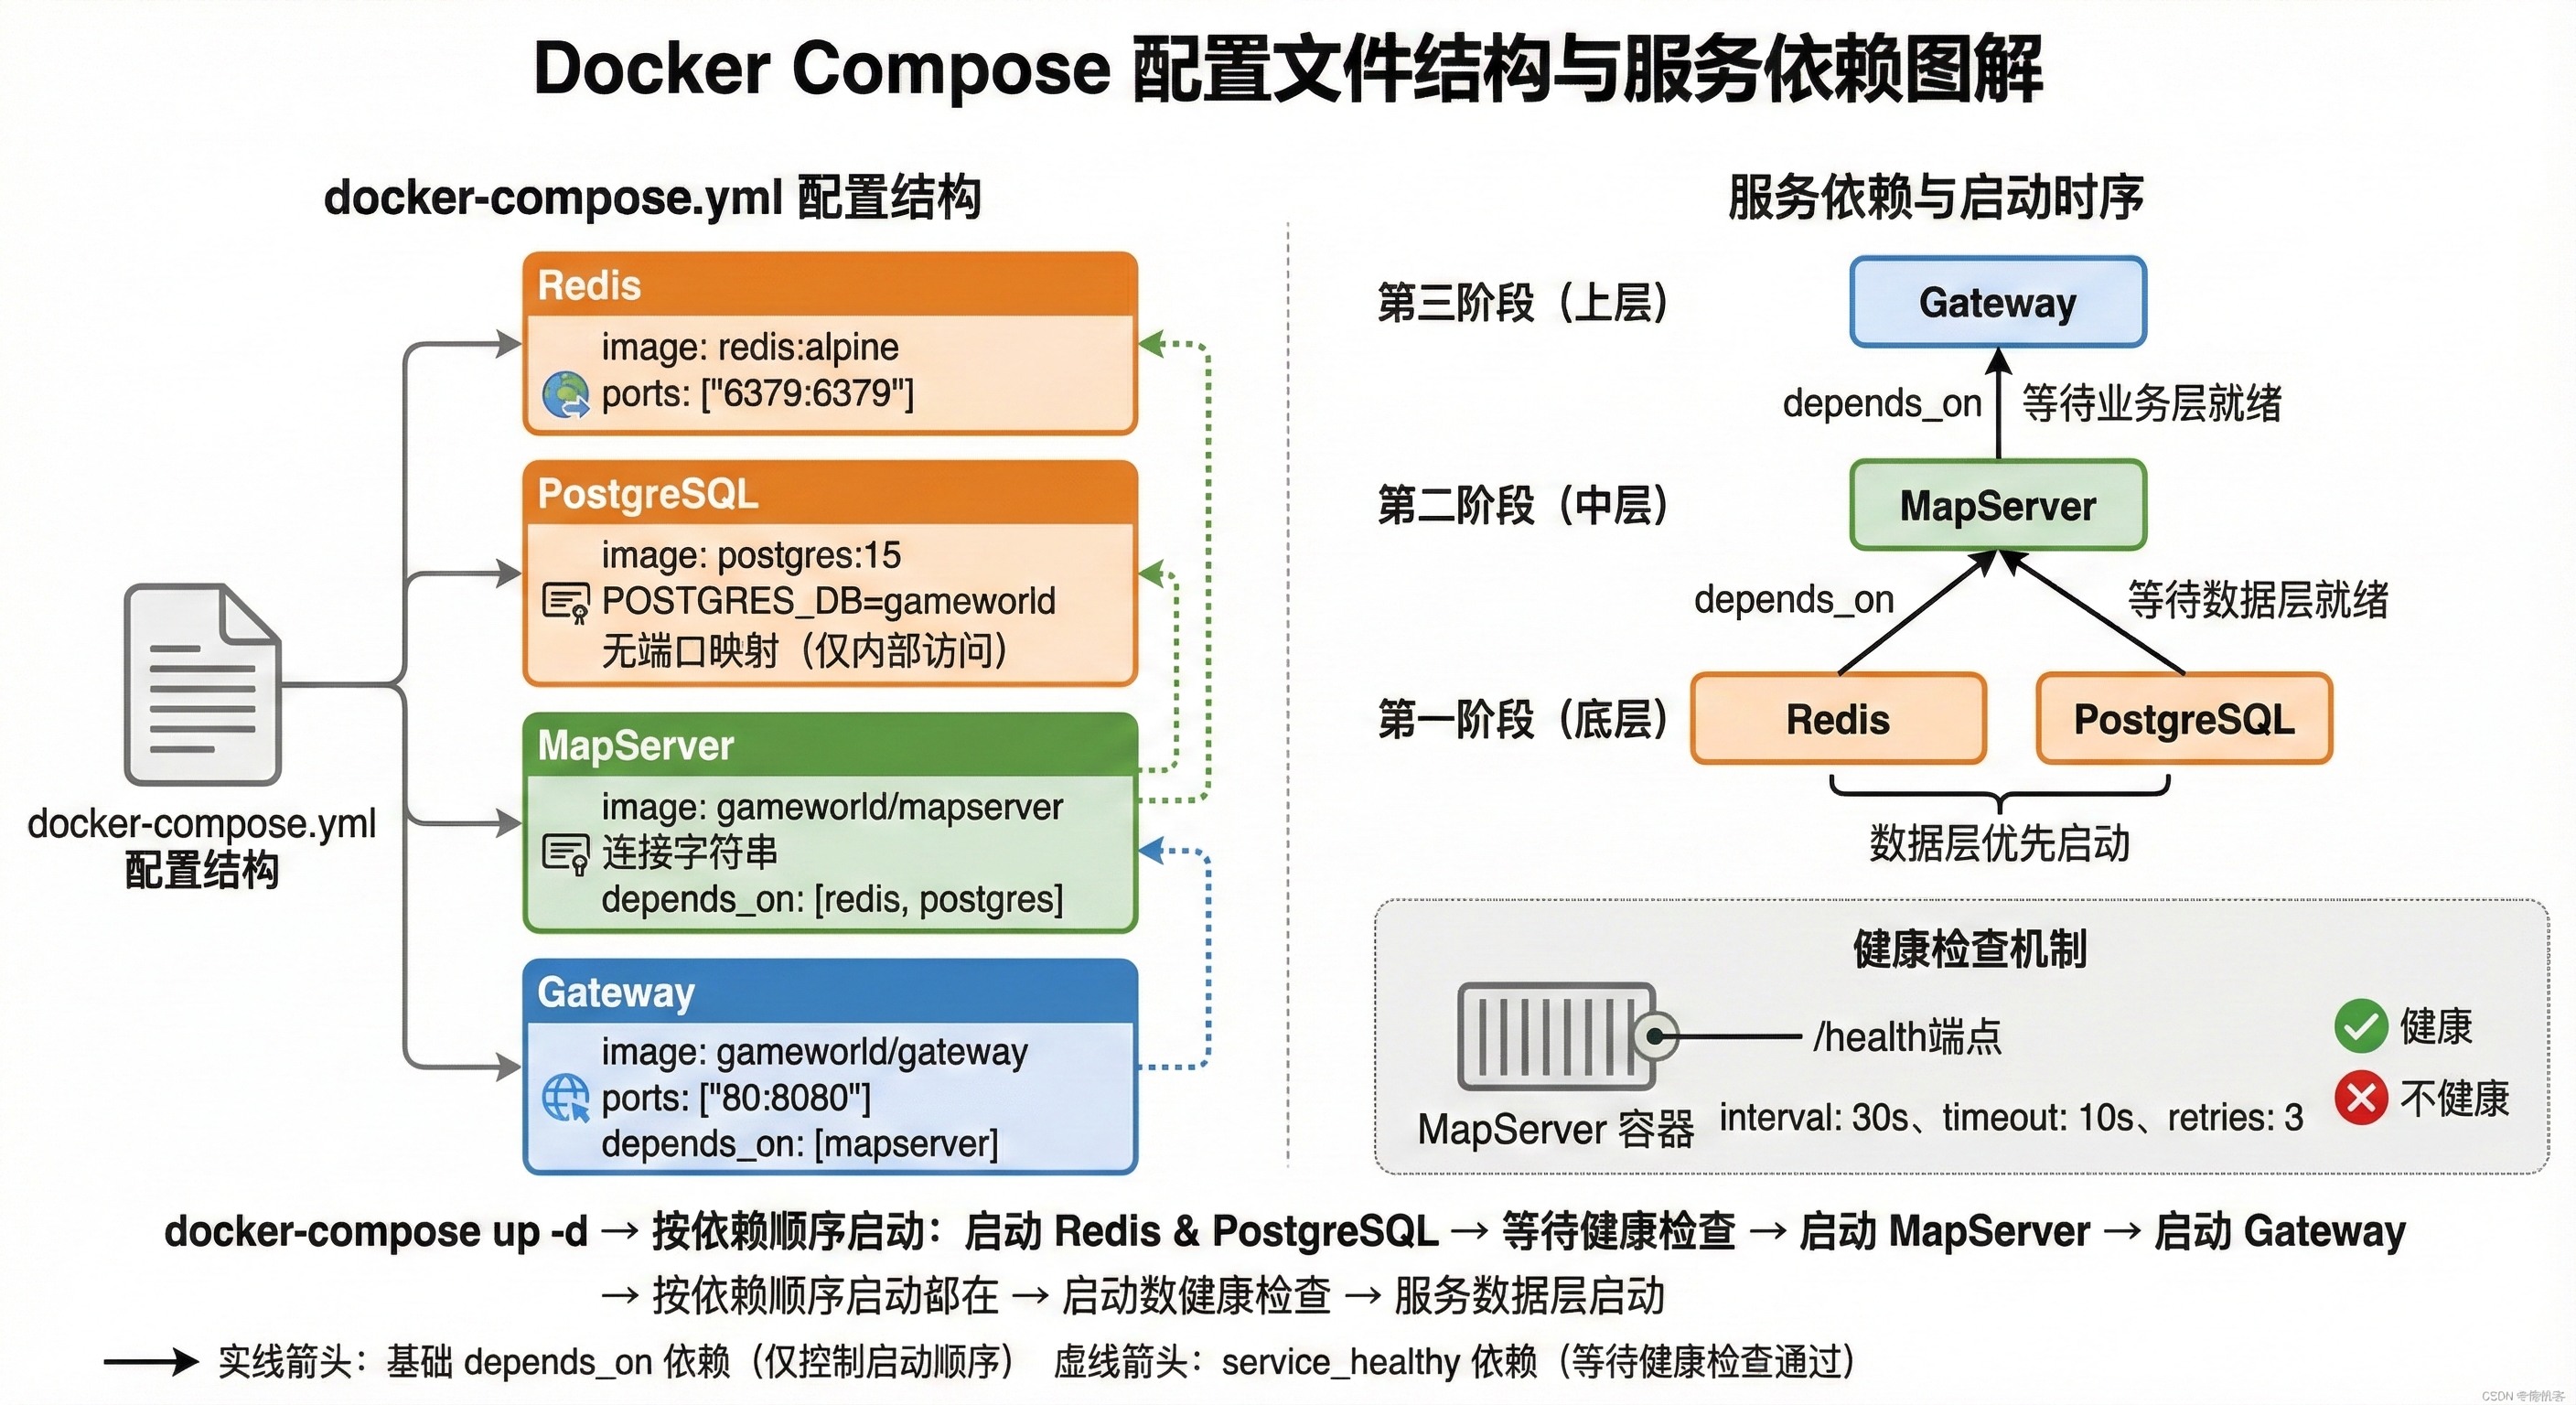
\includegraphics[width=0.85\textwidth]{figures/sec5/Docker_Compose_config.png}
\caption{Docker Compose 配置文件结构与服务依赖图解}
\label{fig:compose-config}
\end{figure}

\subsubsection{网络通信:构建服务间的``高速公路''}

在传统的单机应用中,不同模块之间通过函数调用进行通信;而在容器化的微服务架构中,服务间的通信需要通过网络来实现。Compose 为同一配置文件中的所有服务自动创建了一个内部网络,这个网络就像是为微服务架构专门修建的``高速公路系统''。

如图 \ref{fig:compose-concepts} 右下角的网络通信与安全策略图所示,在这个内部网络中,每个服务都有一个基于服务名的``网络身份证''。地图服务想要连接 Redis(端口 6379),不需要知道 Redis 容器的具体 IP 地址,只需要使用服务名``redis''就能建立连接。这种``服务发现''机制极大地简化了微服务间的通信配置,也提供了良好的扩展性基础——当我们需要将单个 Redis 服务扩展为 Redis 集群时,服务名会自动负载均衡到所有实例,上游服务无需做任何修改。

更重要的是,这个内部网络是与外部世界隔离的,只有明确配置了端口映射的服务才能从外部访问。如图中所示,网关服务映射端口 80:8080 供外部访问,而数据库服务则只接受内部访问,提供了天然的安全隔离——数据库服务只需要响应来自业务层的内部请求,而无需担心来自外部的恶意访问。

网络通信的分层特征也与我们的架构设计完美契合。数据层的服务主要接受来自业务层的连接请求;业务层的服务既要向下连接数据服务,又要向上响应接入层的调用;接入层的服务则需要同时处理外部用户请求和内部服务调用。这种清晰的通信模式不仅提升了系统的可理解性,也为性能优化和安全控制提供了明确的边界。

\subsubsection{端口策略:在可访问性与安全性之间找到平衡}

端口映射是连接容器内部服务与外部世界的桥梁,但在生产环境中,我们不能简单地将所有端口都暴露给外部。合理的端口映射策略需要在服务的可访问性与系统的安全性之间找到最佳平衡点。

对于面向用户的服务,如网关服务,应该映射到标准的 HTTP/HTTPS 端口(80/443),这样用户就能通过标准的域名访问游戏服务,无需记忆复杂的端口号。这类服务的端口映射策略应该优先考虑用户体验和访问便利性。如图 \ref{fig:compose-config} 所示,Gateway 服务通过配置 \texttt{ports: ["80:8080"]} 实现对外服务发现。

对于运维管理性质的服务,如监控面板、管理控制台等,可以映射到非标准端口(如 8080、9090),这样既能提供必要的访问能力,又能避免与其他应用发生端口冲突。同时,这类端口通常只开放给内部网络或特定的管理人员,增加了一层安全保障。

而对于数据库、缓存等基础设施服务,则需要谨慎考虑是否对外暴露。如图 \ref{fig:compose-config} 中 PostgreSQL 服务的配置所示,数据库通过 \texttt{POSTGRES\_DB=gameworld} 等环境变量进行配置,但没有端口映射,采用``无端口映射(仅内部访问)''策略。在开发和测试环境中,为了便于调试和数据查看,可能需要临时暴露这些服务的端口;但在生产环境中,这些服务应该只在容器内部网络中可见,通过业务层服务来间接访问,这样能最大化地降低安全风险。

图 \ref{fig:compose-config} 清晰地展示了整个服务依赖与启动时序的全貌。从左侧的配置文件结构,到右侧的服务依赖关系图,我们可以看到:第一阶段数据层优先启动,第二阶段 MapServer 等待数据层就绪后启动,第三阶段 Gateway 等待业务层就绪后启动。底部的启动流程说明了完整的编排过程:执行 \texttt{docker-compose up -d} 命令后,系统按依赖顺序启动服务,等待健康检查通过,最终完成整个服务栈的部署。

这种分层的端口映射策略体现了``最小权限原则''——只暴露必要的服务端口,将安全风险降到最低。同时,这种策略也提供了良好的灵活性,我们可以根据不同环境的需求来调整端口映射配置,而不影响服务间的内部通信逻辑。

至此,我们已经理解了 Docker Compose 编排多服务应用的核心概念和设计原则。通过服务分层、依赖控制和网络策略的有机结合,原本需要手工协调的复杂启动流程被抽象为清晰的配置声明。这种标准化的编排方式不仅大大降低了部署的复杂度和出错概率,更重要的是为团队协作和系统演进提供了坚实基础。在下一节中,我们将把视野从单机编排扩展到集群管理,探索如何让游戏服务真正具备工业级的高可用和弹性扩展能力。


%\subsection{踏上云端：从本地上云}
%\paragraph{本节目标} 理解上云本质，掌握 “选服务器 - 传镜像 - 启动服务” 流程。
%\paragraph{写作建议} 
%\begin{enumerate}
%    \item 列上云优势：性能弹性、公网访问、宕机重启。
%    \item  分 3 步：选带 Docker 的云服务器、传镜像（仓库下载 / 直接拷贝）、启动服务 + 开安全组端口。
%\end{enumerate}

\subsection{踏上云端：从本地上云} % 加到附录里 

\subsubsection{云端优势：为什么要离开舒适圈}

当我们在本地机器上成功搭建起完整的游戏服务栈后，很容易产生一种"万事俱备"的错觉。然而，真正的挑战往往隐藏在看似平静的表面之下。本地环境有着三个致命的局限性，阻碍着我们的游戏世界向更广阔的玩家群体开放。

首先是网络可达性的天然屏障。家用网络环境通常位于 NAT（网络地址转换）之后，外部玩家根本无法直接连接到你电脑上运行的游戏服务。即便通过端口转发等技术手段勉强打通连接，家用宽带的上行带宽也极其有限，往往只有几 Mbps，难以支撑多人同时在线的实时交互需求。这意味着无论你的代码多么优雅，架构多么精妙，玩家都无法真正体验到你精心构建的游戏世界。

其次是可靠性的根本缺陷。个人电脑并非为 7×24 小时不间断运行而设计，停电、死机、网络中断都是家常便饭。更要命的是，当你需要重启电脑、安装软件或者简单的合上笔记本时，整个游戏世界就会瞬间消失，所有在线玩家的体验都会被粗暴地中断。这种不可控的中断对于强调连续性和沉浸感的在线游戏来说，是绝对无法接受的用户体验。

最后是扩展能力的根本约束。单台个人电脑的计算资源是固定的，当游戏火爆、玩家激增时，你无法像变魔术一样突然增加内存或 CPU 核心数。相反，云端基础设施提供了近乎无限的资源弹性：需要更多计算力时可以一键扩容，流量下降时可以自动缩容节约成本。这种动态调节能力是应对互联网业务波动性的关键武器。

云端部署的价值正是要彻底解决这三大痛点：通过公有云厂商的高质量网络基础设施获得优秀的网络连通性和带宽保障；借助专业级的硬件设备和电力保障实现真正的高可用运行；利用弹性计算资源实现按需扩缩容，让系统具备应对流量洪峰的能力。这不仅是技术架构的升级，更是产品从“概念验证”向“商业可行”的关键跃迁。

\begin{figure}[htbp]
\centering
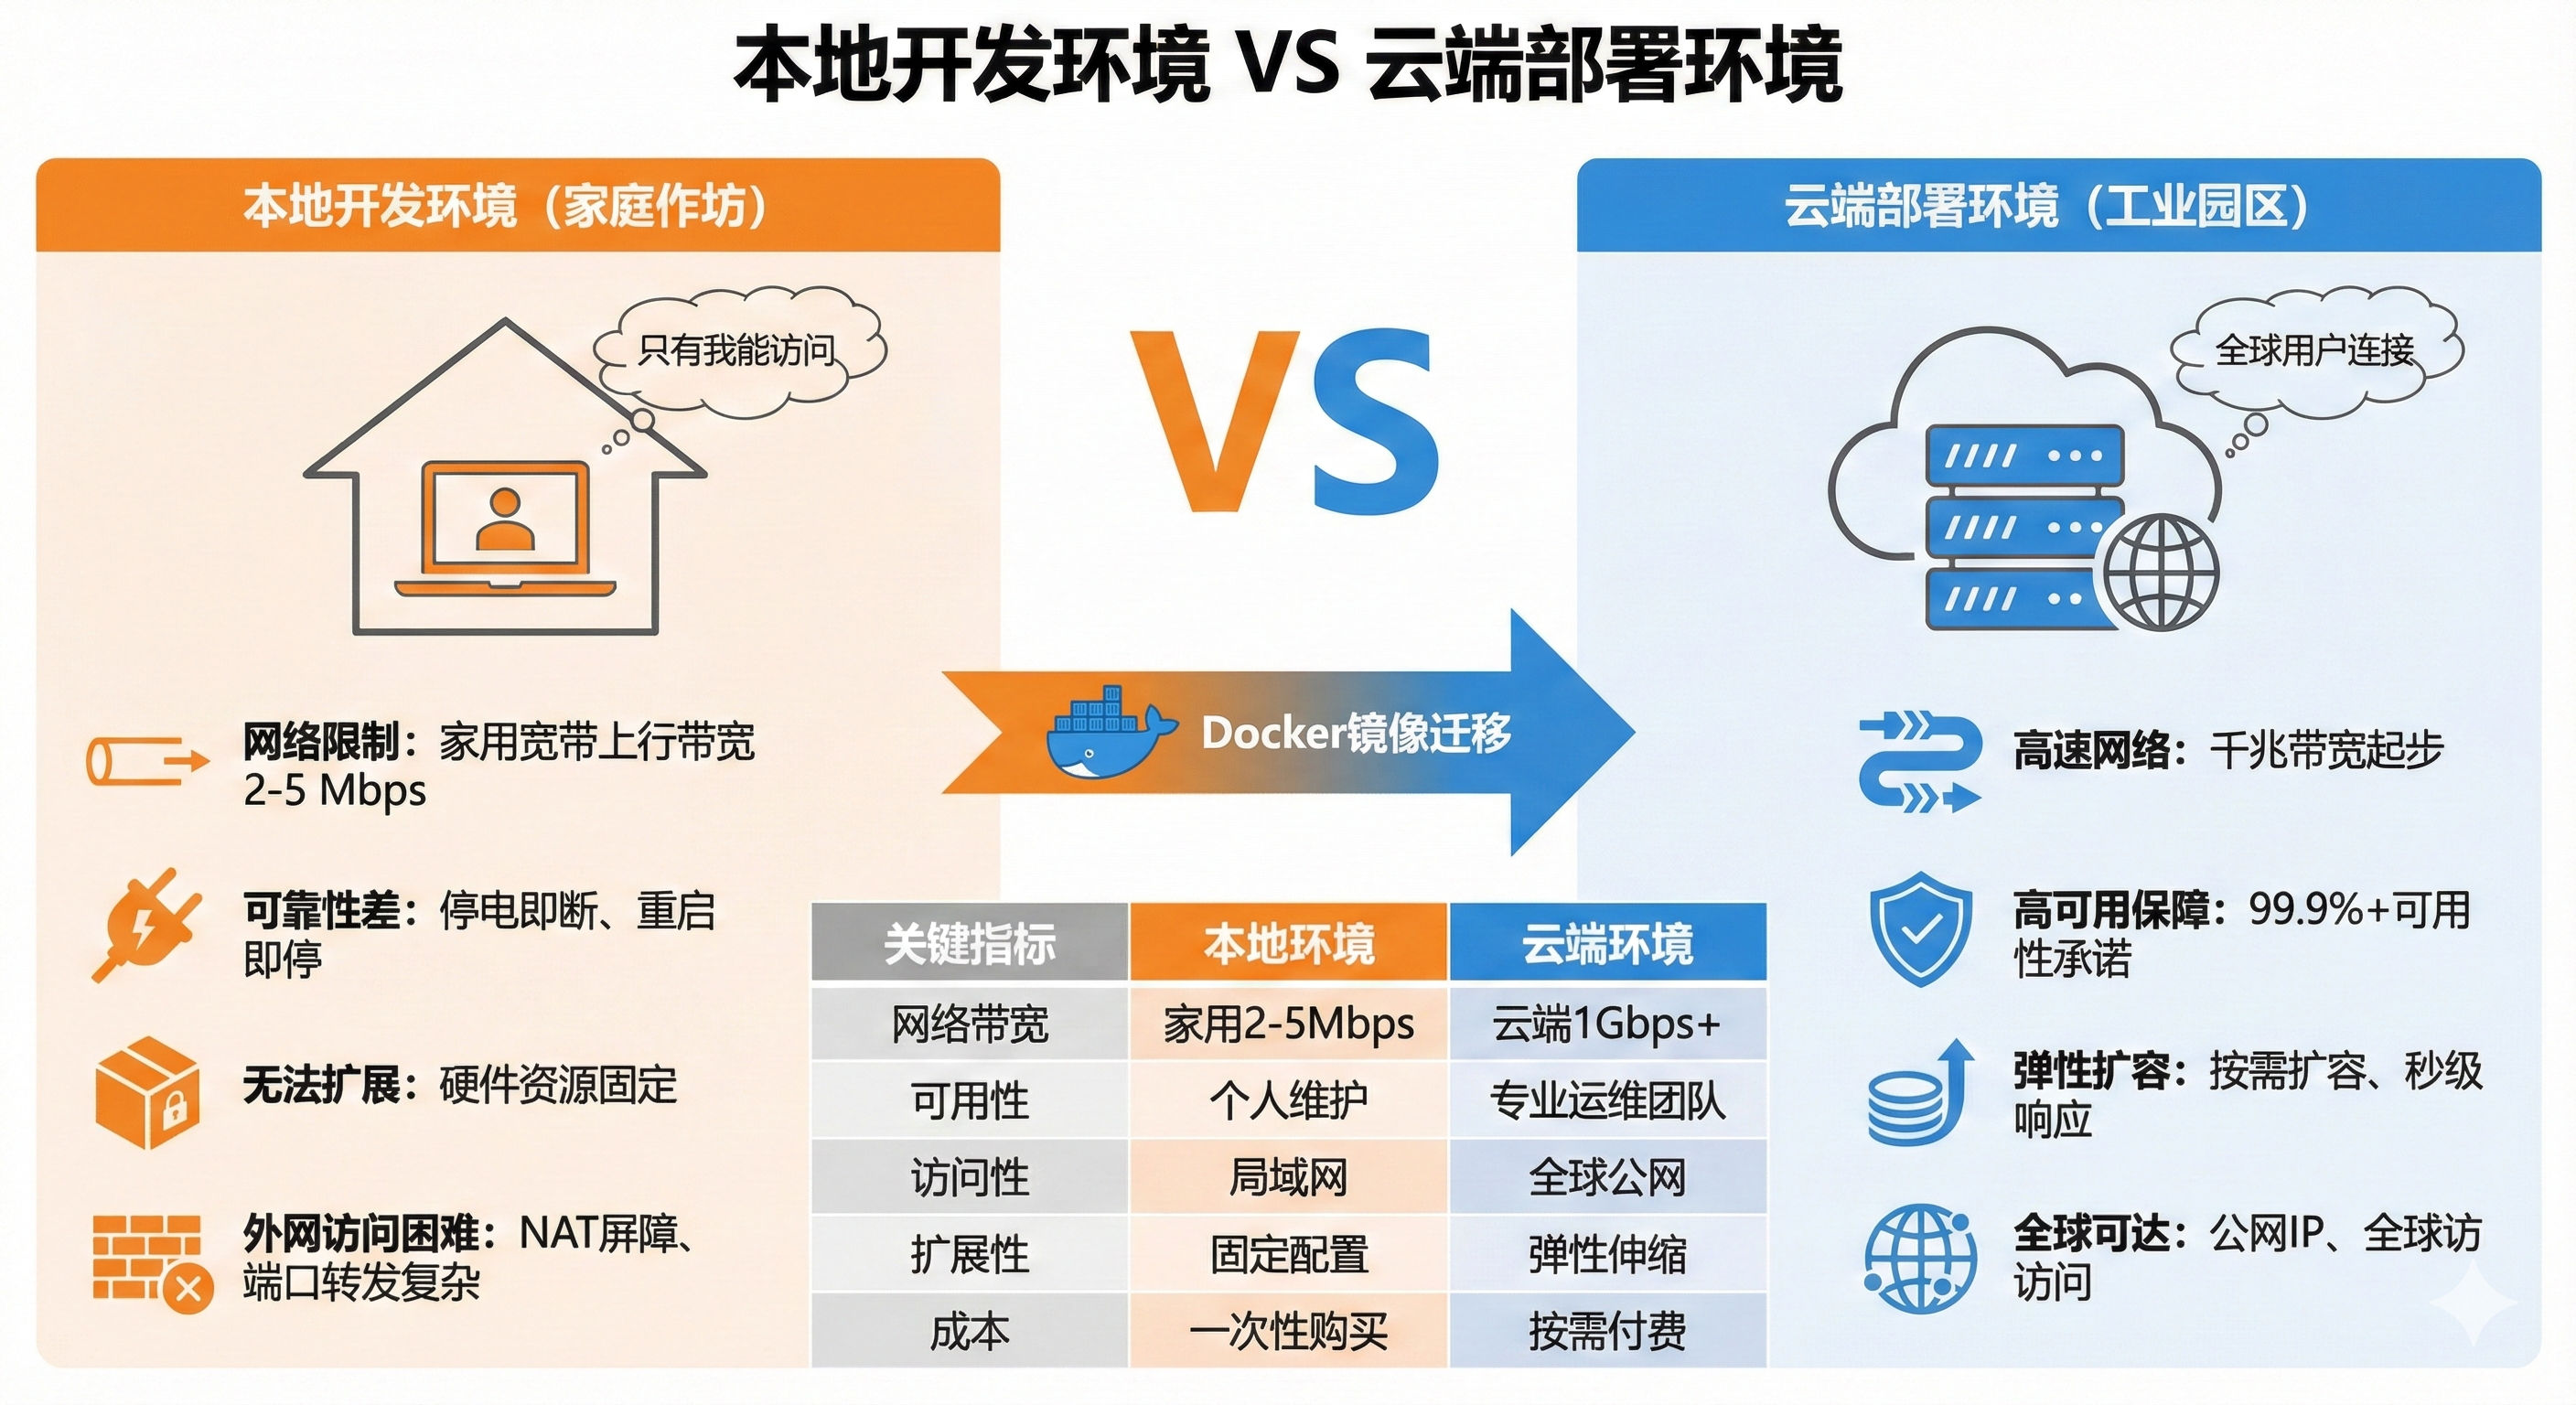
\includegraphics[width=0.9\textwidth]{figures/sec5/local-vs-cloud-environment.png}
\caption{本地开发环境与云端部署环境的全面对比}
\label{fig:local-vs-cloud}
\end{figure}

如图\ref{fig:local-vs-cloud}所示，从家庭作坊式的本地开发环境向工业级的云端部署环境迁移，不仅仅是硬件配置的提升，更是从个人实验向商业服务的根本转变。

\subsubsection{选择云端战场：配置你的虚拟战舰}

在决定将游戏世界搬到云端之后，我们面临的第一个实际问题就是：到底该选择什么样的云服务器？这个决策看似复杂，实际上可以用一个简单的对比来理解——就像从家里的小作坊升级到工业园区的标准厂房。

我们之前在本地开发时使用的个人电脑，就像是自己家里的一间小作坊：电源稳定性一般（停电就断），网络带宽有限（家用宽带上行只有几Mbps），而且只有你自己能进入（局域网访问）。更要命的是，一旦你的电脑关机或重启，整个“作坊”就停止运营了，所有的“客户”都会被拒之门外。

而云服务器则完全不同，它更像是工业园区里的标准化厂房：有不间断电源保障，配备高速光纤网络，24小时专业维护团队，全世界的客户都能轻松找到你的地址。最关键的是，如果业务扩张需要更大空间，你可以随时申请相邻的厂房进行扩容，而不用重新选址搬迁。

对于我们这种刚刚起步的游戏项目，配置选择其实并不复杂。大部分云厂商都提供了针对不同应用场景的推荐配置，我们只需要按照官方的入门指南来选择即可。通常来说，支持几十到几百名在线玩家的游戏服务，选择2-4核CPU、4-8GB内存的基础配置就足够了。操作系统建议选择Ubuntu 20.04 LTS，因为它对Docker的支持最为成熟，相关的教程和社区资源也最丰富。

更重要的是选择合适的地理位置。如果你的玩家主要在国内，选择华东或华北地区的数据中心能够提供最佳的网络延迟；如果面向海外玩家，则需要选择离目标用户更近的海外节点。这就像开实体店一样，位置的选择直接影响客流量和用户体验。

云服务器的真正价值不在于配置有多强大，而在于它提供的可靠性和可达性保障。当我们的游戏世界部署在云端后，它就变成了一个真正的“永不下线”的在线世界，全球的玩家都能随时随地进入并享受稳定的游戏体验。

\subsubsection{理解上云本质：从孤岛到互联网}

上云的核心不是简单的“换个地方放服务器”，而是一次架构思维的根本转变。在本地开发阶段，我们构建的是一个“孤岛式”的封闭系统：所有组件都在同一台机器上，通过本地网络通信，只有开发者能够访问。而上云意味着将这个封闭系统转变为开放的互联网服务，需要考虑的问题维度完全不同。

从技术架构角度看，上云过程实际上是在解决三个层次的连接问题。第一层是物理连接：确保云服务器具备稳定的网络接入能力，这包括带宽保障、延迟优化以及网络冗余等基础设施问题。第二层是逻辑连接：通过合理的端口映射和防火墙配置，让外部客户端能够正确找到并连接到我们的游戏服务。第三层是业务连接：确保服务在面对真实用户流量时能够稳定运行，这涉及并发处理、错误恢复、性能监控等运维层面的考虑。

更深层次地看，上云还意味着运维模式的转变。本地开发时，我们更多关注的是功能实现和逻辑正确性；而在云端环境中，服务的可观测性、可恢复性、可扩展性变得同样重要。这就需要我们在设计和部署服务时，从一开始就考虑日志收集、健康检查、优雅关闭等生产级特性。

\begin{figure}[htbp]
\centering
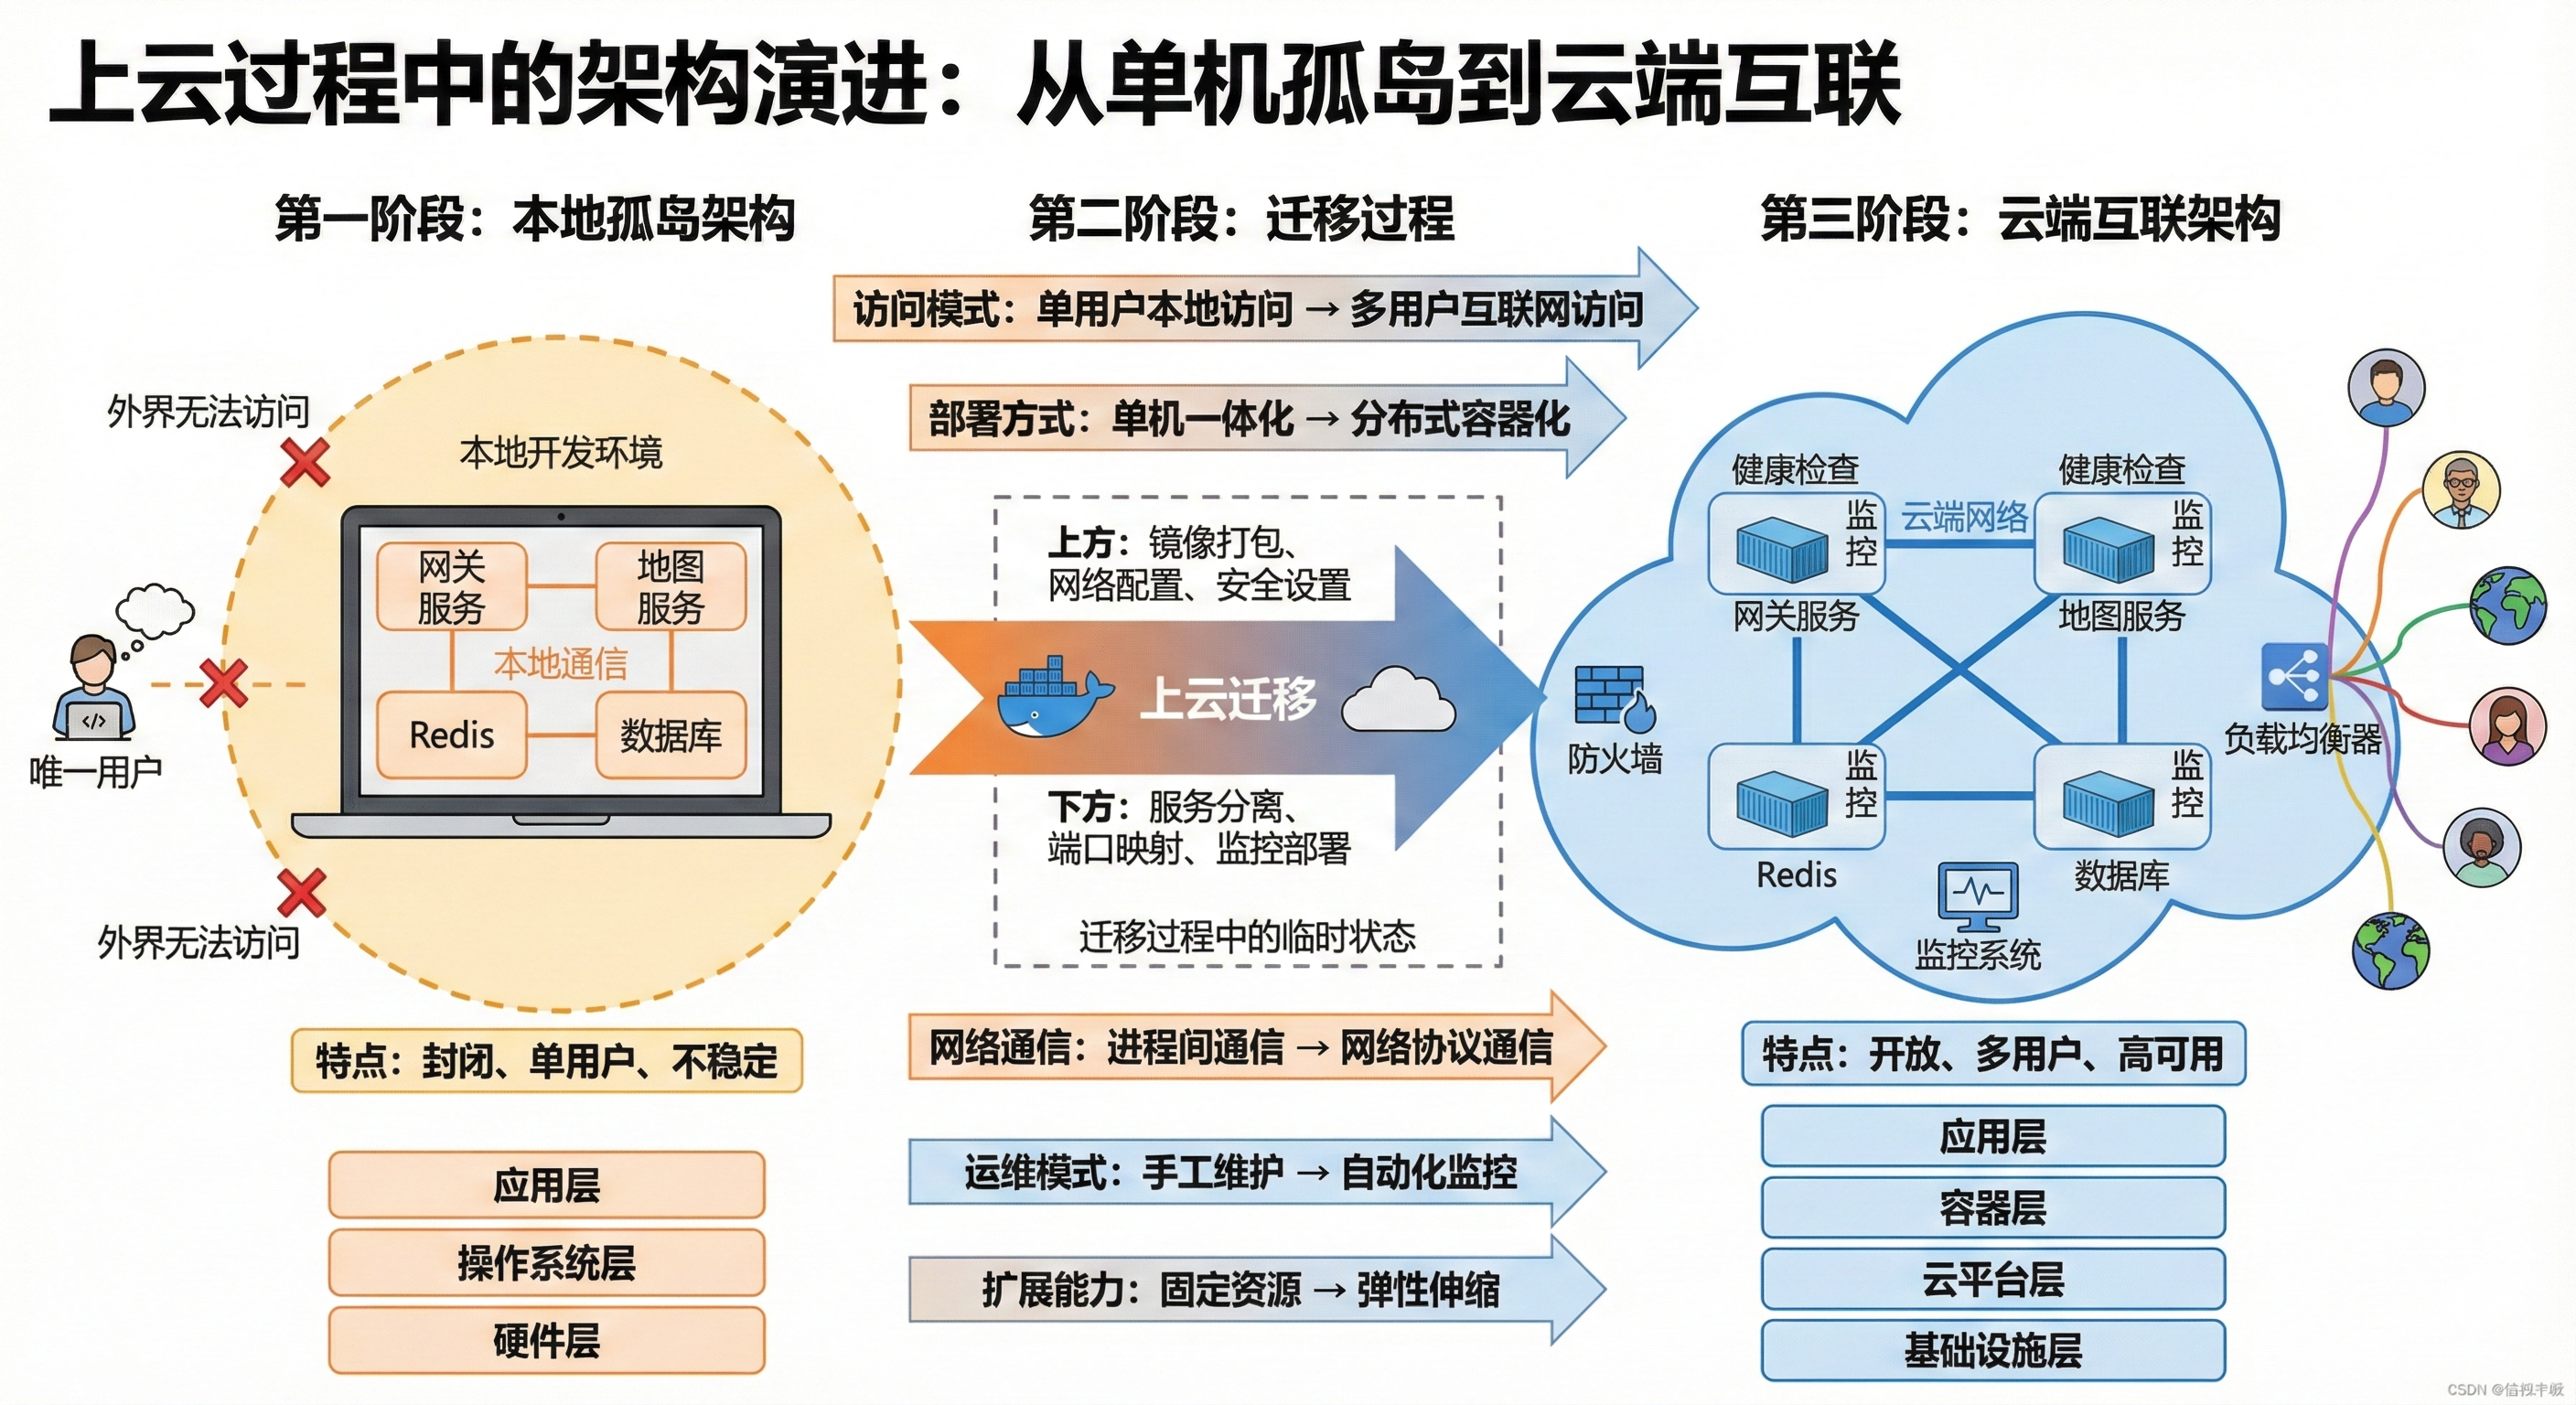
\includegraphics[width=0.9\textwidth]{figures/sec5/cloud-migration-architecture.png}
\caption{上云过程中的架构演进：从单机孤岛到云端互联}
\label{fig:cloud-migration}
\end{figure}

如图\ref{fig:cloud-migration}所示，上云不是简单的平移，而是整个系统架构从封闭走向开放、从静态走向动态的演进过程。

\subsubsection{镜像迁移：代码的跨环境旅行}

将我们在本地构建的Docker镜像传输到云端环境，是上云流程中最关键的技术环节。这个过程的本质是让我们的应用代码完成一次“跨环境旅行”，从开发者的本地机器迁移到云端的生产环境。

这个迁移过程面临着几个核心挑战。首先是传输效率问题：Docker镜像通常体积较大，从几百MB到几个GB不等，如何在有限的网络带宽下快速可靠地完成传输，直接影响部署效率。其次是版本一致性问题：如何确保云端运行的镜像与本地构建的镜像完全一致，避免因为环境差异导致的运行时问题。最后是安全性问题：在镜像传输和存储过程中，如何保护应用代码和敏感配置不被泄露。

最推荐的做法是利用镜像仓库机制来实现镜像的分发。这个过程类似于我们使用应用商店下载手机APP：开发者先将应用上传到商店（推送镜像到仓库），用户再从商店下载到自己设备（从仓库拉取镜像到云服务器）。

镜像仓库的核心优势在于其分层存储机制。Docker镜像本质上是由多个层（Layer）叠加而成的，当我们推送镜像时，仓库会智能地识别哪些层是新的、哪些层是重复的。这意味着后续的版本更新只需要传输变化的部分，大大提升了传输效率。

在选择镜像仓库时，我们有多种选择。Docker Hub是最常用的公共仓库，免费用户可以创建无限数量的公开镜像，但私有镜像数量有限制。各大云厂商也提供了自己的容器镜像服务，如阿里云的容器镜像服务ACR、腾讯云的容器镜像服务TCR等，这些服务通常提供更好的国内访问速度和更丰富的企业级功能。

\begin{figure}[htbp]
\centering
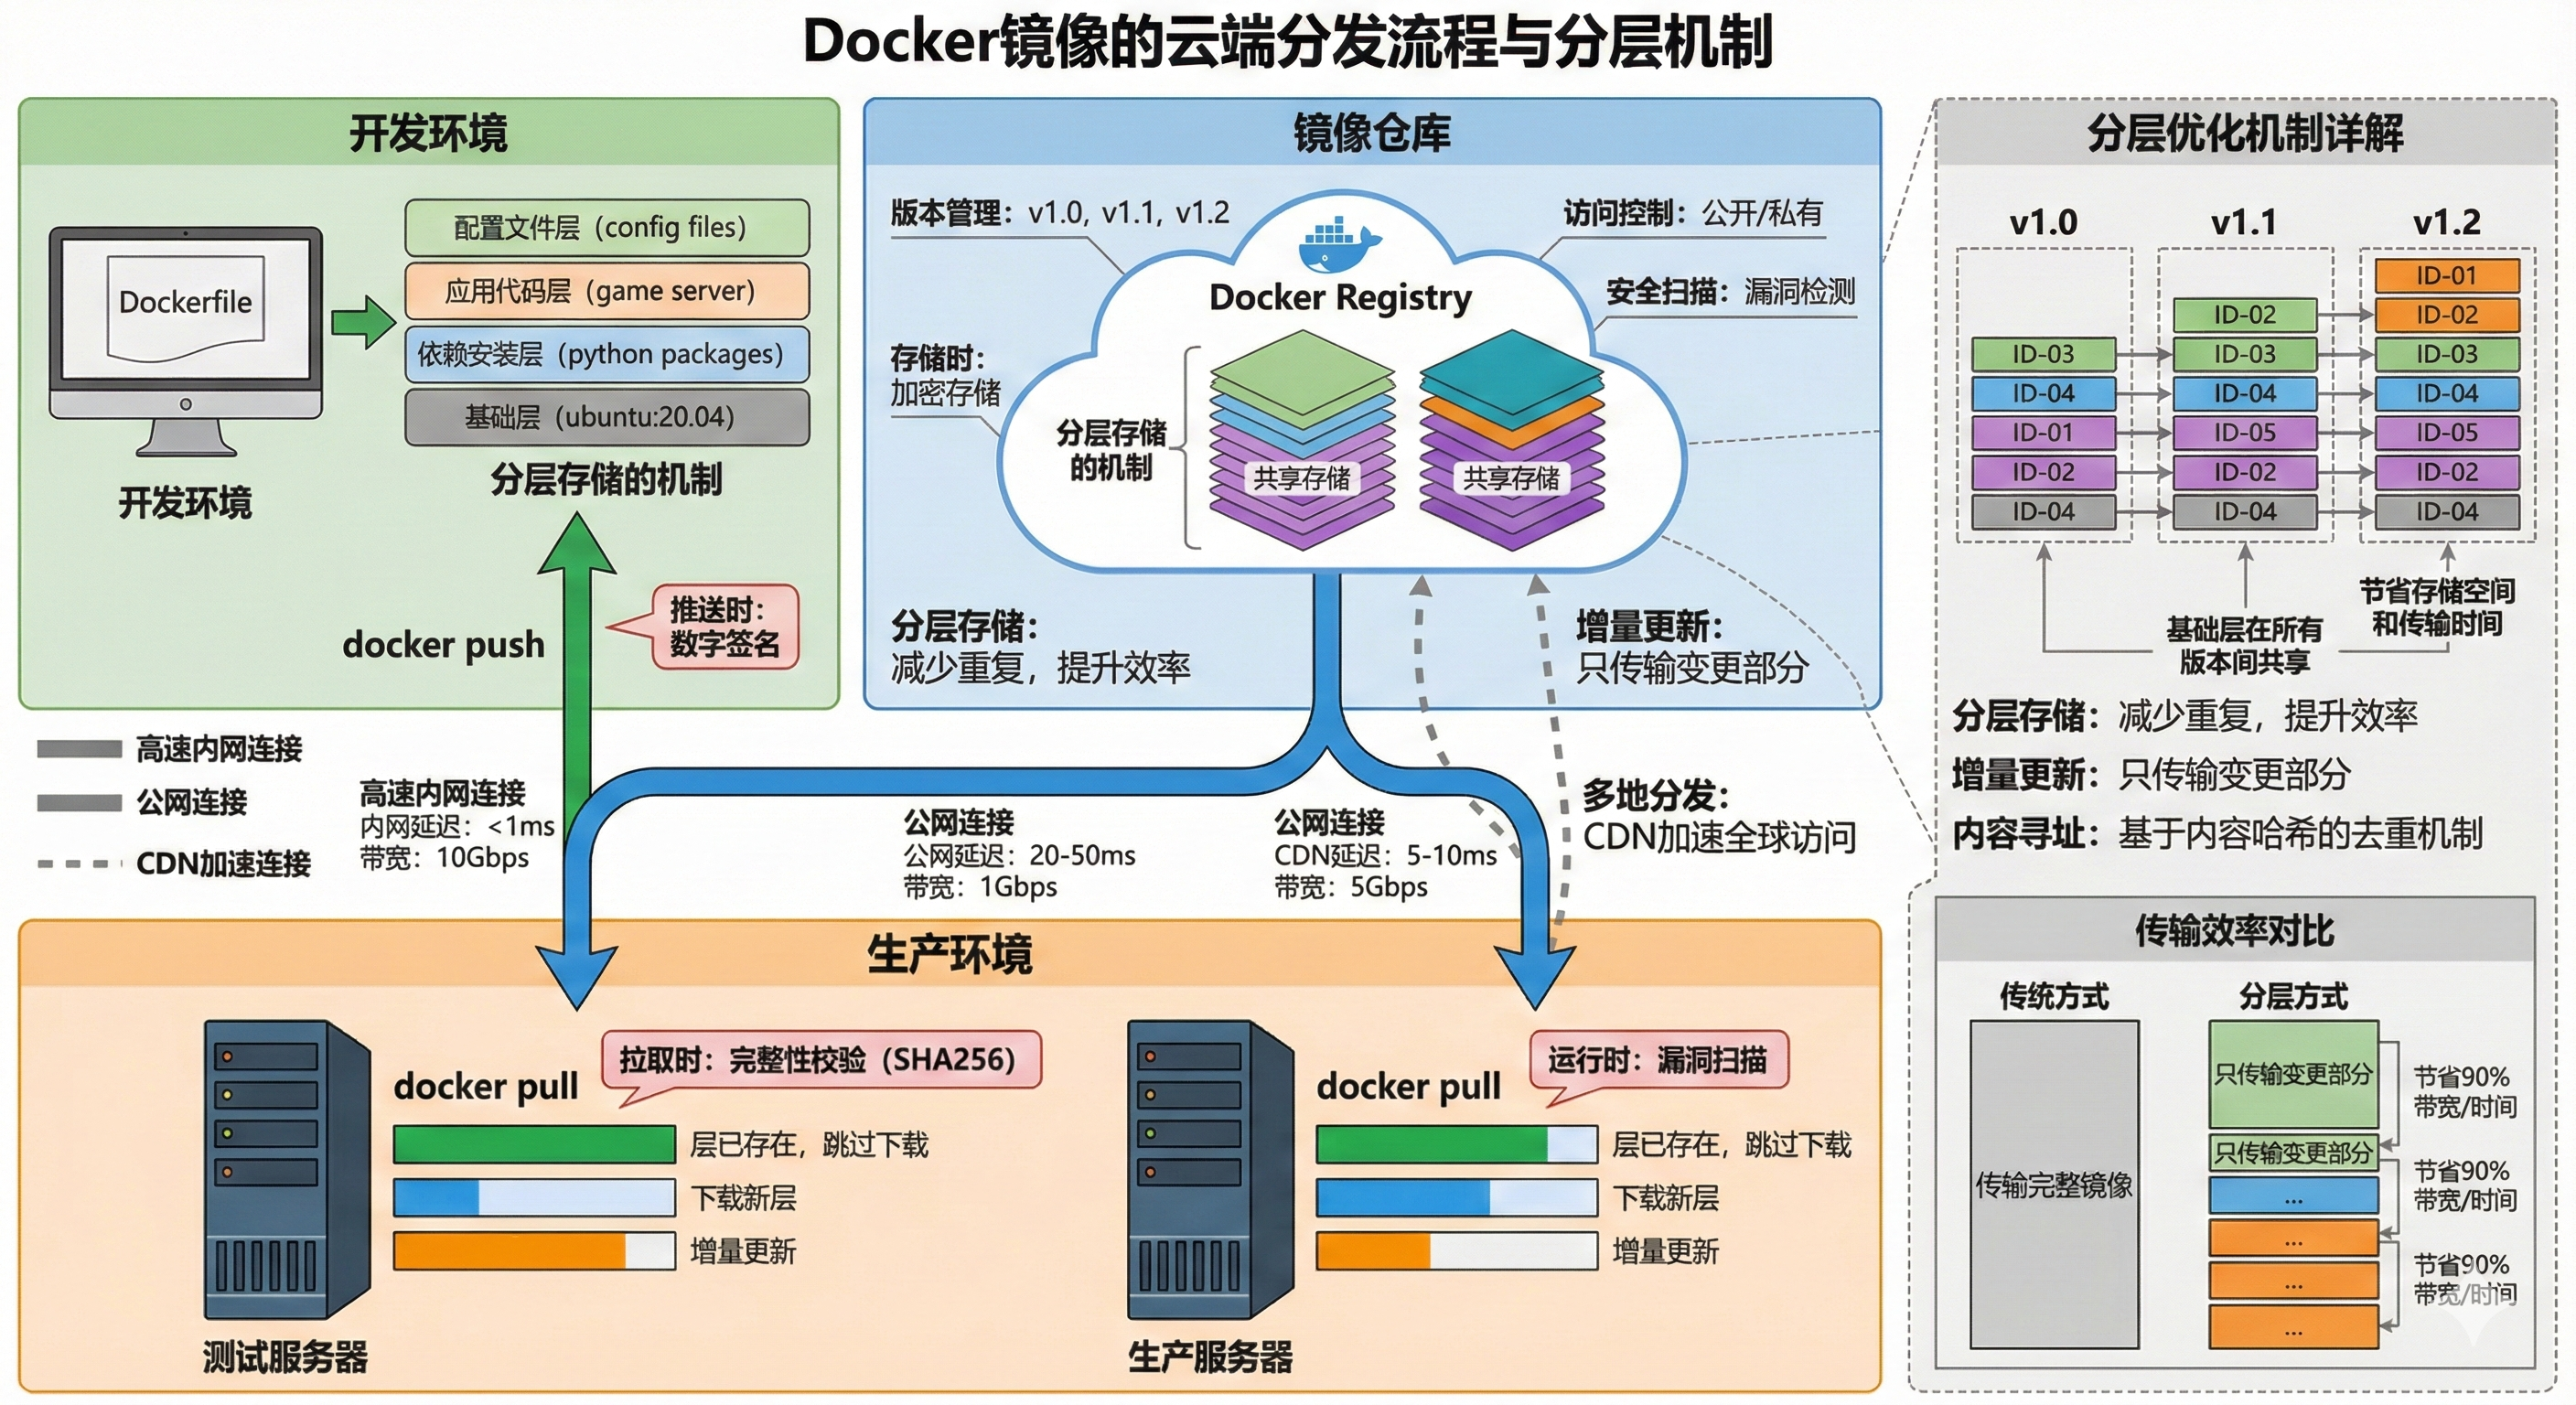
\includegraphics[width=0.9\textwidth]{figures/sec5/docker-image-distribution.png}
\caption{Docker镜像的云端分发流程与分层机制}
\label{fig:image-distribution}
\end{figure}

对于对安全性要求较高或网络环境特殊的场景，也可以选择直接文件传输的方式。这种方法将镜像导出为文件，然后通过文件传输工具将其上传到云服务器，最后重新导入镜像。虽然这种方式缺乏仓库机制的便利性，但在某些企业内网环境或对数据流向有严格管控的场景下，这种点对点传输方式反而更加合适。

无论采用哪种传输方式，都强烈建议在传输完成后进行完整性校验。通过比较本地和远程镜像的摘要值，可以确保传输过程中没有发生数据损坏。这种看似多余的验证步骤，往往能在关键时刻避免因为镜像损坏导致的莫名其妙的运行时错误。

\subsubsection{网络配置：为服务打开通往世界的大门}

成功将镜像传输到云端并启动服务后，最后一个关键步骤就是配置网络访问策略。如果说镜像迁移是让应用“安家落户”，那么网络配置就是为这个新家“开门接客”的过程。

云环境的网络安全机制相比本地环境要严格得多，遵循的是“默认拒绝，显式允许”的安全原则。这意味着新启动的云服务器几乎所有端口都是关闭的，我们需要根据业务需求，显式地为每个需要对外提供服务的端口开放访问权限。

云厂商通常通过“安全组”（Security Group）机制来管理网络访问规则。安全组本质上是一套网络防火墙规则的集合，可以精确控制哪些来源IP、哪些端口、哪些协议被允许访问你的服务器。

安全组的工作原理类似于小区的门禁系统。你需要为每类访客（不同类型的网络请求）制定不同的准入规则：普通访客（游戏玩家）可以通过大门（游戏端口）进入；快递员（监控系统）可以通过特定入口（监控端口）送货；而维修人员（运维管理）则需要特殊权限（SSH端口）才能进入核心区域。

对于我们的游戏服务，通常需要配置以下几类规则：HTTP/HTTPS端口用于网页版游戏或API接口访问，WebSocket端口用于实时通信，以及可能的自定义端口用于游戏专有协议。这些服务端口通常需要向全球开放，以便世界各地的玩家都能访问。同时，SSH管理端口应该严格限制访问来源，只允许运维人员的固定IP地址访问。如果架构中包含多台服务器之间的内部通信，这些端口只需要对内网其他服务器开放。

\begin{figure}[htbp]
\centering
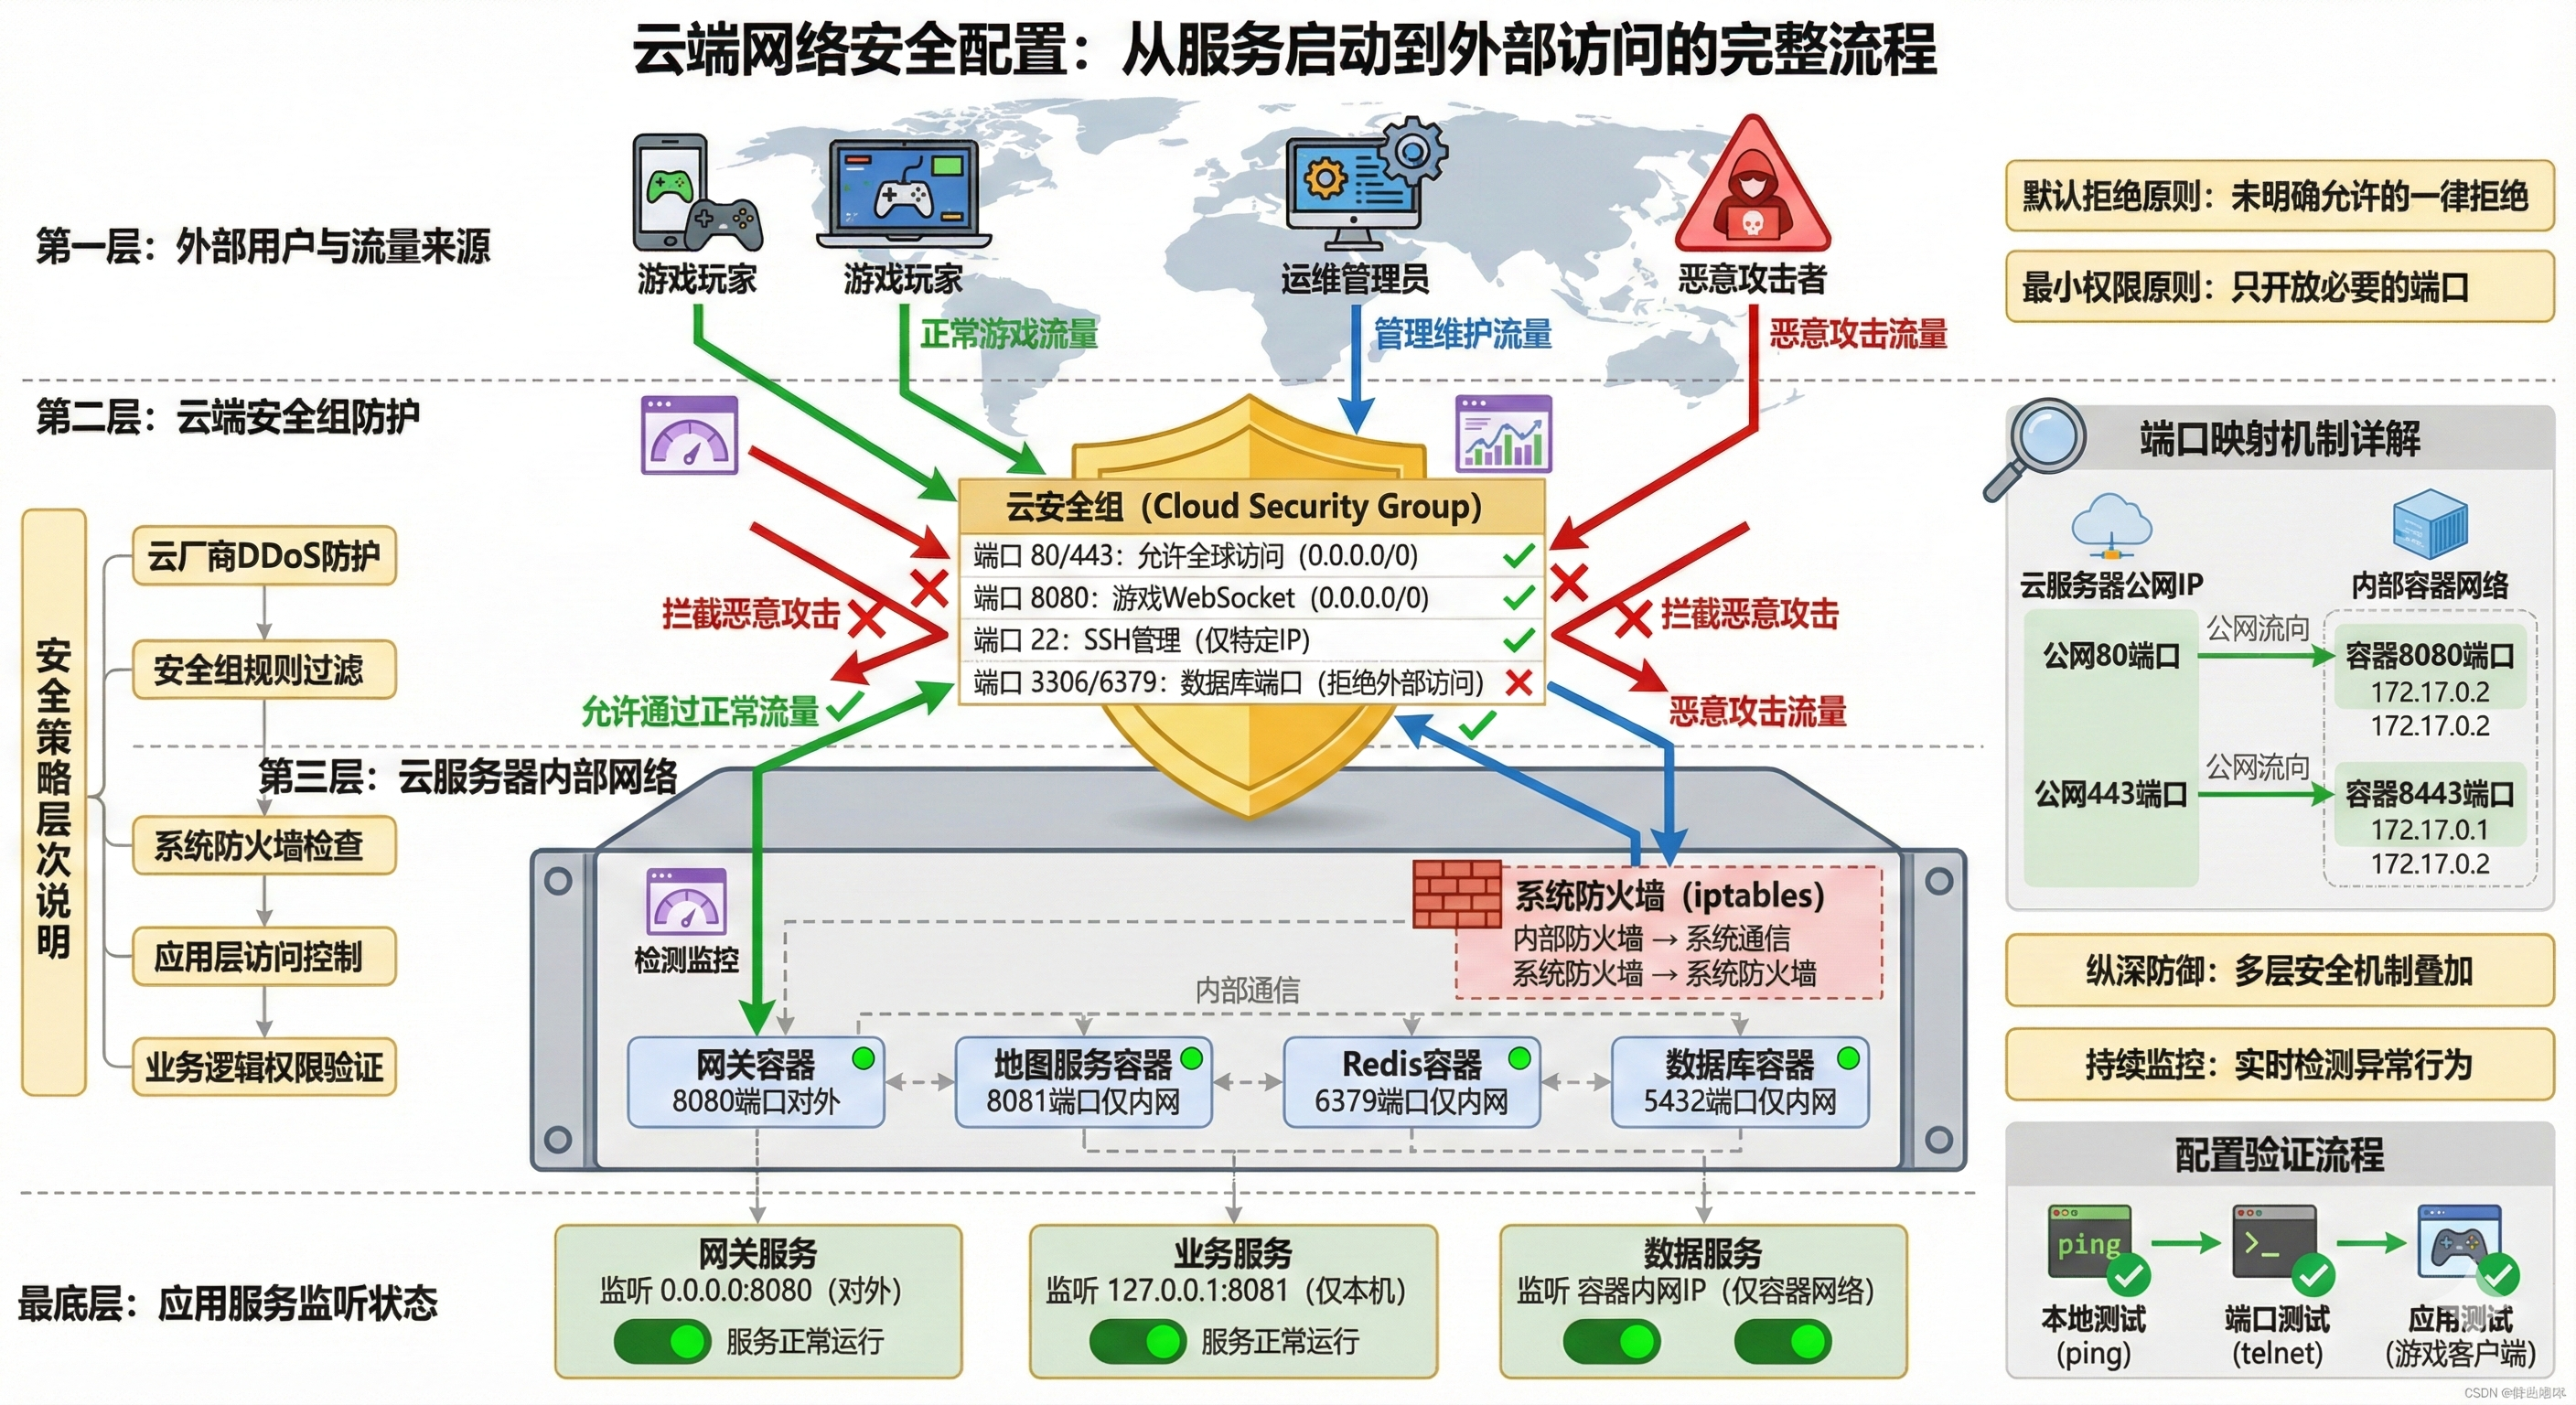
\includegraphics[width=0.9\textwidth]{figures/sec5/cloud-network-security.png}
\caption{云端网络安全配置：从服务启动到外部访问的完整流程}
\label{fig:network-security}
\end{figure}

配置完安全组规则后，强烈建议进行端到端的连通性测试。这个过程就像检查水管是否通畅一样，我们需要确保数据包能够顺利地从外部客户端传输到我们的游戏服务。

测试方法可以从简单到复杂逐步进行。最基础的测试是检查服务器是否可达；进一步可以测试特定端口是否开放；最完整的测试是从实际的游戏客户端发起连接，验证整个应用层协议是否正常工作。

在测试过程中，如果发现连接问题，需要逐层排查：首先检查云服务器的安全组配置是否正确；然后检查服务器内部的防火墙设置；最后确认游戏服务本身是否正常运行并监听在正确的端口上。

通过云端监控工具观察服务器的网络流量、连接数、响应时间等关键指标，也能帮助我们及时发现和解决网络问题。当看到监控面板上出现来自全球各地的连接请求时，就意味着我们的游戏世界真正向全世界开放了。

\subsubsection{从概念到现实：完成上云的最后一跃}

通过以上四个步骤——认识上云价值、选择云端资源、迁移应用镜像、配置网络访问——我们成功地将游戏服务从本地环境迁移到了云端。这不仅仅是一次简单的环境迁移，更是从个人项目向互联网服务的根本转变。

这种转变带来的影响是深远的。从技术角度看，我们获得了更强的可靠性、更好的性能表现、以及面向未来的扩展能力；从产品角度看，游戏从一个只有开发者能体验的原型，变成了全球玩家都能访问的实际服务；从团队角度看，这为后续的协作开发、持续集成、运维监控等工程化实践奠定了基础。

然而，上云只是万里长征的第一步。真正的工业级应用还需要考虑高可用架构、自动化运维、弹性伸缩、灾难恢复等更复杂的技术问题。在接下来的章节中，我们将进一步探索如何利用容器编排、微服务治理等先进技术，让我们的游戏服务具备真正的企业级运维能力。

当你的游戏服务在云端稳定运行，来自世界各地的玩家开始涌入你精心构建的虚拟世界时，那种从创意到现实的成就感，正是每一个技术创造者最珍贵的回报。云端部署不仅仅是技术的升级，更是梦想照进现实的关键一步。

%\subsection{云端指挥官：Kubernetes 容器编排入门}
%\paragraph{本节目标} 理解 K8s 作用，掌握核心概念与部署流程。
%\paragraph{写作建议}
%\begin{enumerate}
%    \item 以 “多机管 多个容器麻烦” 痛点，引出 K8s（统一管多机容器）。
%    \item 讲核心概念：Pod（最小单元）、Deployment（管 Pod）、Service（分发请求）、Node（云服务器）。
%    \item 提部署流程：传镜像、写配置文件、执行命令创建 Deployment/Service。
%\end{enumerate}

\subsection{云端指挥官：Kubernetes 容器编排入门}

\subsubsection{从单机到集群：当容器多到管不过来}

在上一节中，我们成功地将游戏服务部署到了单台云服务器上，这标志着从本地开发向云端运行的重要跨越。然而，随着游戏用户量的增长和业务复杂度的提升，单台服务器很快就会遇到新的瓶颈。想象一下这样的场景：你的游戏突然火爆，同时在线人数从几百人暴涨到几万人，单台服务器开始不堪重负，响应时间急剧恶化。此时你急需增加更多服务器来分担压力，但面临的却是一个令人头疼的管理难题。

这种困境的核心问题在于"规模化管理的复杂性爆炸"。当你只有一台服务器时，管理工作相对简单：登录服务器、检查服务状态、重启容器、查看日志。但当服务器数量增加到10台、50台、100台时，这种一对一的管理方式就完全不可持续了。你需要记住每台服务器的IP地址、监控每台机器的资源使用情况、手动协调服务器之间的负载分配，更要命的是，当某台服务器宕机时，你需要手动将其承载的服务迁移到其他服务器上。

传统的扩展方式需要你手动购买更多云服务器，然后在每台机器上重复相同的部署流程：安装Docker、配置环境、拉取镜像、启动容器、配置网络。这个过程不仅耗时费力，更容易出错。即使你编写了自动化脚本，也很难处理各种异常情况：网络故障导致镜像拉取失败、资源不足导致容器启动失败、配置差异导致服务行为不一致等等。

更深层的问题是缺乏统一的协调机制。多台服务器独立运行时，它们互不了解彼此的状态，无法进行智能的负载分配和故障转移。当某台服务器过载时，新的请求仍然可能被分配到它上面；当某台服务器宕机时，其他服务器无法自动接管其工作负载。这种各自为政的状态，让整个系统的可靠性和效率都大打折扣。

\begin{figure}[htbp]
\centering
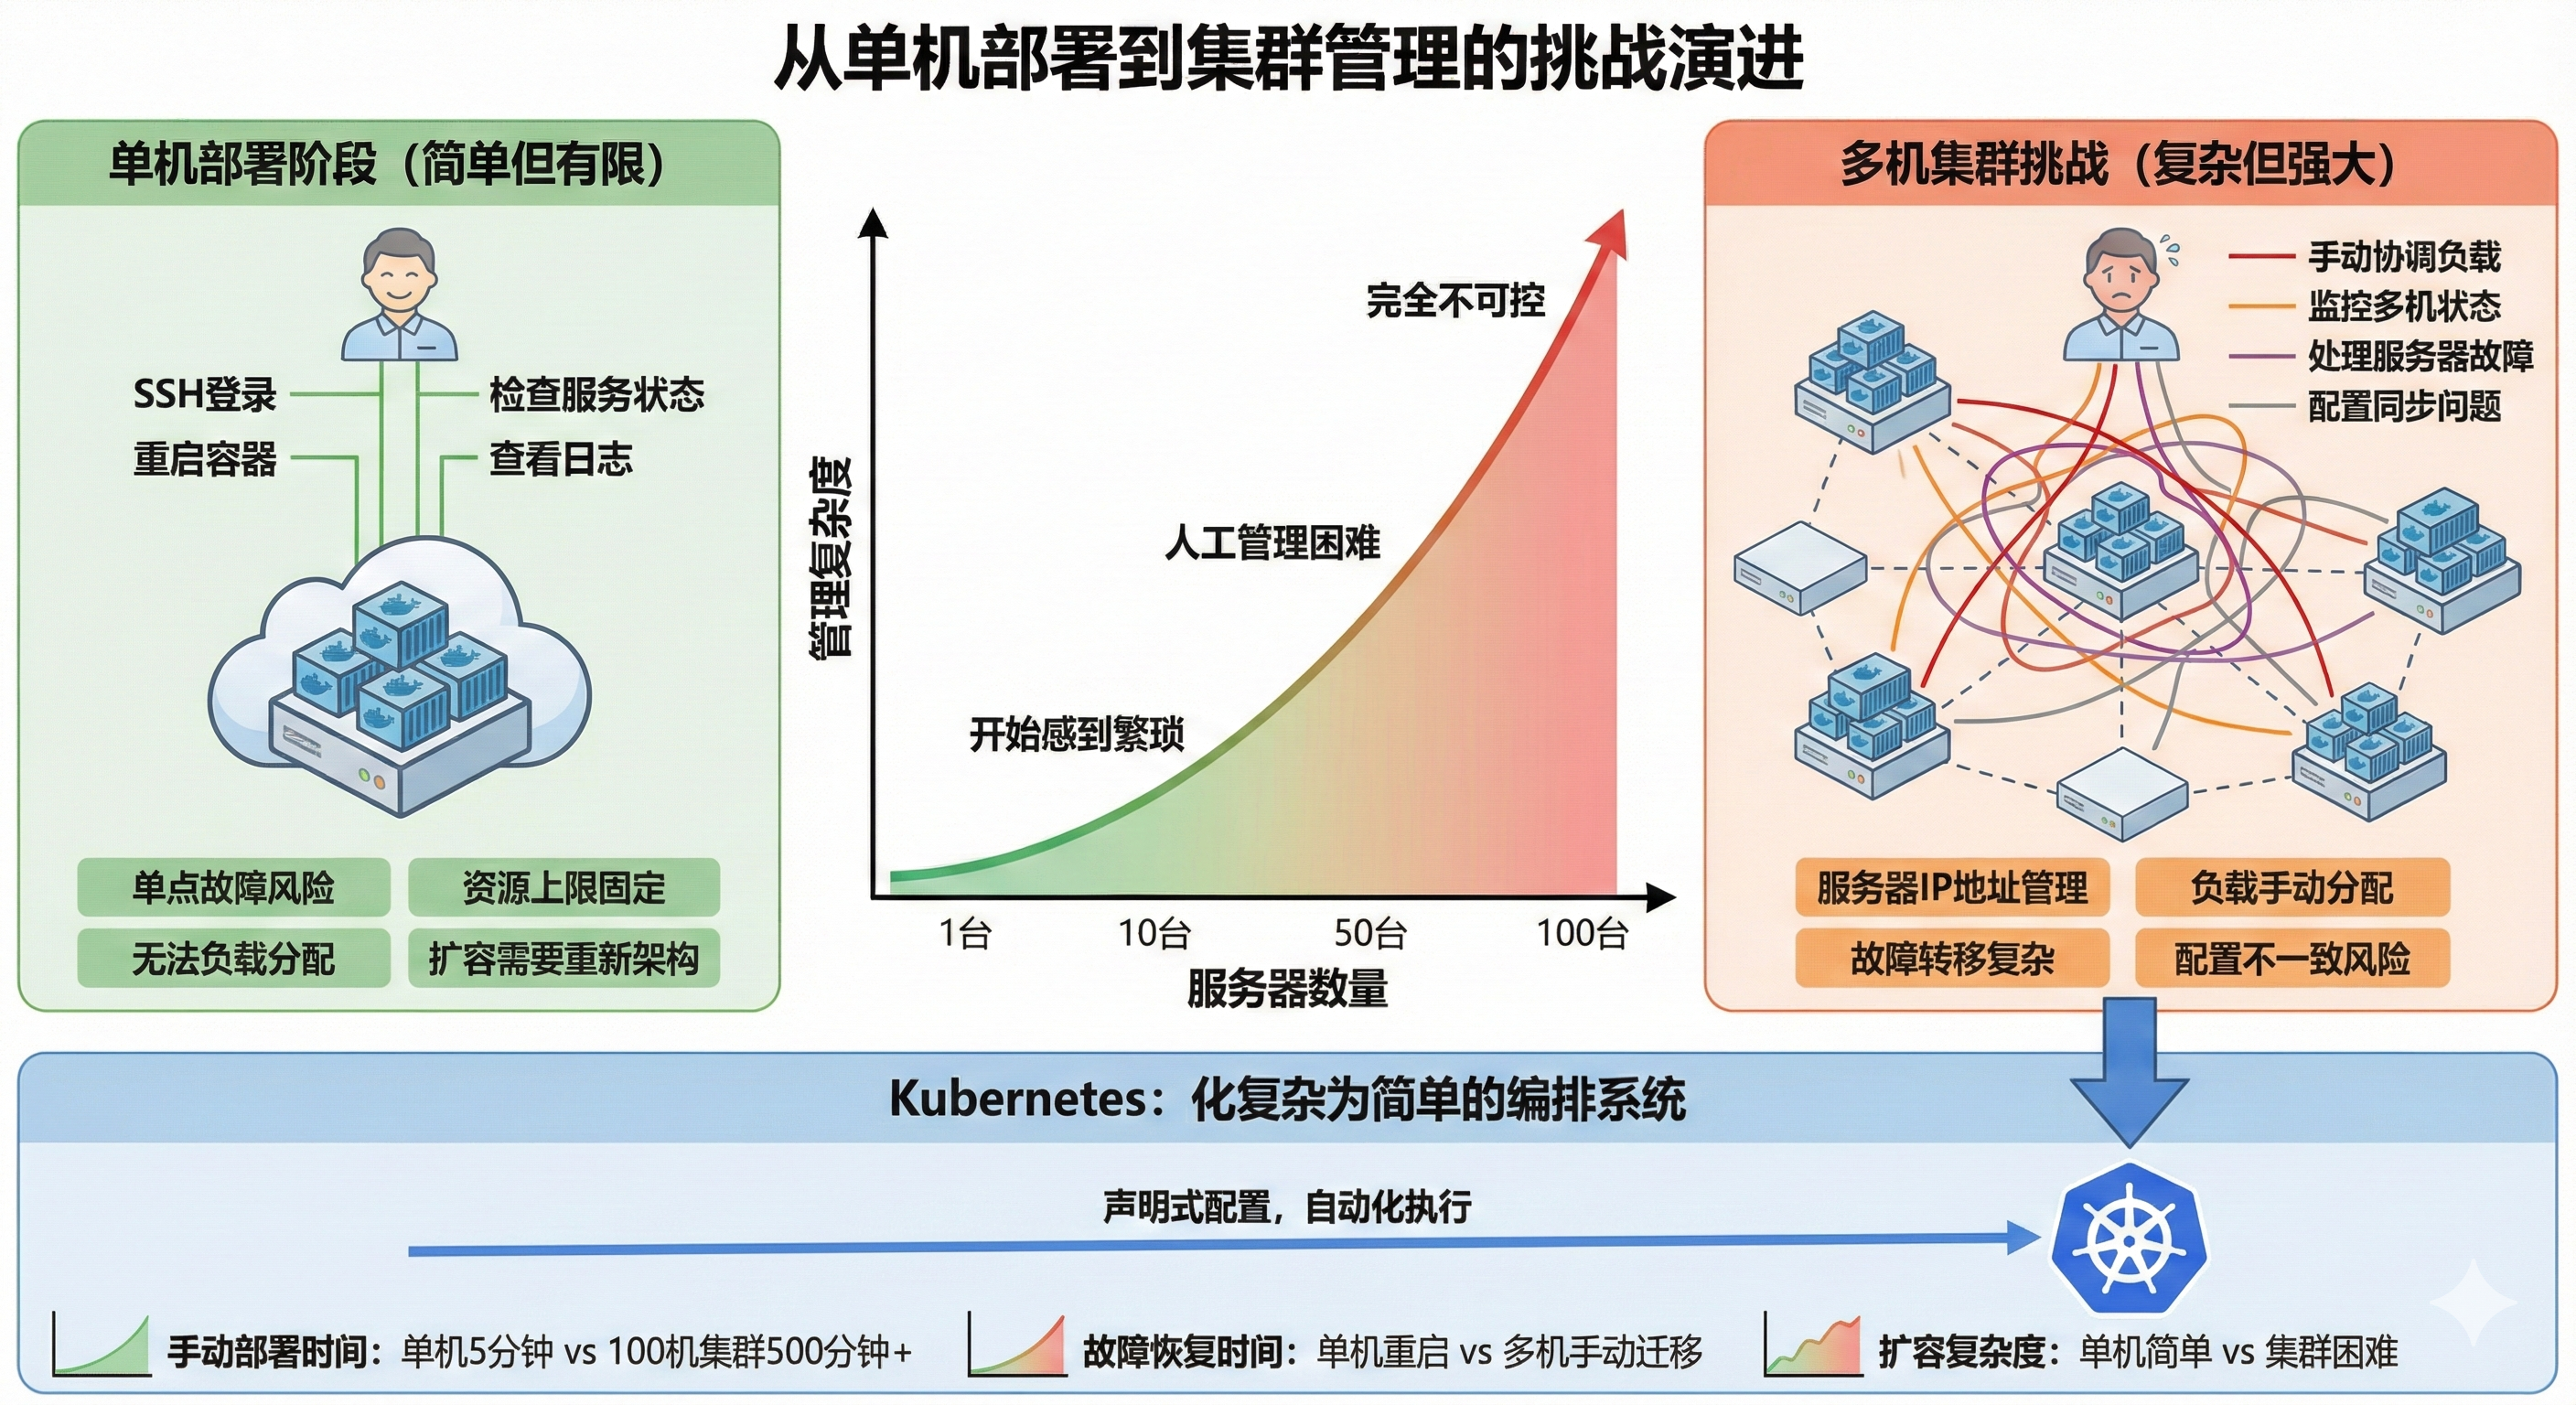
\includegraphics[width=0.9\textwidth]{figures/sec5/single-server-vs-cluster-management.png}
\caption{从单机部署到集群管理的挑战演进}
\label{fig:single-vs-cluster}
\end{figure}

如图\ref{fig:single-vs-cluster}所示，从单机部署向多机集群的扩展过程中，管理复杂度呈指数级增长，而Kubernetes正是为了解决这个根本性挑战而诞生的。

\subsubsection{Kubernetes：分布式系统的大脑}

Kubernetes（简称K8s）本质上是一个分布式的容器编排系统，但更准确地说，它是一个"分布式系统的操作系统"。如果把传统的操作系统比作管理单台计算机上各种程序运行的管家，那么Kubernetes就是管理整个数据中心中成千上万个容器协同工作的超级管家。

这个"超级管家"的核心价值在于将复杂的分布式系统管理抽象为简单的声明式操作。你不需要关心具体在哪台机器上运行什么容器，也不需要手动处理服务器故障和负载均衡，只需要告诉Kubernetes"我需要运行什么服务，需要多少个副本，需要什么样的资源"，它就会自动协调整个集群来实现你的期望。

Kubernetes的工作原理可以类比为一个拥有全局视野的智能调度中心。它持续监控整个集群中每台服务器的资源使用情况、每个容器的健康状态、每个服务的负载情况，然后基于这些信息做出智能的调度决策。当需要启动新容器时，它会选择最合适的服务器；当某台服务器过载时，它会自动将部分容器迁移到其他服务器；当某个容器崩溃时，它会立即在其他地方启动替代容器。

更重要的是，Kubernetes采用了"声明式"而非"命令式"的管理哲学。传统的运维方式是命令式的：你需要明确告诉系统执行每一个具体步骤，比如"在服务器A上启动容器X，在服务器B上启动容器Y，配置负载均衡器指向这两个容器"。而Kubernetes的声明式方式让你只需要描述期望的最终状态："我需要3个游戏服务器容器在运行，每个容器分配512MB内存"，然后K8s会自动分析当前状态与期望状态的差异，并执行必要的操作来达成目标。

\begin{figure}[htbp]
\centering
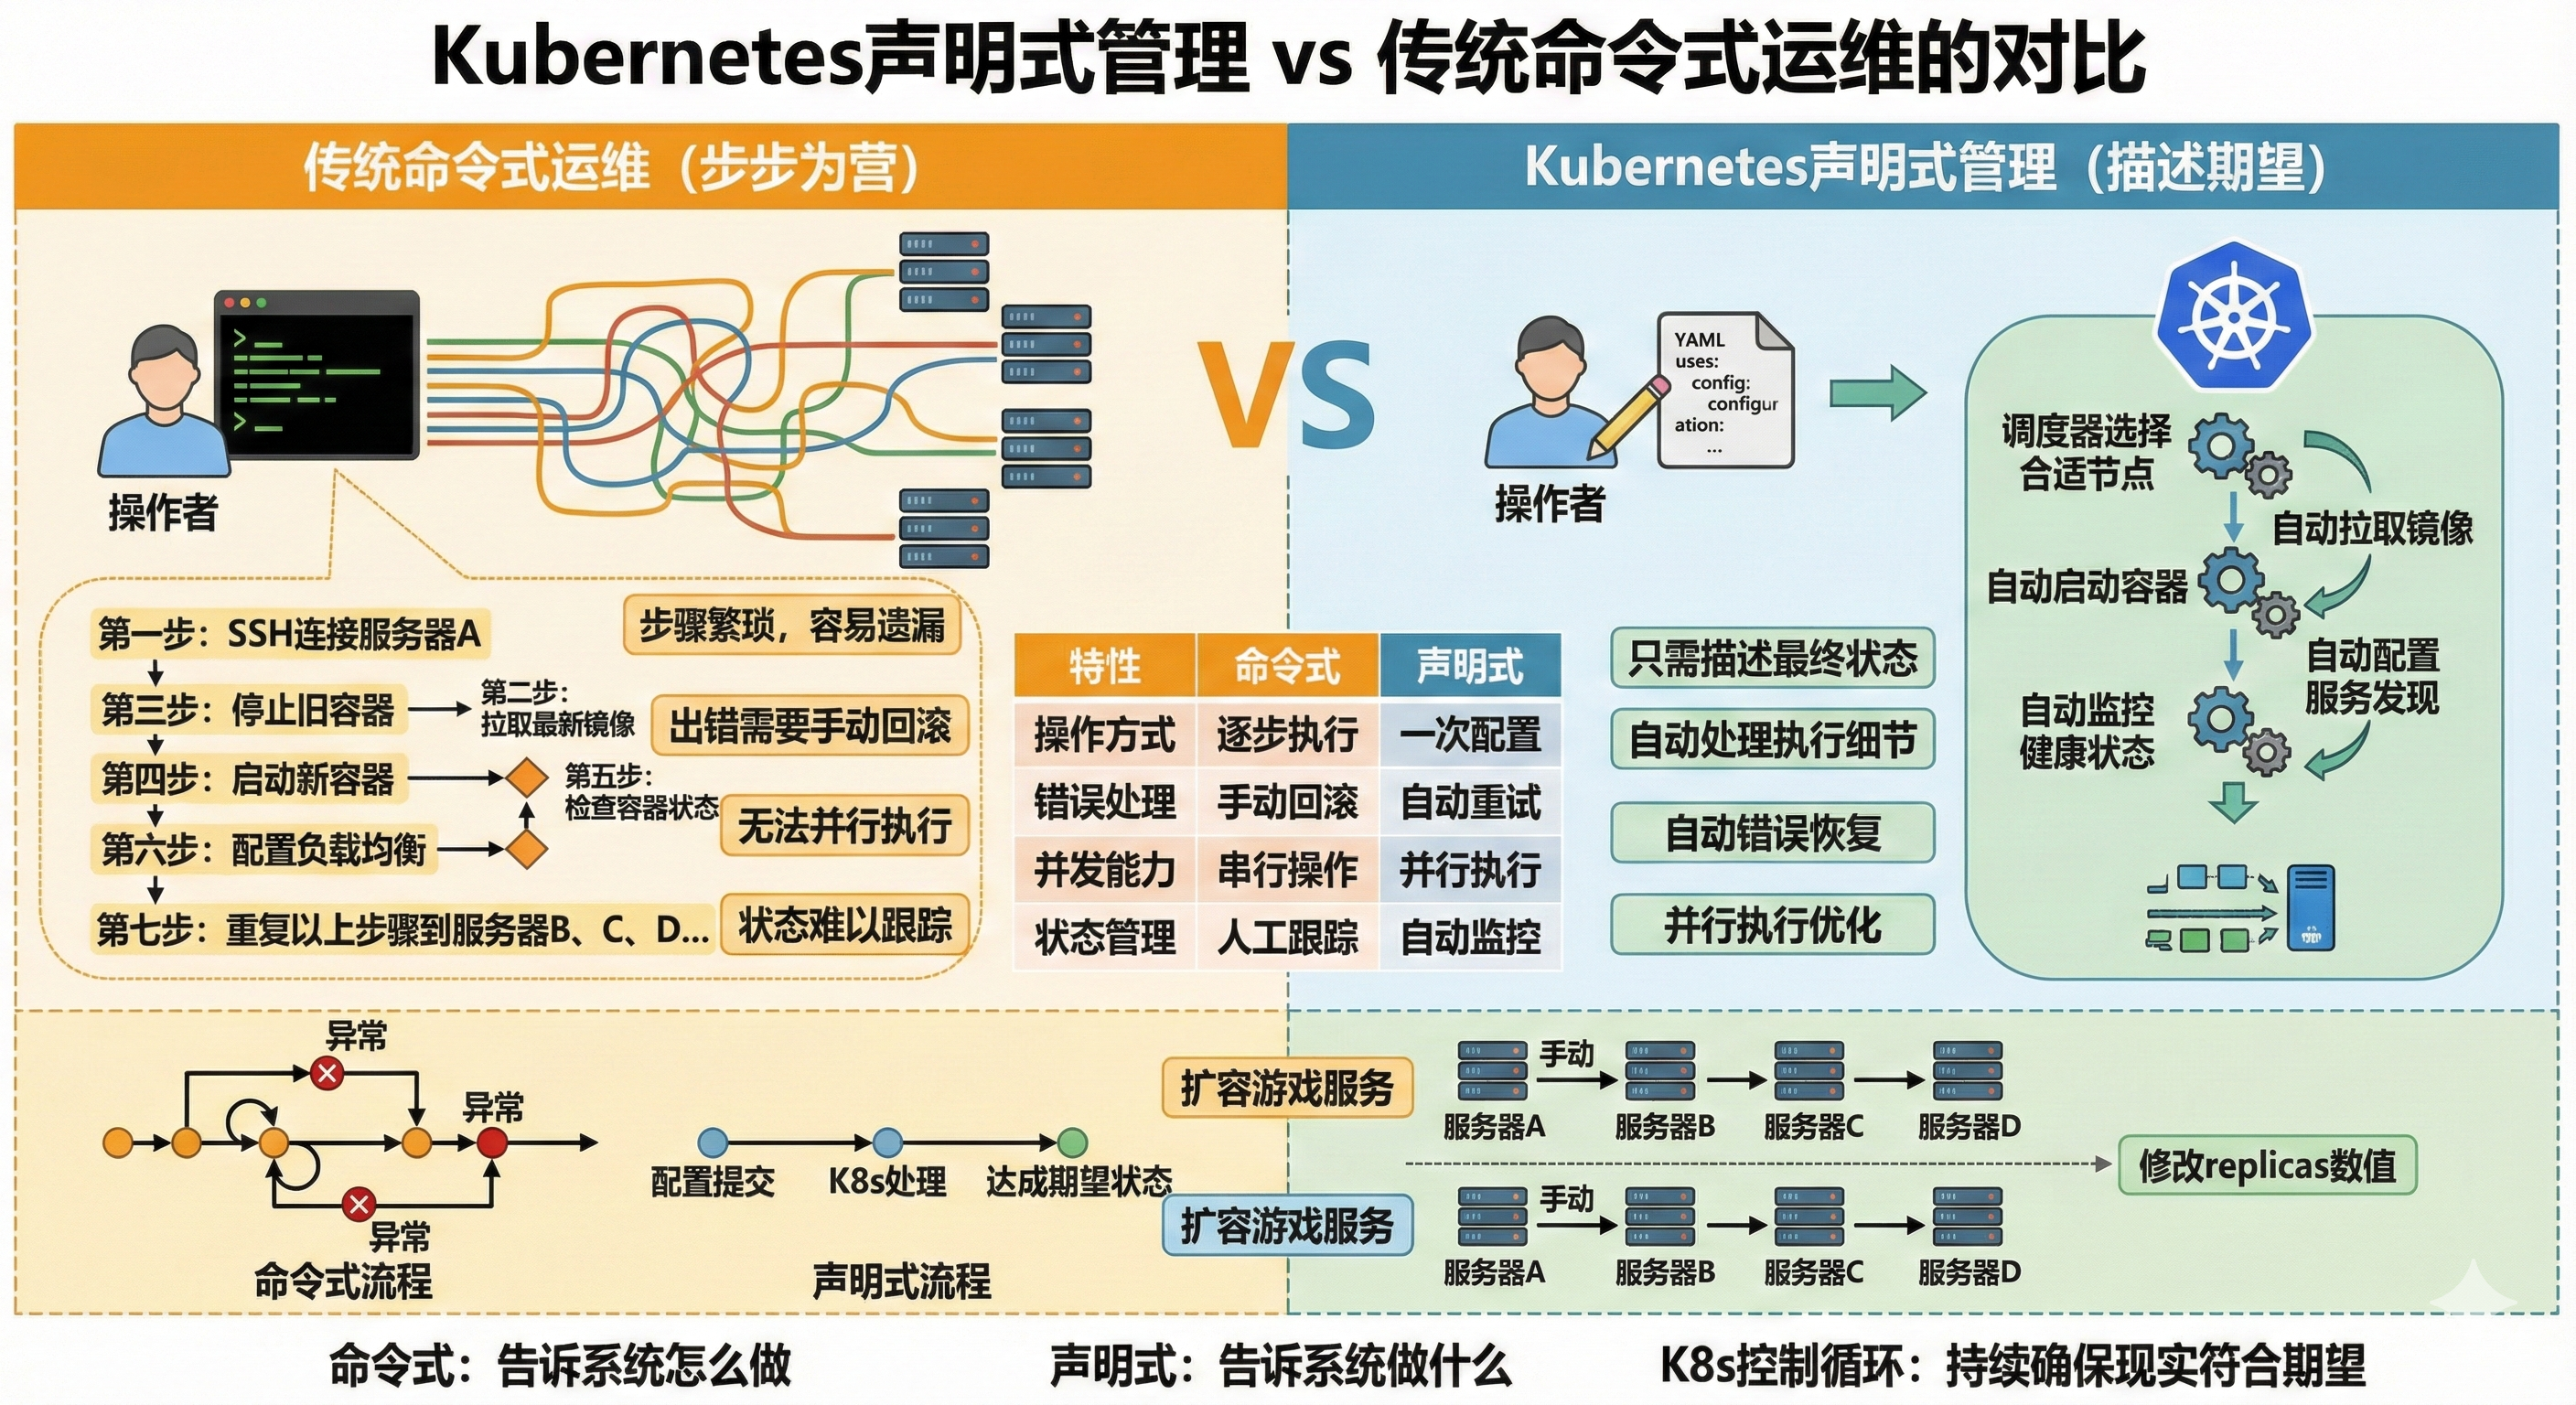
\includegraphics[width=0.9\textwidth]{figures/sec5/kubernetes-declarative-vs-imperative.png}
\caption{Kubernetes声明式管理 vs 传统命令式运维的对比}
\label{fig:declarative-vs-imperative}
\end{figure}

如图\ref{fig:declarative-vs-imperative}所示，这种声明式的设计哲学带来了巨大的运维效率提升。当你需要扩容时，只需要修改"期望副本数"这一个数字，K8s会自动处理后续的所有复杂操作；当你需要更新服务版本时，只需要修改镜像版本号，K8s会自动执行滚动更新，确保服务不中断；当某台服务器需要维护时，K8s会自动将其上的容器迁移到其他服务器，实现零停机维护。

\subsubsection{核心概念：K8s世界的组织架构}

要掌握Kubernetes，必须理解它的几个核心概念。这些概念构成了K8s管理容器化应用的基础框架，我们可以将其类比为一个现代化工厂的组织结构来理解。

\textbf{Cluster（集群）}是整个Kubernetes系统的边界，代表了所有被统一管理的计算资源的集合。就像一个工业园区包含了多个厂房、办公楼、仓库等设施一样，一个K8s集群包含了多台服务器、网络设备、存储系统等基础设施。集群提供了统一的资源池和管理界面，让运维人员可以将分散的硬件资源作为一个整体来使用。

\textbf{Node（节点）}是集群中的单台物理服务器或虚拟机，相当于工厂中的一个车间。每个Node都具备独立的计算、存储和网络能力，是承载实际工作负载的基础单元。Kubernetes的控制平面会持续监控每个Node的资源使用情况、健康状态，并根据这些信息做出智能的调度决策。当某个Node出现故障时，K8s会自动将其上的工作负载迁移到健康的Node上，确保服务不中断。

\textbf{Pod（容器组）}是Kubernetes中最小的部署和管理单元。一个Pod通常包含一个主要的应用容器和若干个辅助容器，它们共享网络和存储资源，必须被调度到同一个Node上一起运行。可以将Pod理解为车间里的一个工作小组，小组内的工人（容器）需要紧密协作，共享相同的工作环境。对于我们的游戏服务，一个Pod通常包含一个游戏服务器容器，以及可能的日志收集或监控辅助容器。

\textbf{Deployment（部署控制器）}负责管理Pod的生命周期，确保始终有期望数量的Pod实例在健康运行。它就像工厂里的生产主管，负责监督工作小组的数量和状态。如果某个Pod因为故障下线，Deployment会自动创建新的Pod替换；如果需要扩容，Deployment会启动更多Pod副本；如果需要更新服务版本，Deployment会协调滚动更新过程，确保服务连续性。

\textbf{Service（服务抽象）}为一组功能相同的Pod提供统一的访问入口和负载分发机制。它就像工厂的客服中心，外部客户无需知道具体哪个工作小组在处理自己的订单，只需要联系客服中心，Service会自动将请求分配给可用的Pod。Service还提供了服务发现功能，让不同的服务可以通过稳定的名称相互找到，而不用关心底层Pod的具体位置和IP地址。

\begin{figure}[htbp]
\centering
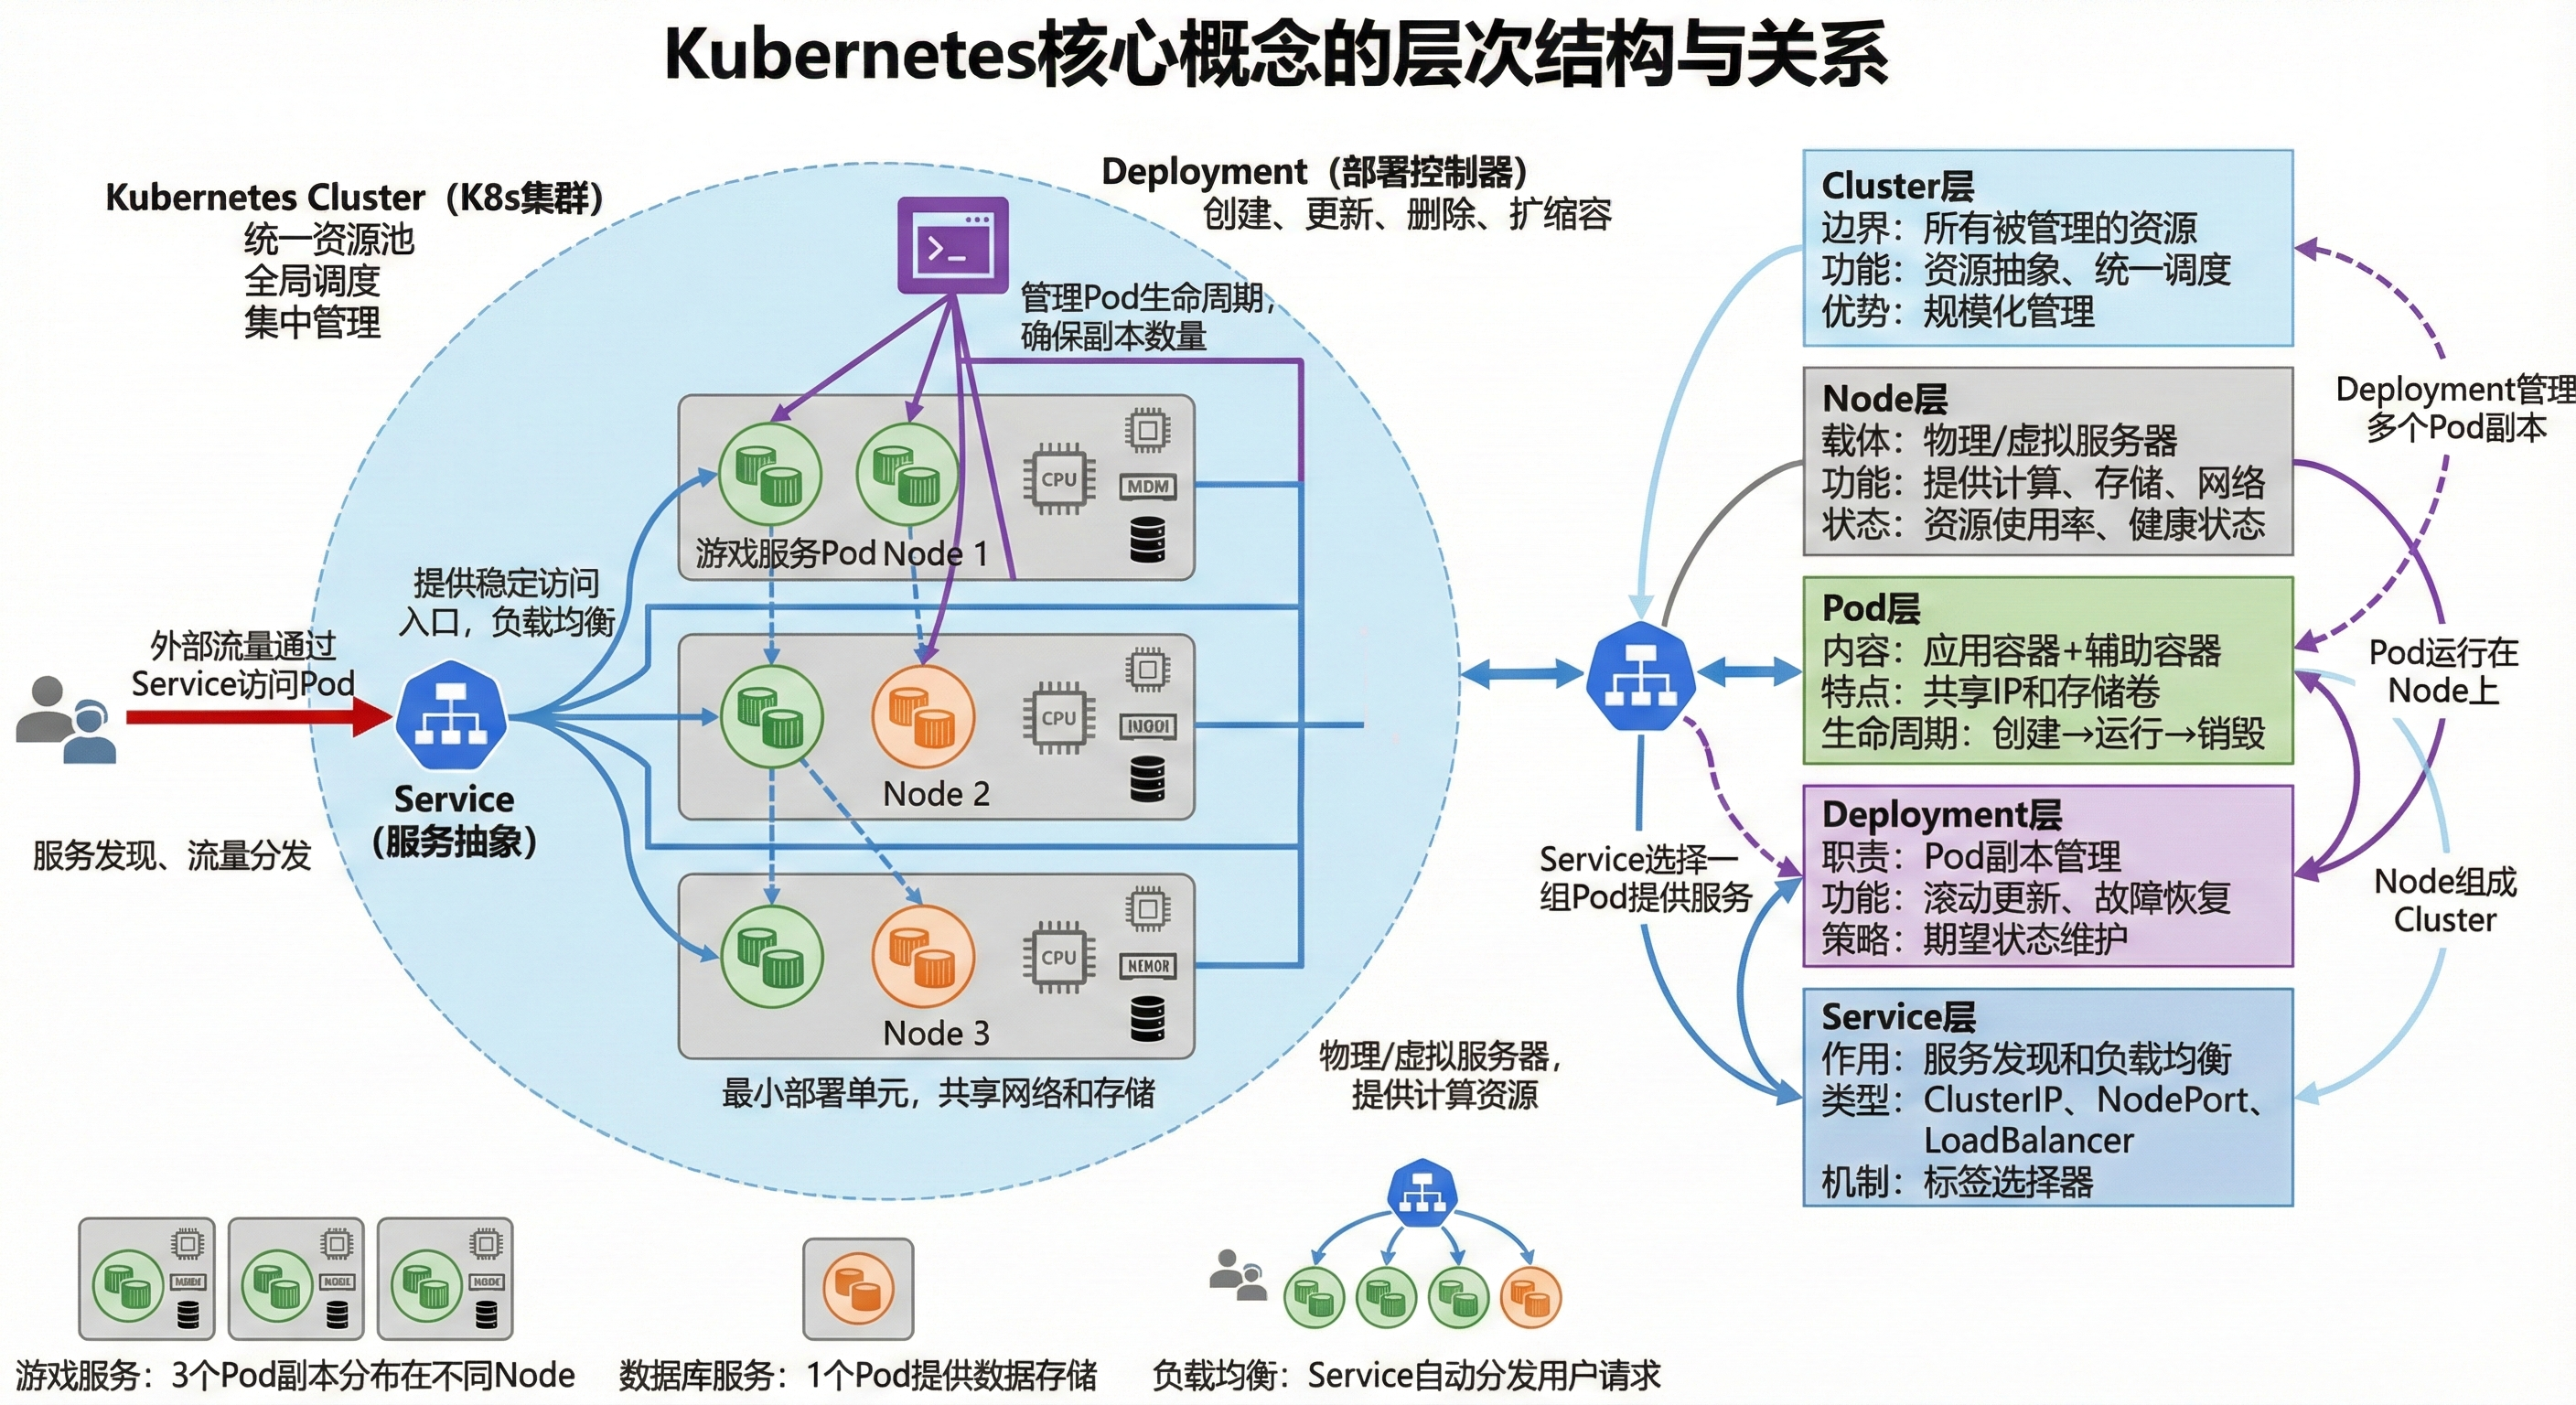
\includegraphics[width=0.9\textwidth]{figures/sec5/kubernetes-architecture-concepts.png}
\caption{Kubernetes核心概念的层次结构与关系}
\label{fig:k8s-concepts}
\end{figure}

如图\ref{fig:k8s-concepts}所示，这些概念形成了一个完整的层次化架构：Cluster提供资源边界，Node提供计算载体，Pod承载应用实例，Deployment管理Pod生命周期，Service提供访问入口，共同构成了Kubernetes强大的容器编排能力。

\subsubsection{工作流程：从配置到运行的自动化魔法}

了解了核心概念后，让我们深入了解Kubernetes是如何将我们的期望转化为实际运行的服务的。整个过程体现了现代云原生系统"配置驱动、自动执行"的设计理念。

当我们提交一份Deployment配置时，实际上是在向Kubernetes描述一个期望状态：我们希望有多少个Pod在运行，每个Pod使用什么镜像，需要多少资源等等。Kubernetes的控制循环（Control Loop）会持续比较当前实际状态与期望状态，并自动执行必要的操作来消除差异。

这个过程的第一步是调度（Scheduling）。Kubernetes的调度器会分析每个新Pod的资源需求，然后在整个集群中寻找最合适的Node。调度算法会考虑多种因素：Node的剩余资源是否足够、是否有特殊的亲和性要求、是否需要避免某些Node等。调度决策完成后，kubelet（运行在每个Node上的代理程序）会接收指令并在本地启动相应的容器。

第二步是服务注册与发现。当Pod成功启动后，它会自动注册到相应的Service中。Service通过标签选择器（Label Selector）机制找到属于它的Pod，并将这些Pod的IP地址加入到负载均衡池中。这个过程是完全自动的，新启动的Pod会立即开始接收外部请求，下线的Pod会立即从负载均衡池中移除。

第三步是持续监控与自愈。Kubernetes会持续监控每个Pod的健康状态，通过健康检查（Health Check）机制检测Pod是否正常工作。如果发现Pod异常，Deployment控制器会立即启动新的Pod来替换故障实例。这种自愈能力让系统具备了很强的容错性，单个Pod的故障不会影响整体服务的可用性。

\begin{figure}[htbp]
\centering
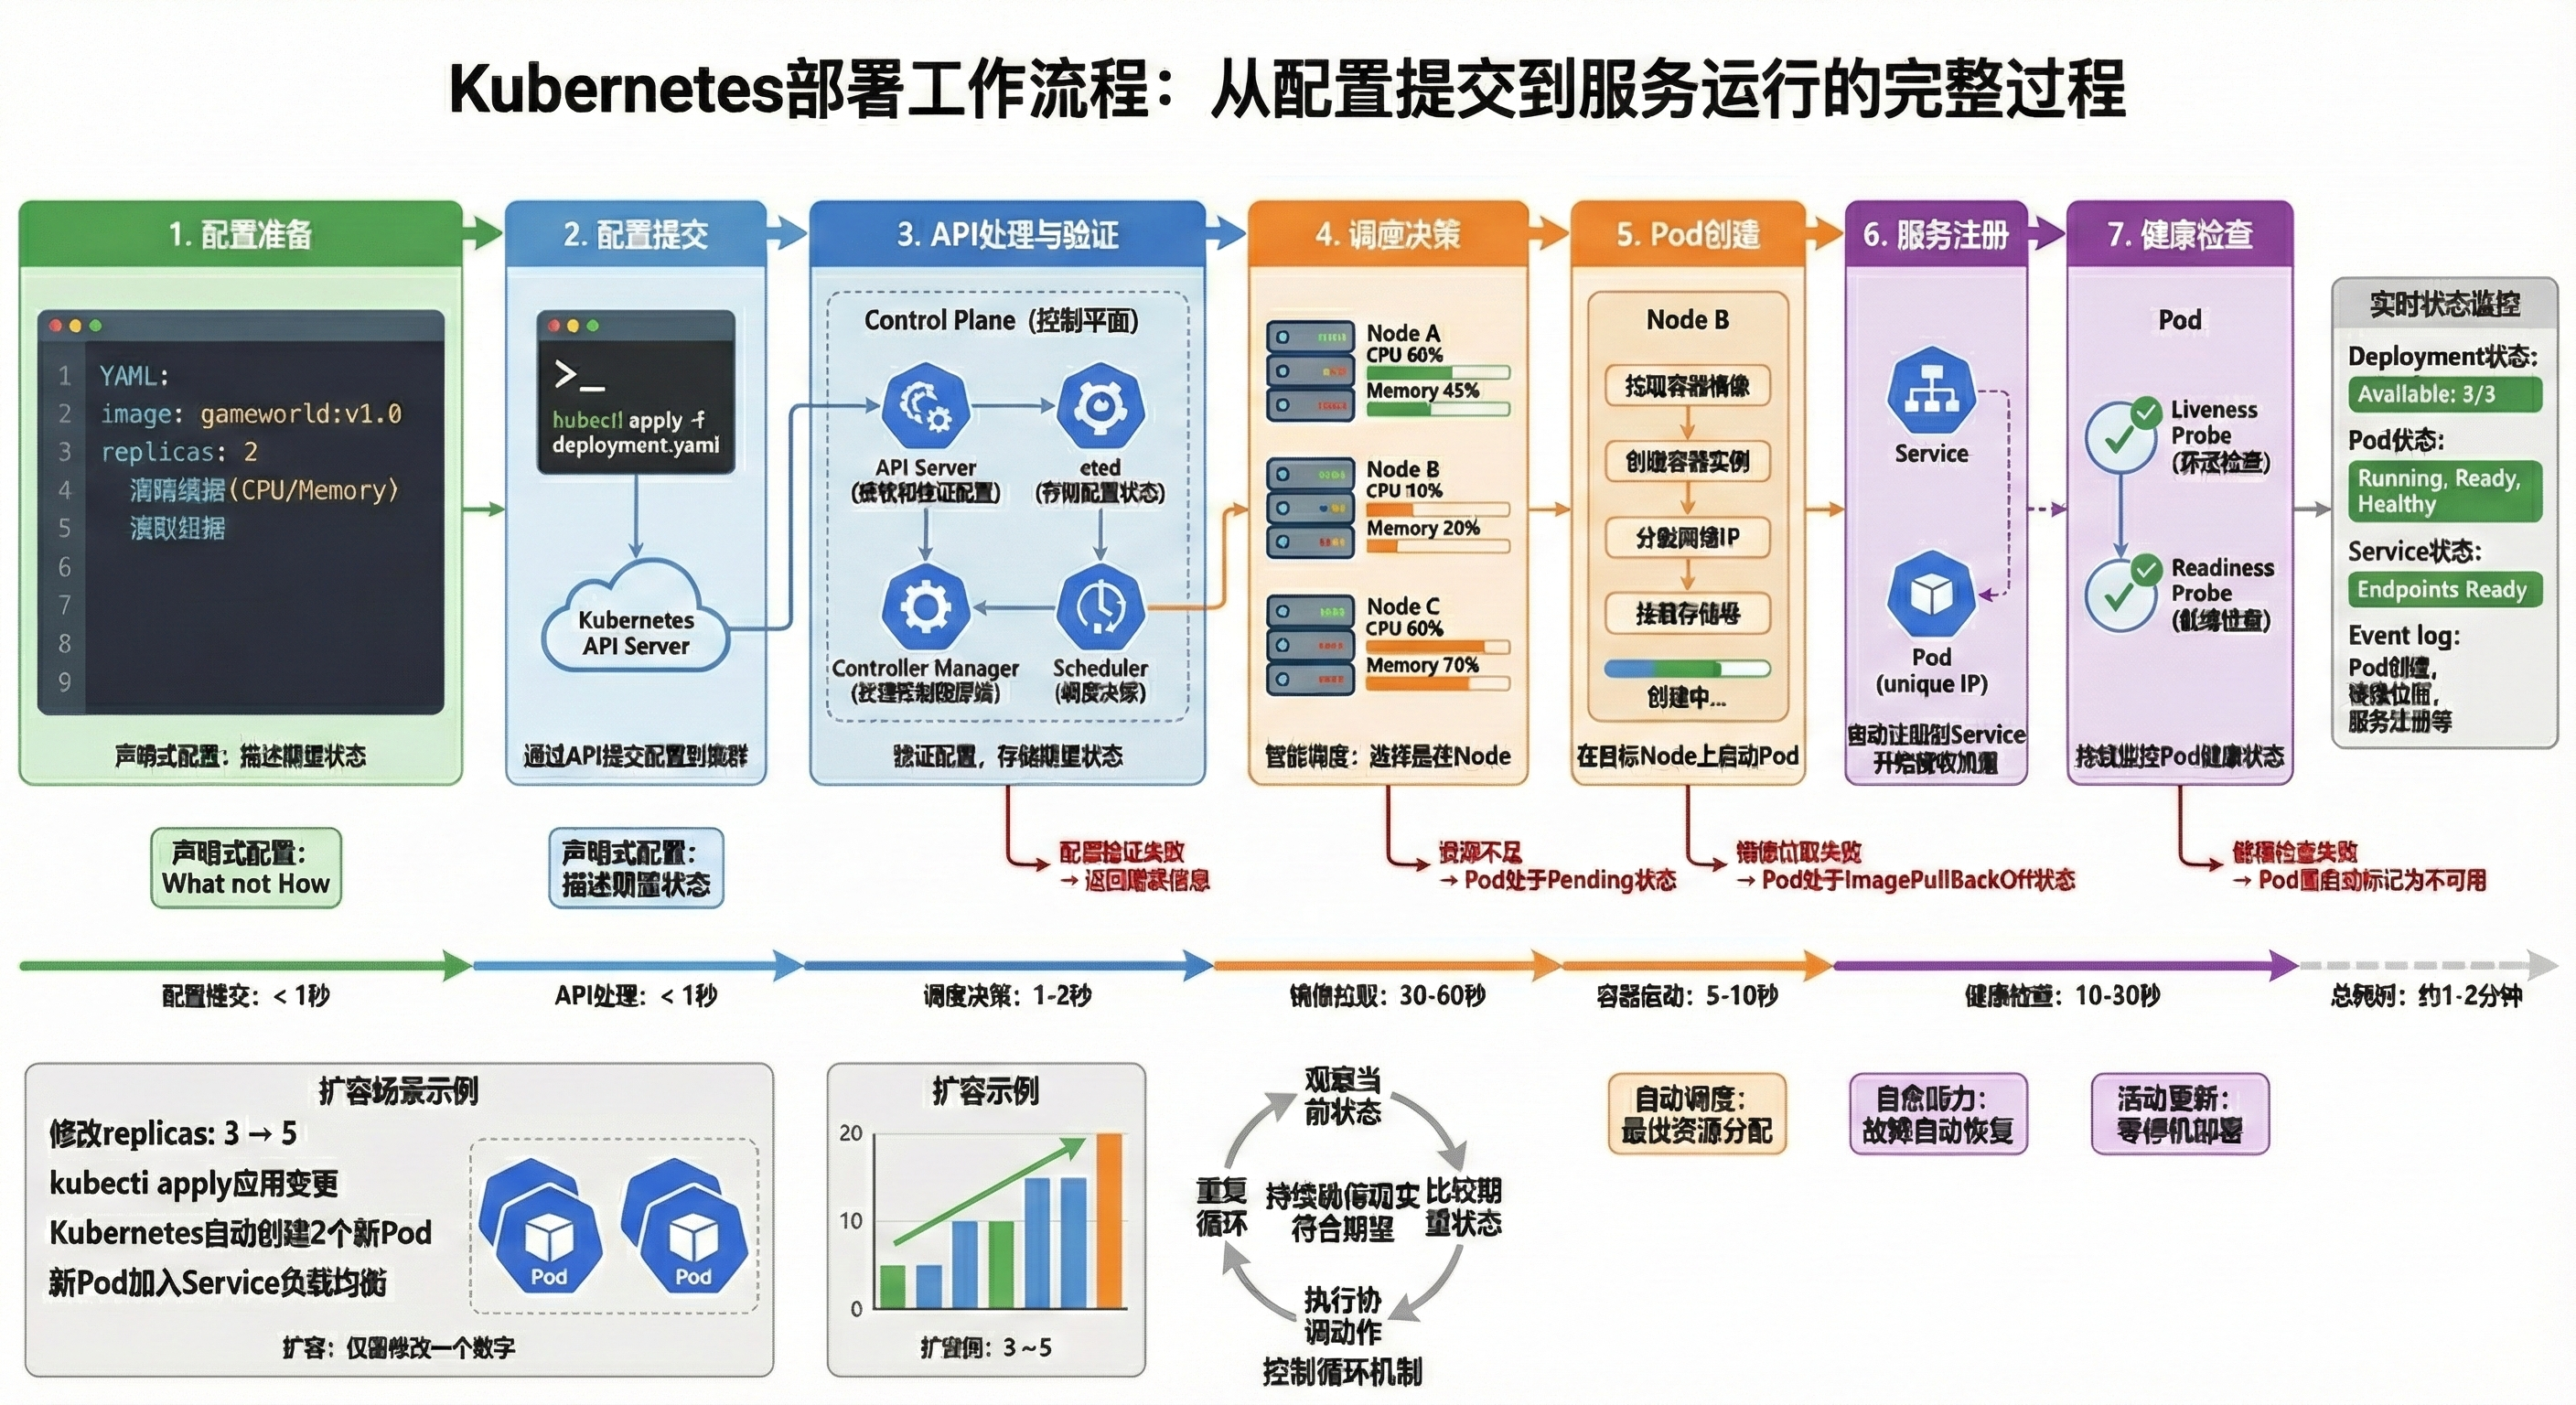
\includegraphics[width=0.9\textwidth]{figures/sec5/kubernetes-deployment-workflow.png}
\caption{Kubernetes部署工作流程：从配置提交到服务运行的完整过程}
\label{fig:k8s-workflow}
\end{figure}

如图\ref{fig:k8s-workflow}所示，最令人印象深刻的是扩容过程的简化。当我们需要应对流量增长时，只需要修改Deployment配置中的副本数（replicas），K8s就会自动启动新的Pod实例。调度器会选择合适的Node，kubelet会拉取镜像并启动容器，Service会自动将新Pod加入负载均衡，整个过程无需人工干预，通常在几分钟内就能完成。

\subsubsection{实战演练：将游戏服务托管给K8s}

理解了Kubernetes的工作原理后，让我们通过实际的部署过程来体验其强大能力。整个部署过程体现了"声明期望，自动实现"的云原生理念。

部署准备的第一步是确保镜像资源就绪。我们需要将游戏服务的Docker镜像推送到Kubernetes集群可以访问的镜像仓库中。这个步骤延续了我们在容器化阶段建立的标准化流程，确保集群中的任何Node都能获取到相同的镜像版本。

第二步是编写声明式配置文件。Kubernetes使用YAML格式的配置文件来描述期望状态，这些配置文件包含了资源定义、依赖关系、约束条件等所有必要信息。对于我们的游戏服务，主要需要定义Deployment和Service两类资源。

\begin{figure}[htbp]
\centering
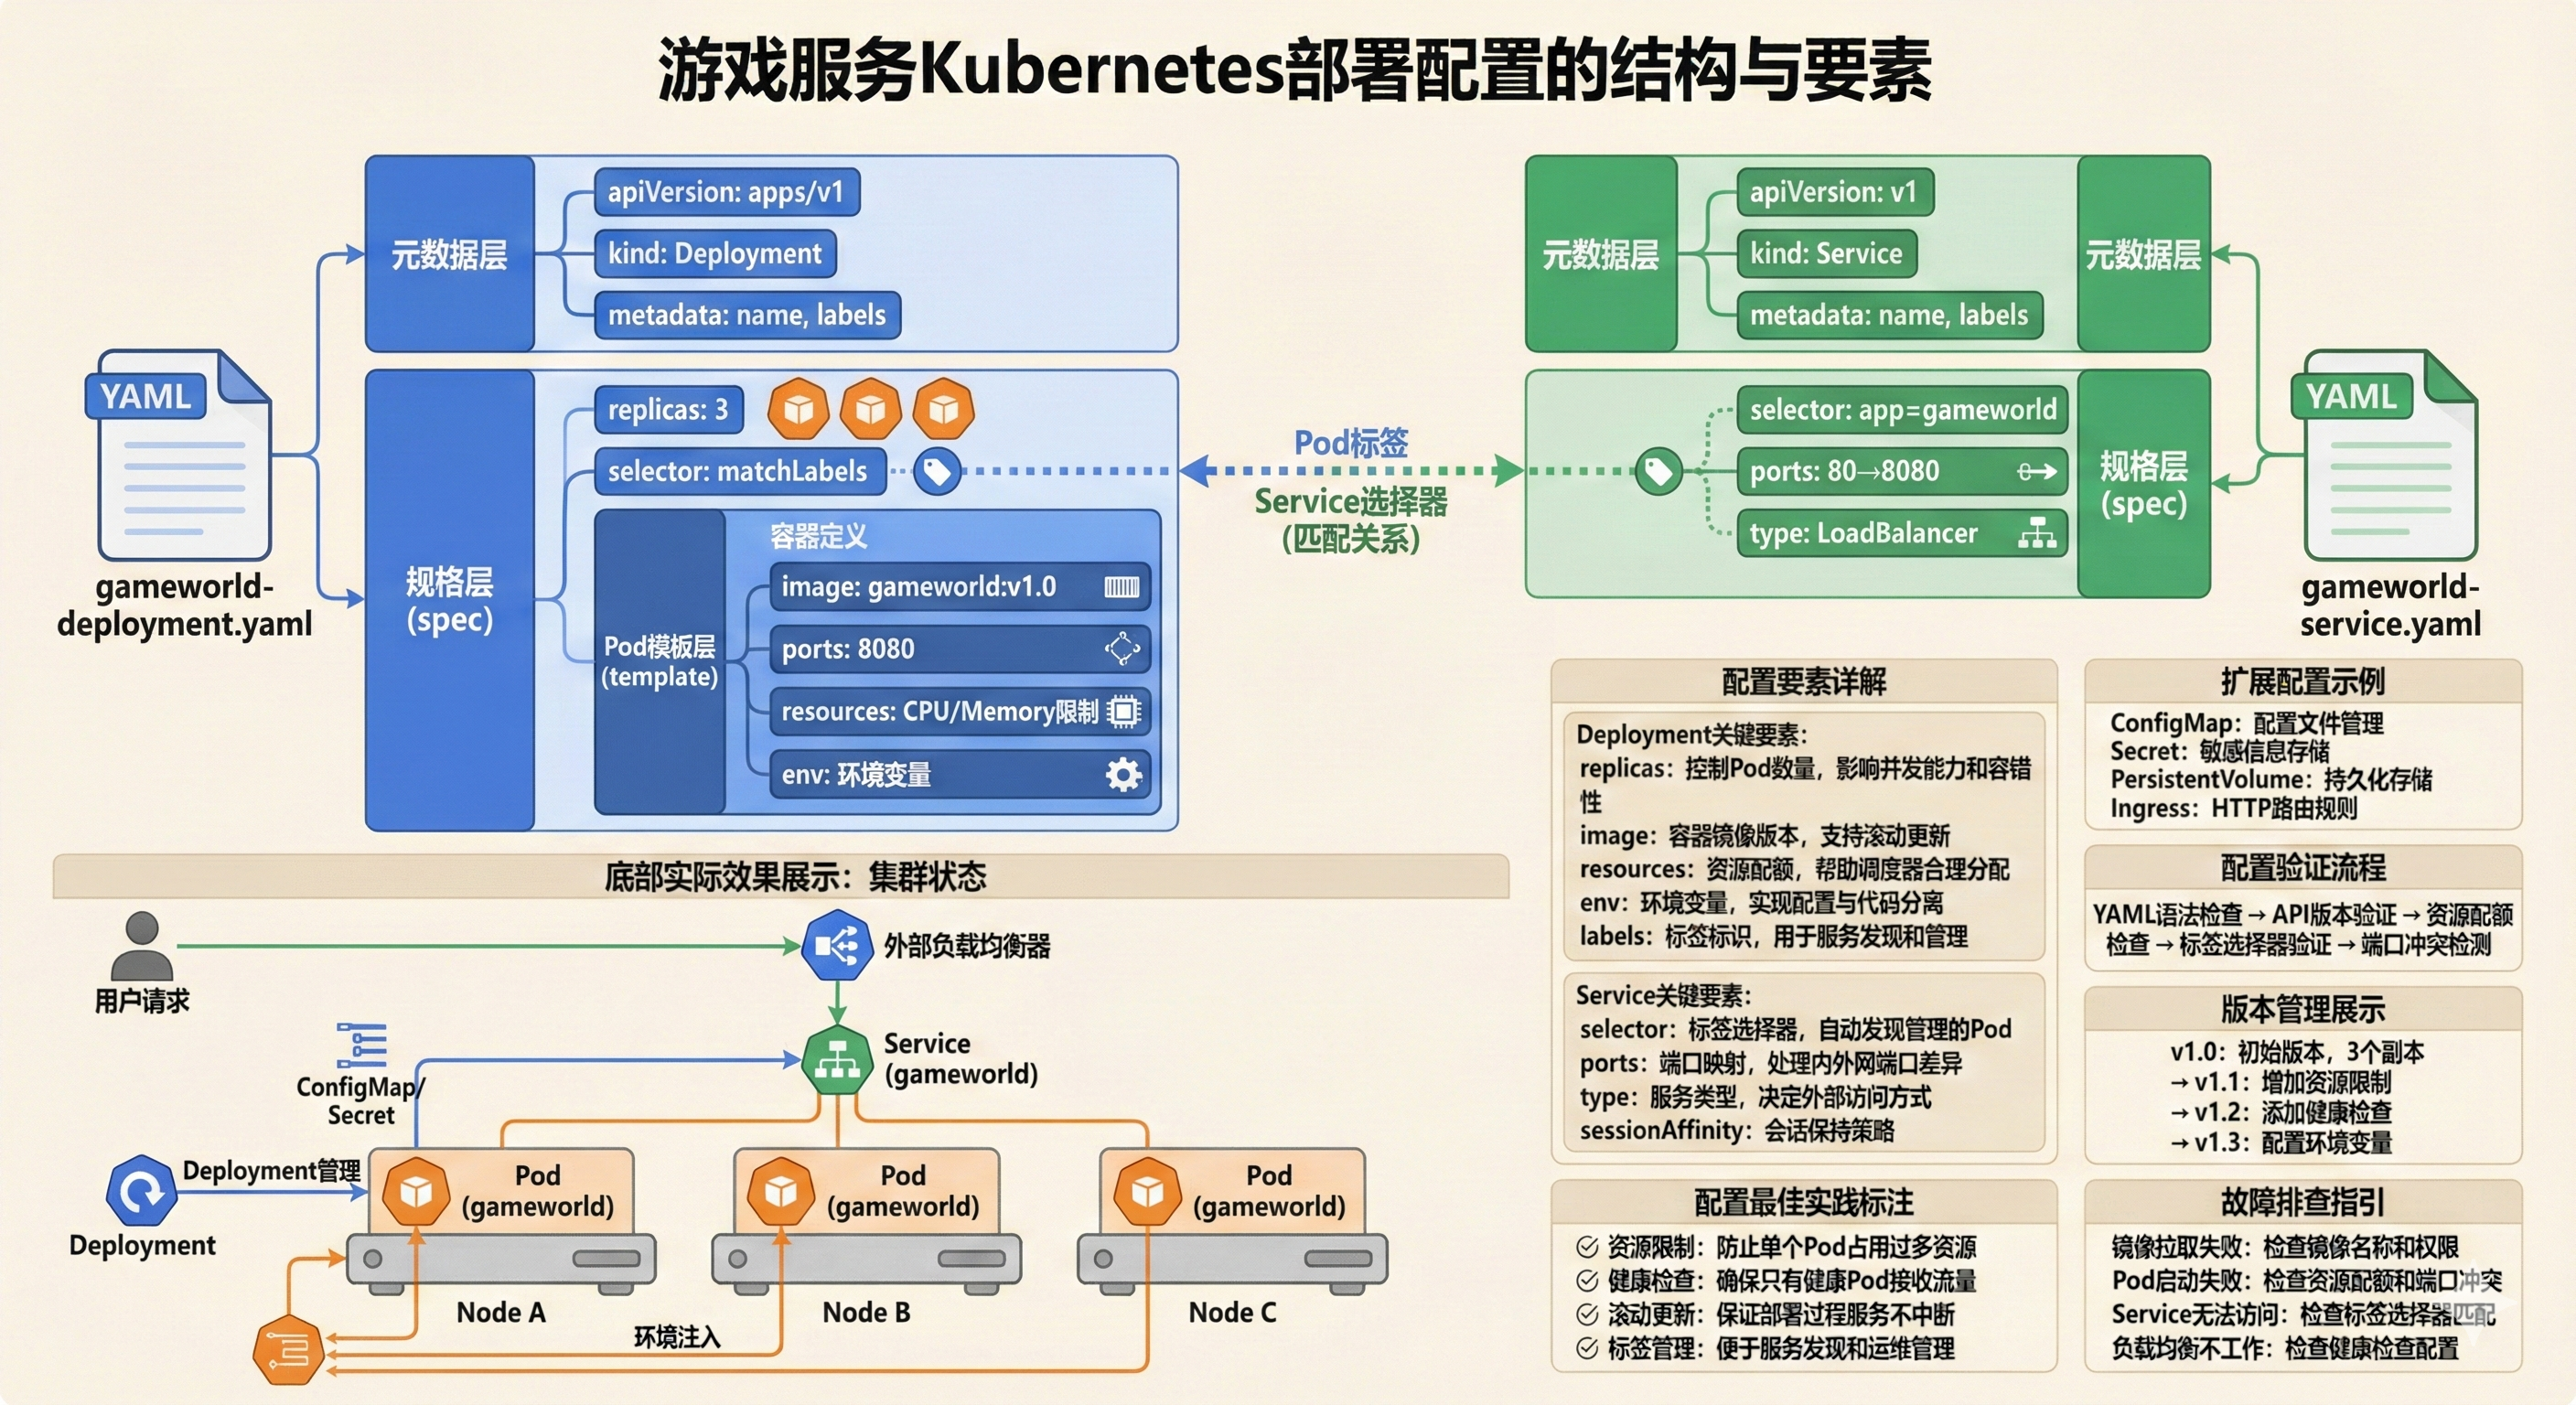
\includegraphics[width=0.9\textwidth]{figures/sec5/kubernetes-deployment-configuration.png}
\caption{游戏服务Kubernetes部署配置的结构与要素}
\label{fig:k8s-config}
\end{figure}

如图\ref{fig:k8s-config}所示，Deployment配置定义了Pod模板、副本数量、更新策略、资源限制等关键参数。副本数量决定了系统的并发处理能力和容错级别；资源限制帮助调度器进行合理的资源分配；更新策略确保版本升级时的服务连续性。这种配置方式将复杂的运维决策转化为了清晰的参数设置，大大降低了出错的可能性。

Service配置定义了服务的网络暴露方式、端口映射、负载均衡策略等。通过标签选择器机制，Service能够自动发现并管理所有相关的Pod，形成统一的访问入口。负载均衡器的自动配置让外部流量能够均匀分配到所有健康的Pod实例上，实现了高可用和高性能。

第三步是执行部署命令。通过kubectl命令行工具，我们可以将配置文件提交给Kubernetes API服务器。一旦配置被接受，整个集群就会开始协调工作来实现期望状态。我们可以通过各种kubectl命令来监控部署进度、查看资源状态、调试问题。

\begin{figure}[htbp]
\centering
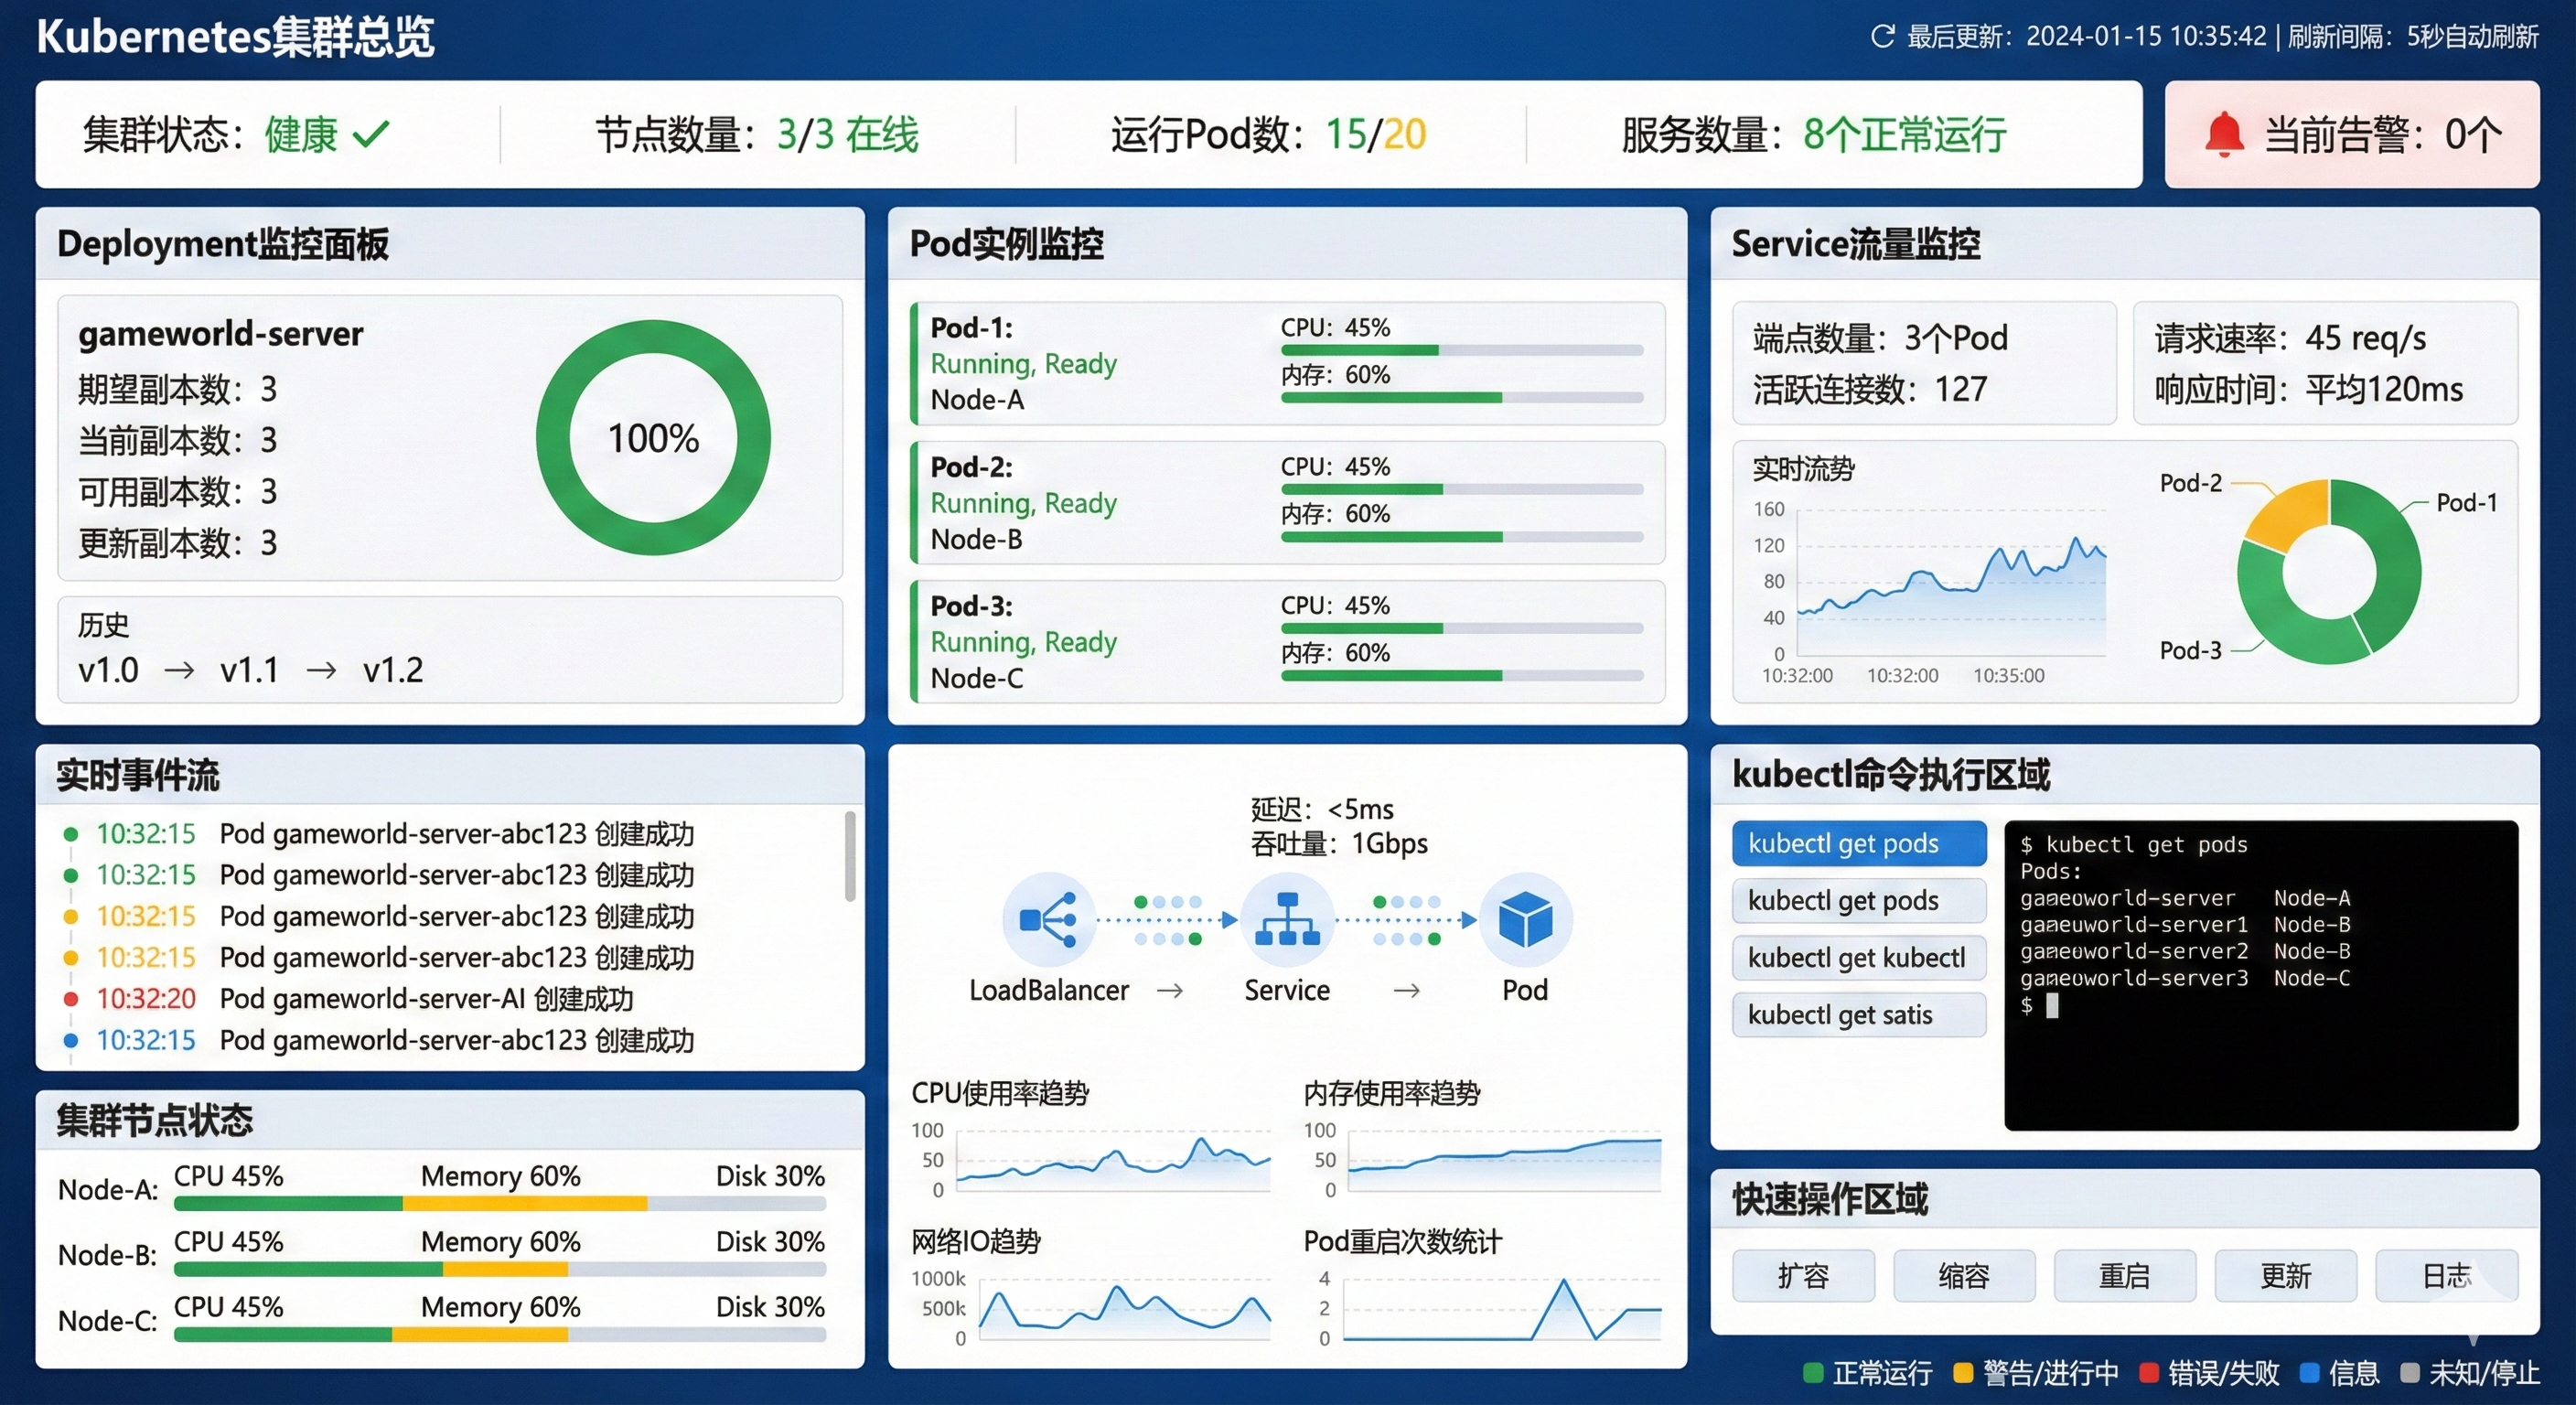
\includegraphics[width=0.9\textwidth]{figures/sec5/kubernetes-deployment-monitoring.png}
\caption{Kubernetes部署过程的监控与状态查看}
\label{fig:k8s-monitoring}
\end{figure}

如图\ref{fig:k8s-monitoring}所示，部署完成后，我们就获得了一个高度自动化的服务运行环境。当需要扩容时，只需修改配置文件中的副本数并重新应用；当需要更新服务版本时，只需修改镜像标签并执行滚动更新；当某个Pod出现故障时，Kubernetes会自动重启或替换。这种自动化程度让运维工作从"被动响应"转变为"主动配置"，大大提升了效率和可靠性。

通过这一节的学习，我们已经掌握了Kubernetes的核心理念和基本使用方法。但这仅仅是容器编排世界的入门，Kubernetes还提供了配置管理、服务网格、监控告警等更高级的功能。在接下来的章节中，我们将进一步探索如何利用这些高级特性构建真正的生产级系统。

当你看到kubectl命令返回"deployment successfully deployed"的提示时，意味着你已经成功将应用从单机模式升级到了分布式集群模式。此时的游戏服务不再依赖于单台服务器的稳定性，而是由整个Kubernetes集群的智能调度和自动恢复能力来保障，这是向云原生架构迈出的关键一步。




%\subsection{“弹性” 的奥义：迎接百万玩家的云端扩容术}
%\paragraph{本节目标} 理解弹性扩容，掌握 K8s 自动扩缩容逻辑。
%\paragraph{写作建议}
%\begin{enumerate}
%    \item 以 “固定服务器浪费 / 卡顿” 痛点，引出弹性（按负载调资源）。
%    \item 讲扩容逻辑：按 CPU 阈值（超 80\% 加 Pod，低于 30\% 减 Pod），Service 自动分请求。
%    \item 提 Node 扩容：Pod 不够时，云厂商自动加服务器。
%\end{enumerate}

\subsection{“弹性”的奥义：迎接百万玩家的云端扩容术}

\subsubsection{资源困境：当固定配置遇上波动流量}

在传统的服务器部署模式中，我们通常会基于业务高峰期的流量需求来配置服务器规格和数量。这种"按最坏情况准备"的策略虽然能够保证高峰期的服务质量，但却带来了严重的资源浪费问题。想象一下你经营着一家火爆的在线游戏：周五晚上8点，同时在线人数可能达到5万人，此时需要50台服务器才能保证流畅体验；而周二上午10点，在线人数可能只有5000人，理论上5台服务器就足够了。

这种资源配置困境的本质是"静态思维"与"动态现实"之间的根本矛盾。传统的IT架构假设负载是相对稳定和可预测的，因此采用了固定配置的设计思路。但互联网时代的业务负载具有强烈的波动性和不可预测性，这种静态配置必然导致要么资源过剩造成浪费，要么资源不足影响用户体验。

更深层的问题在于，互联网流量的波动模式远比我们想象的复杂。除了可以预见的周期性波动——工作日vs周末、白天vs夜晚、节假日效应等，还存在大量突发性和病毒式的流量爆炸。一个游戏主播的突然推荐、一次版本更新的Bug修复、一个网络热梗的病毒式传播，都可能在几分钟内让服务器负载暴增数十倍。

如果始终维持50台服务器运行，那么大部分时间里有90\%的计算资源在空转，每月产生巨额的无效成本。相反，如果为了节省成本而按照平均流量配置服务器，那么在流量高峰期就会出现严重的性能瓶颈。玩家会遭遇连接超时、操作卡顿甚至无法进入游戏等糟糕体验。这种"要么浪费钱，要么丢用户"的两难困境，是所有面向C端用户的互联网服务都必须面对的现实挑战。

\begin{figure}[htbp]
\centering
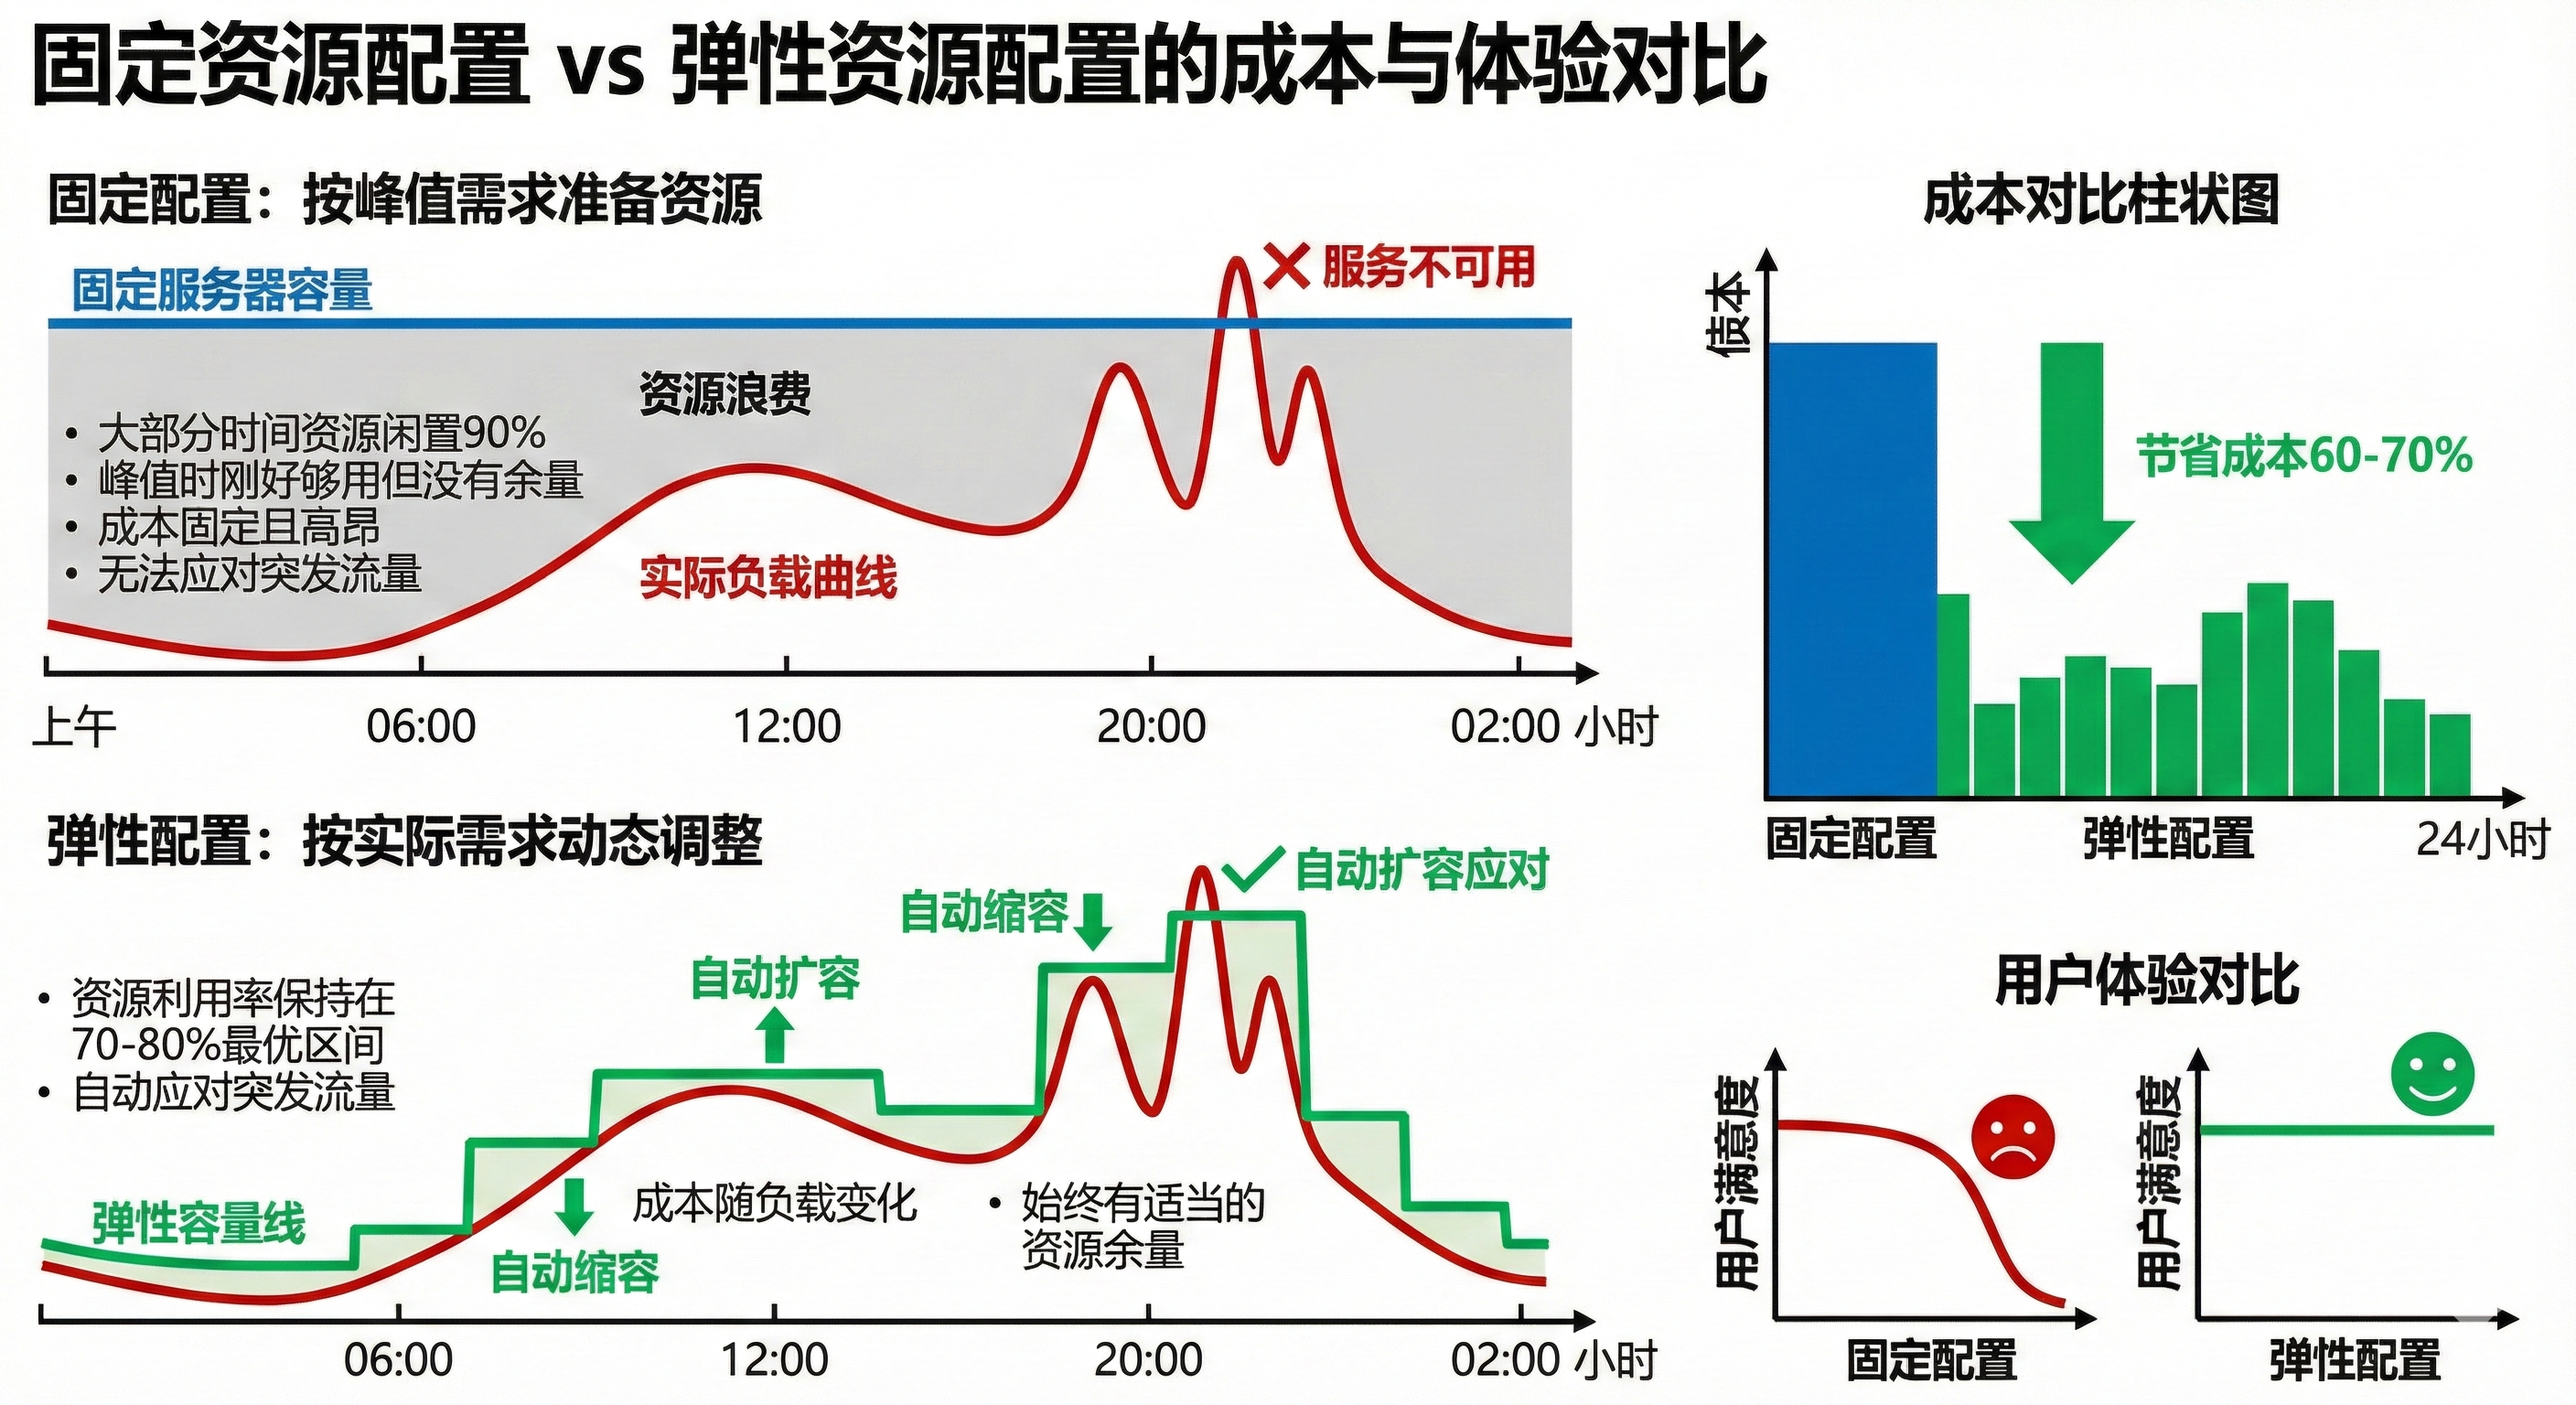
\includegraphics[width=0.9\textwidth]{figures/sec5/fixed-vs-elastic-resources.png}
\caption{固定资源配置 vs 弹性资源配置的成本与体验对比}
\label{fig:fixed-vs-elastic}
\end{figure}

如图\ref{fig:fixed-vs-elastic}所示，传统的固定配置模式在处理波动性负载时存在结构性缺陷，而弹性配置能够实现成本与性能的动态平衡。

\subsubsection{弹性扩容的核心思想：让资源像水一样流动}

"弹性扩容"的核心价值就是要彻底解决资源配置与流量波动之间的矛盾。它代表了一种全新的资源管理哲学：不再将服务器数量视为固定的静态配置，而是将其转变为根据实时负载动态调整的弹性变量。这种转变的意义远不止技术层面的优化，更是思维模式从"拥有资源"向"使用资源"的根本转变。

弹性扩容的工作原理可以类比为现代城市的交通管理系统。在交通高峰期，系统会自动调配更多的公交车上路、开放更多的车道、延长信号灯时间；在交通低峰期，则会减少运营车辆、关闭部分车道、缩短信号灯周期。这种动态调节不仅提升了整体效率，也避免了资源的无效占用。

在云计算环境中，弹性扩容通过持续监控关键指标（如CPU使用率、内存占用率、网络IO、响应时间等）来感知系统负载状态。当这些指标超过预设阈值时，系统会自动触发扩容操作：启动更多的服务实例、分配更多的计算资源、增加更多的服务器节点。当负载回落时，则执行相反的缩容操作，将多余的资源释放回资源池中供其他应用使用。

这种"按需分配，用完即还"的资源管理模式带来了多重价值。从成本角度看，它将固定的资本支出转化为变动的运营支出，让成本曲线与收入曲线更加匹配；从性能角度看，它确保系统始终运行在合理的负载区间内，避免了过载导致的性能下降；从运维角度看，它将复杂的容量规划决策转化为简单的策略配置，大大降低了人工干预的需要。

更重要的是，弹性扩容体现了云原生架构的一个核心理念：将基础设施视为可编程的资源。通过将扩缩容逻辑编码为策略配置，我们实际上是在"编程"整个数据中心的行为模式，让庞大的基础设施能够像软件程序一样精确、快速、自动地响应业务需求变化。

\subsubsection{HPA：Pod级别的智能呼吸}

Horizontal Pod Autoscaler（HPA，水平Pod自动扩缩器）是Kubernetes提供的Pod级别弹性扩容解决方案。HPA的设计哲学体现了控制论中的反馈控制原理：通过持续监测系统状态，将其与期望状态进行比较，然后执行相应的调节动作来消除偏差。

HPA的工作机制可以类比为人体的呼吸系统。当人体进行剧烈运动时，肌肉对氧气的需求急剧增加，血液中的氧气浓度下降、二氧化碳浓度上升。大脑的呼吸中枢感知到这种变化后，会自动加快呼吸频率、增大呼吸深度，以满足增加的氧气需求。当运动结束后，呼吸又会自然回归到平静状态。这种自动调节是无意识的、持续的、精确的。

类似地，HPA通过metrics server持续收集Pod的资源使用指标，当发现CPU使用率超过设定阈值（比如70\%）时，就会向Deployment控制器发出扩容指令，增加Pod副本数量。当新的Pod启动并开始分担负载后，平均CPU使用率下降，系统重新回到平衡状态。如果负载持续较低，HPA则会触发缩容操作，减少Pod数量以节省资源。

\begin{figure}[htbp]
\centering
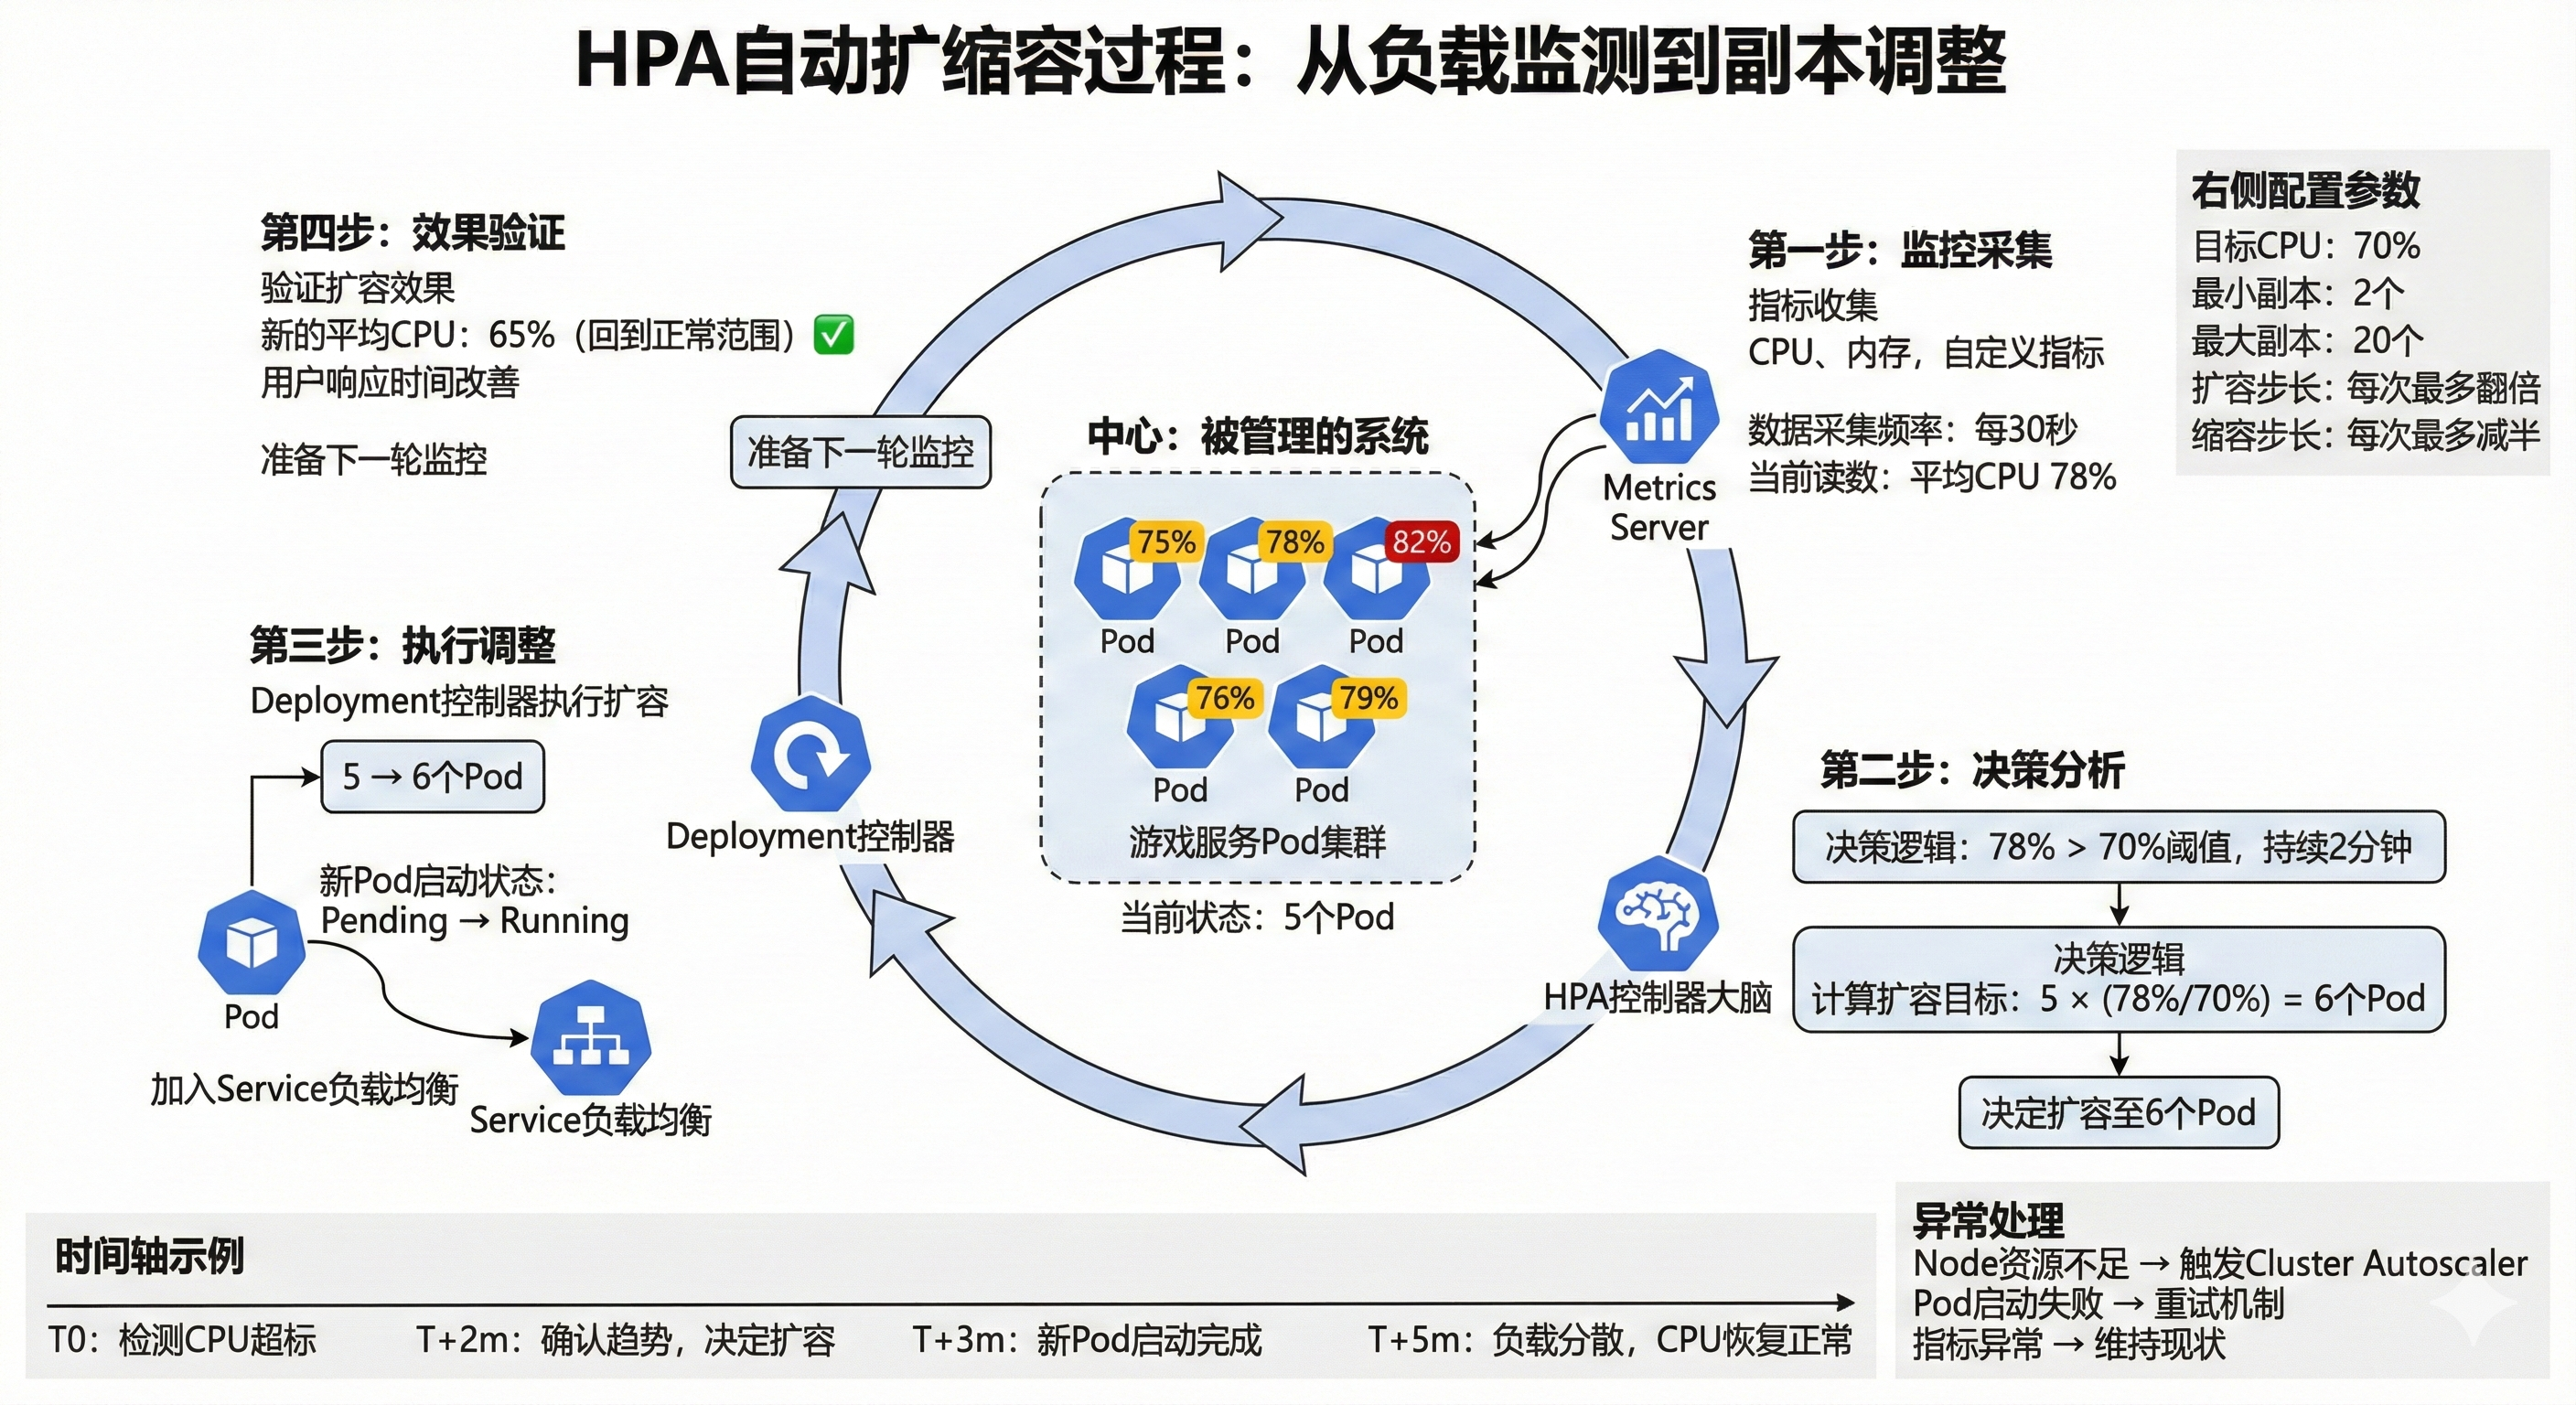
\includegraphics[width=0.9\textwidth]{figures/sec5/hpa-scaling-process.png}
\caption{HPA自动扩缩容过程：从负载监测到副本调整}
\label{fig:hpa-scaling}
\end{figure}

HPA的智能性体现在其多层次的决策机制上。首先是多指标综合评估：不仅仅关注CPU使用率，还会综合考虑内存使用率、网络IO、自定义业务指标等多个维度，避免单一指标可能导致的误判。其次是防抖动机制：通过设置观察窗口期和变化幅度限制，避免因短期波动导致的频繁扩缩容。最后是渐进式调整：每次扩缩容都采用相对温和的步长，给系统足够的时间来响应变化。

在实际的游戏场景中，HPA通常会配置为多阶梯的响应策略。当CPU使用率在60-80\%之间时，属于正常运行区间，不触发任何操作；当超过80\%时，开始扩容，每次增加当前副本数的50\%；当低于30\%且持续一定时间后，开始缩容，每次减少当前副本数的25\%。这种非线性的响应策略既保证了扩容的及时性，又确保了缩容的稳健性。

HPA的配置相对简单，但需要仔细考虑几个关键参数：目标CPU使用率通常设置在70\%左右，既保证了充足的处理能力，又留有应对突发负载的余量；最小副本数确保基本的服务可用性和容错能力；最大副本数防止扩容失控导致成本爆炸；扩缩容的冷却期避免系统震荡。

HPA的真正价值在于它将复杂的容量管理决策自动化了。运维人员不再需要半夜起床处理流量突增，不再需要猜测明天需要多少服务器，不再需要在成本和性能之间做艰难的权衡。只需要设定合理的策略参数，HPA就会7×24小时不间断地监控和调节，确保系统始终运行在最佳状态。

\subsubsection{集群自动扩容：当容器装不下时自动加机器}

当Pod级别的扩容达到Node资源的物理上限时，就需要启动Node级别的扩容，即向集群中添加更多的云服务器。这个过程涉及与云厂商API的深度集成，需要Kubernetes能够自主决定何时购买新服务器、选择什么规格、以及如何将新服务器纳入集群管理。

Cluster Autoscaler（集群自动扩缩器）是实现Node级弹性的核心组件，它的工作原理可以类比为一个智能的办公楼管理系统。当所有现有的办公室都被占满，还有新员工需要入驻时，管理系统会自动租用新的楼层；当某些楼层长期空置时，会将剩余员工集中到其他楼层，然后退租空置楼层以节省成本。

Cluster Autoscaler的触发机制有两个主要场景。扩容触发：当调度器发现有Pod因为资源不足而无法调度到任何现有Node上时，这些Pod会处于Pending状态。Cluster Autoscaler监控到这种情况后，会分析这些Pending Pod的资源需求，然后请求云厂商创建合适规格的新虚拟机实例。新Node启动并加入集群后，调度器就可以将Pending的Pod调度到新Node上运行。

缩容触发相对复杂一些：Cluster Autoscaler会持续监控每个Node的资源利用率，当发现某个Node的利用率长期低于阈值（通常是50\%）时，会评估是否可以将该Node上的所有Pod迁移到其他Node。如果迁移操作不会导致资源不足或违反Pod的调度约束，就会执行Node缩容：首先将该Node标记为不可调度，然后逐个迁移Pod到其他Node，最后将空Node从集群中移除并释放云服务器资源。

Node级扩容的一个关键优势是智能的实例类型选择。现代云厂商通常提供数十种不同规格的虚拟机实例：计算优化型（高CPU核心数）、内存优化型（大内存容量）、存储优化型（高IOPS磁盘）、网络优化型（高带宽）、通用均衡型等。Cluster Autoscaler可以根据Pending Pod的资源需求特征，自动选择最合适且最经济的实例类型。

例如，对于CPU密集型的游戏逻辑计算，Cluster Autoscaler会选择计算优化型实例；对于需要大量缓存数据的Redis服务，会选择内存优化型实例；对于处理大量玩家连接的网关服务，会选择网络优化型实例。这种智能匹配不仅提升了资源利用效率，也避免了"用牛刀杀鸡"式的资源浪费。

\subsubsection{多层弹性：构建真正的自适应系统}

Pod级扩容与Node级扩容的结合，构成了一个完整的多层弹性体系。这种设计体现了现代分布式系统的层次化架构思想：每一层都专注于解决特定范围内的问题，层与层之间通过标准化接口协作，共同实现系统整体的智能行为。

在这个多层体系中，HPA负责应用层的精细化调度。它关注的是Pod级别的资源使用效率，通过增减Pod副本数量来匹配实时负载。HPA的响应速度很快（通常在1-2分钟内），因为它只需要在现有Node上启动或停止容器，不涉及基础设施的变化。

Cluster Autoscaler负责基础设施层的宏观扩展。它关注的是集群整体的资源容量，通过增减Node数量来突破现有集群的资源边界。Cluster Autoscaler的响应速度相对较慢（通常需要3-5分钟），因为它需要与云厂商API交互来创建或销毁虚拟机实例。

\begin{figure}[htbp]
\centering
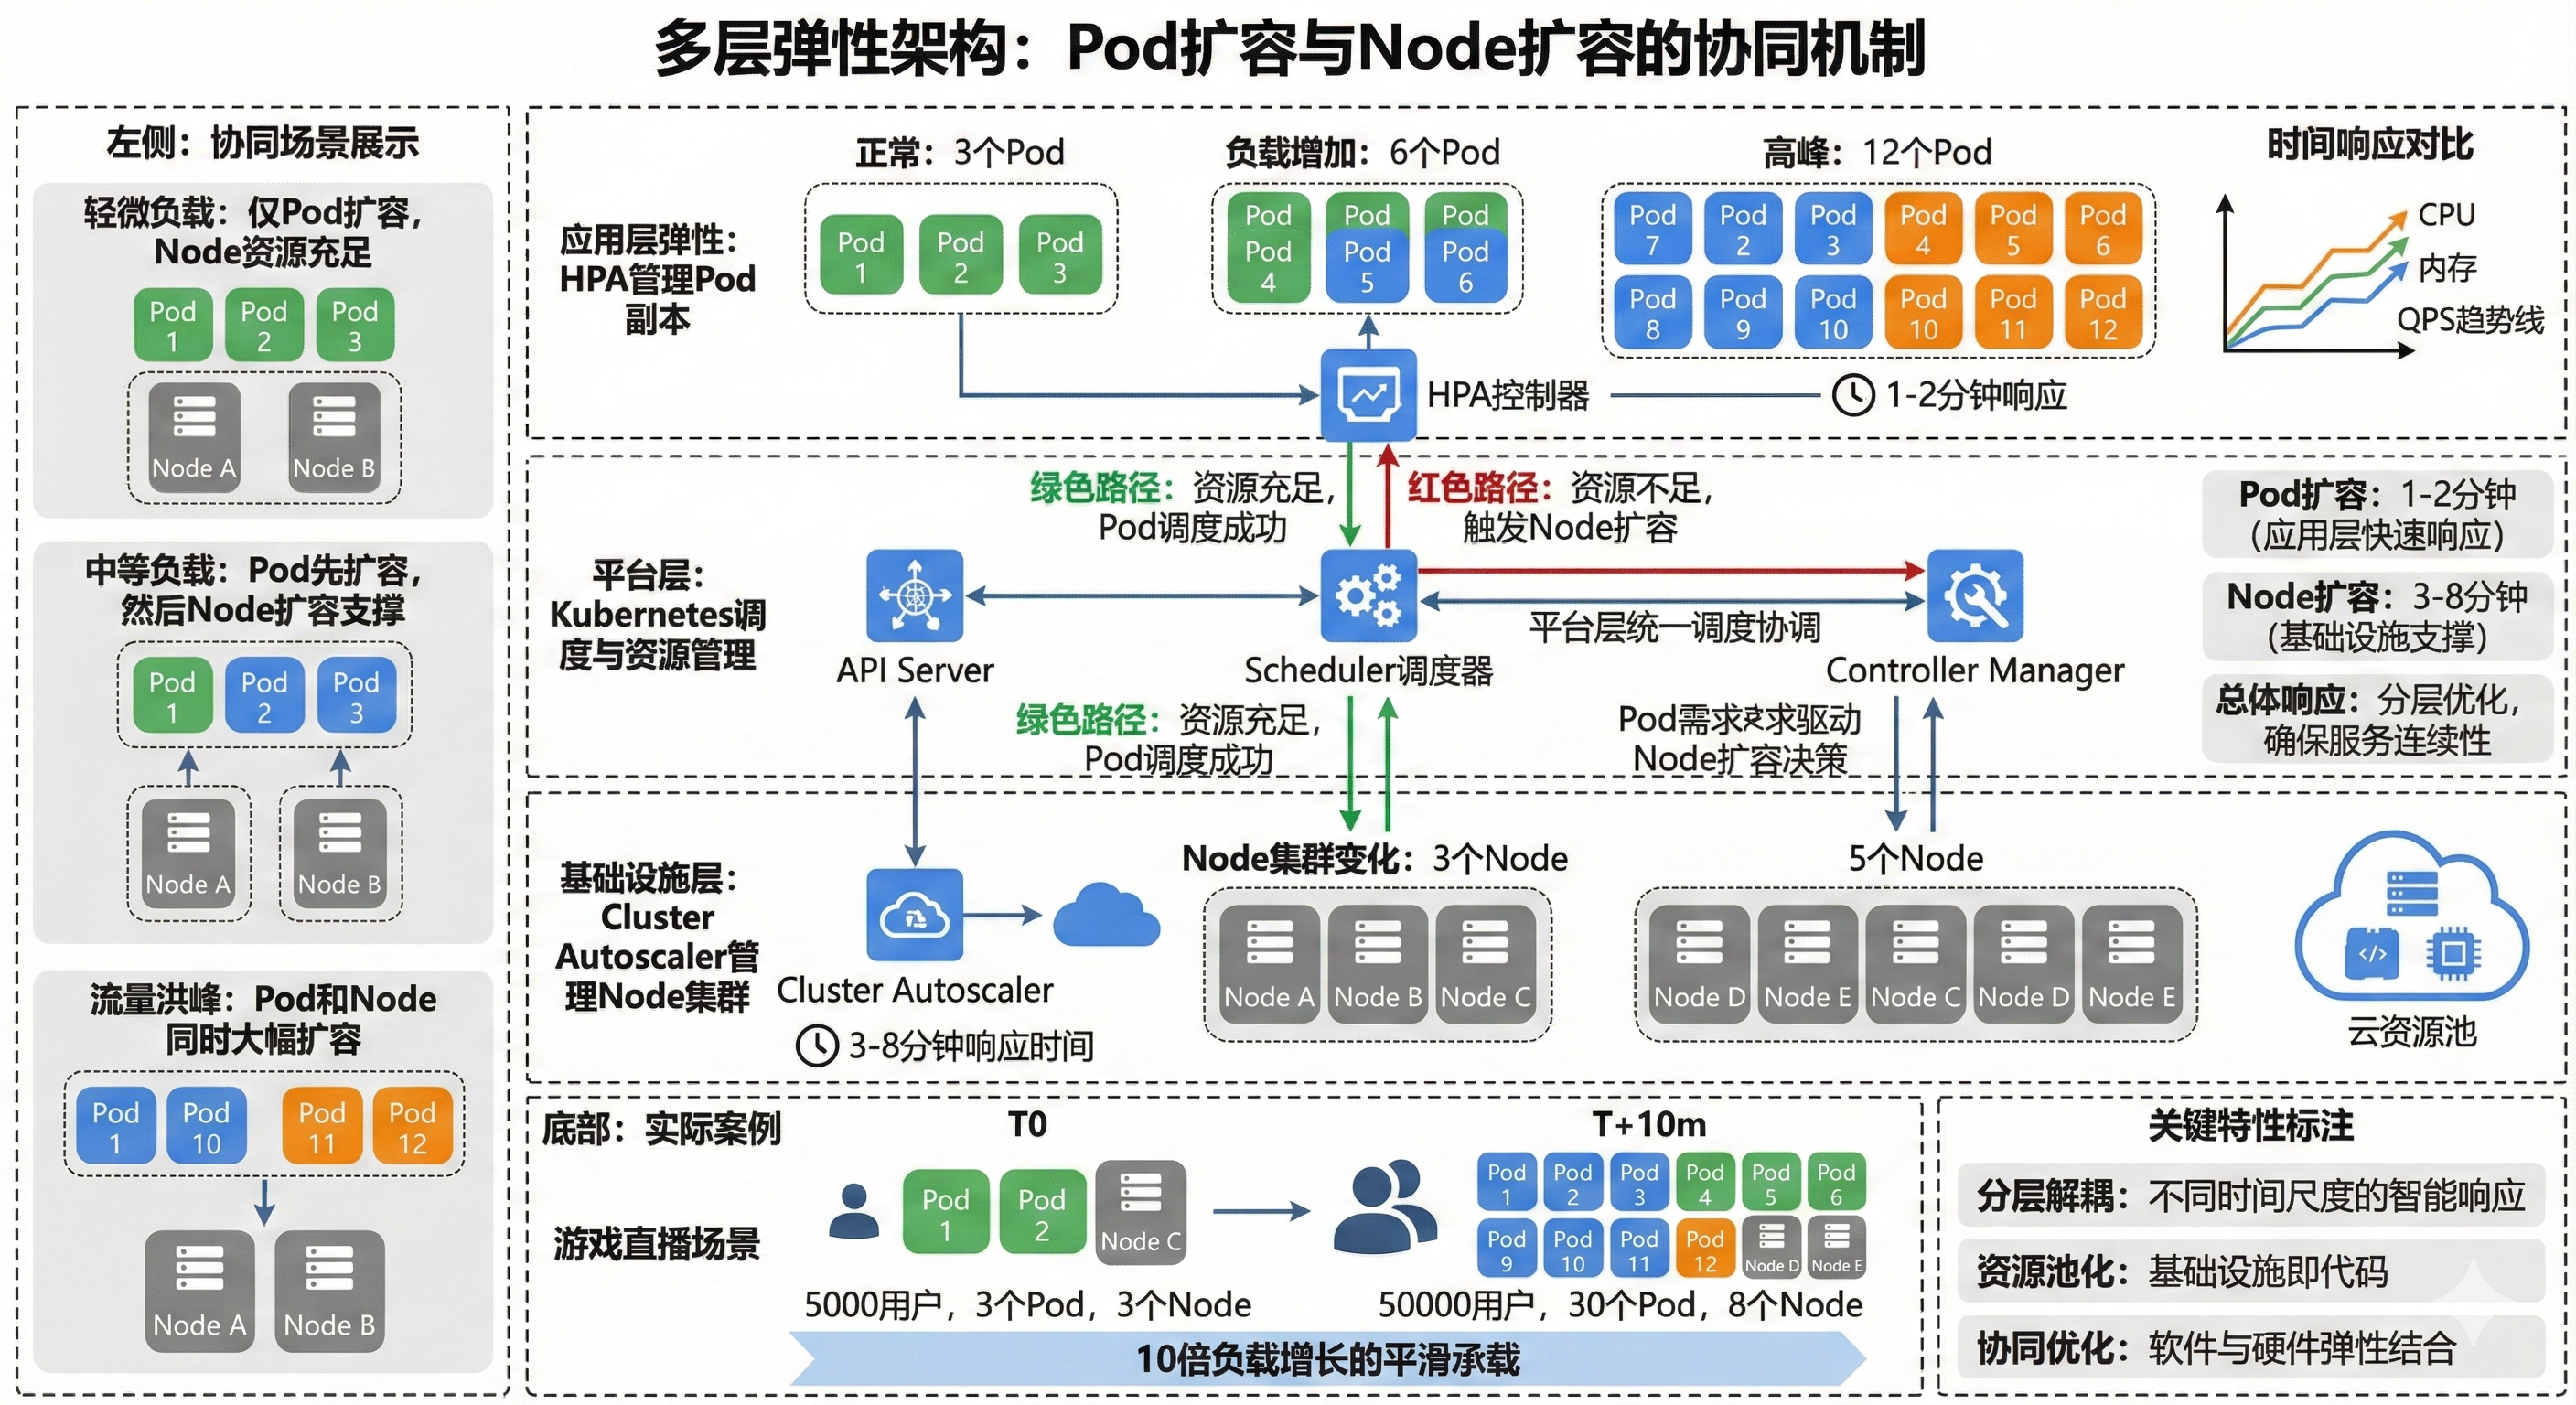
\includegraphics[width=0.9\textwidth]{figures/sec5/multi-layer-elasticity.png}
\caption{多层弹性架构：Pod扩容与Node扩容的协同机制}
\label{fig:multi-layer-elasticity}
\end{figure}

这种分层设计的优势在于它能够处理不同时间尺度和不同强度的负载变化。对于短期的负载波动，HPA能够快速响应，在现有资源范围内进行精细调节；对于长期的容量需求增长，Cluster Autoscaler提供底层支撑，确保有足够的基础资源来承载更多的Pod。两者配合，实现了从秒级到分钟级、从软件层到硬件层的全方位弹性覆盖。

在实际的游戏运营场景中，这种多层弹性的价值尤为明显。比如，某个热门主播开始直播游戏时，观众涌入导致在线人数在10分钟内从5000增长到50000。首先，HPA检测到CPU使用率急剧上升，开始在现有Node上快速增加游戏服务器Pod；当现有Node资源耗尽后，大量新Pod处于Pending状态，触发Cluster Autoscaler开始创建新Node；新Node加入集群后，Pending的Pod被调度到新Node上，整个系统平滑地承载了10倍的负载增长。

更重要的是，当直播结束、在线人数回落后，整个过程会反向进行：HPA首先减少多余的Pod，释放Node上的资源；Cluster Autoscaler发现某些Node利用率过低，开始缩容Node，将剩余Pod重新分布到更少的Node上，然后释放多余的云服务器。这个过程完全自动化，无需任何人工干预，真正实现了"来的时候自动扩，走的时候自动缩"的理想弹性状态。

通过本节的学习，我们不仅掌握了Kubernetes弹性扩容的技术机制，更重要的是理解了现代云原生架构的核心价值：将静态的资源配置转变为动态的策略管理，让系统像生物体一样具备感知环境变化并自适应调节的能力。这种弹性思维的掌握，标志着从传统运维向云原生架构师的重要转变，为构建真正具备互联网级承载能力的系统奠定了坚实基础。

当你看到监控面板上显示"Auto-scaled from 3 to 30 pods in 5 minutes"时，你就真正体验到了云原生弹性的魅力：不是简单的技术优化，而是让系统具备了应对未来不确定性的核心能力。

%\subsection{未来展望：Serverless 架构与无限可能}
%\paragraph{本节目标} 了解 Serverless 概念，掌握其应用场景。
%\paragraph{写作建议}
%\begin{enumerate}
%    \item 对比 K8s：Serverless 不用管服务器，按代码运行时间收费。
%    \item 列适用场景：低频功能（每日签到）、峰值波动功能（节日活动）、轻量逻辑（等级计算）。
%\end{enumerate}



\subsection{未来展望：Serverless架构与无限可能}

\subsubsection{从管理集群到专注业务：Serverless的范式革命}

在我们刚刚掌握的Kubernetes架构中，虽然已经实现了容器编排的自动化和弹性扩容的智能化，但仔细观察会发现，我们依然需要关心许多基础设施层面的细节：Node的规格选择、集群的健康监控、网络的安全配置、存储的持久化策略等等。这些运维工作虽然被K8s大大简化了，但并没有完全消失。对于专注业务创新的开发团队来说，这些"必要但非核心"的技术债务依然会分散精力，影响产品迭代的速度。

Serverless（无服务器）架构的出现，代表了云计算发展的下一个重要阶段：彻底抽象掉服务器管理的复杂性，让开发者只需要关心业务逻辑的实现。这种抽象程度的提升，类似于从汇编语言到高级编程语言的飞跃，或从手动内存管理到自动垃圾回收的进化。每一次抽象层次的提升，都会释放开发者的生产力，让他们能够将更多精力投入到真正创造价值的业务创新上。

在Serverless模式下，你不需要预先购买或配置任何服务器，不需要担心容器的调度和扩缩容策略，甚至不需要关心代码运行在什么操作系统上。你唯一需要做的，就是编写业务逻辑代码，然后将其部署到云厂商的Serverless平台上，平台会自动处理所有的基础设施管理工作。这种"代码即服务"的理念，让基础设施真正变成了不可见的底层支撑。

更具革命性的是，Serverless采用了全新的计费模式：按代码实际运行时间收费，而非按服务器租用时间收费。在传统模式下，即使你的游戏服务器整夜无人访问，你依然需要为那台空转的机器付费；而在Serverless模式下，如果没有玩家触发相关功能，你的代码根本不会运行，自然也不会产生任何费用。这种"用多少付多少"的精确计费，对于具有明显波峰波谷特征的业务场景来说，能够带来显著的成本优势。

\begin{figure}[htbp]
\centering
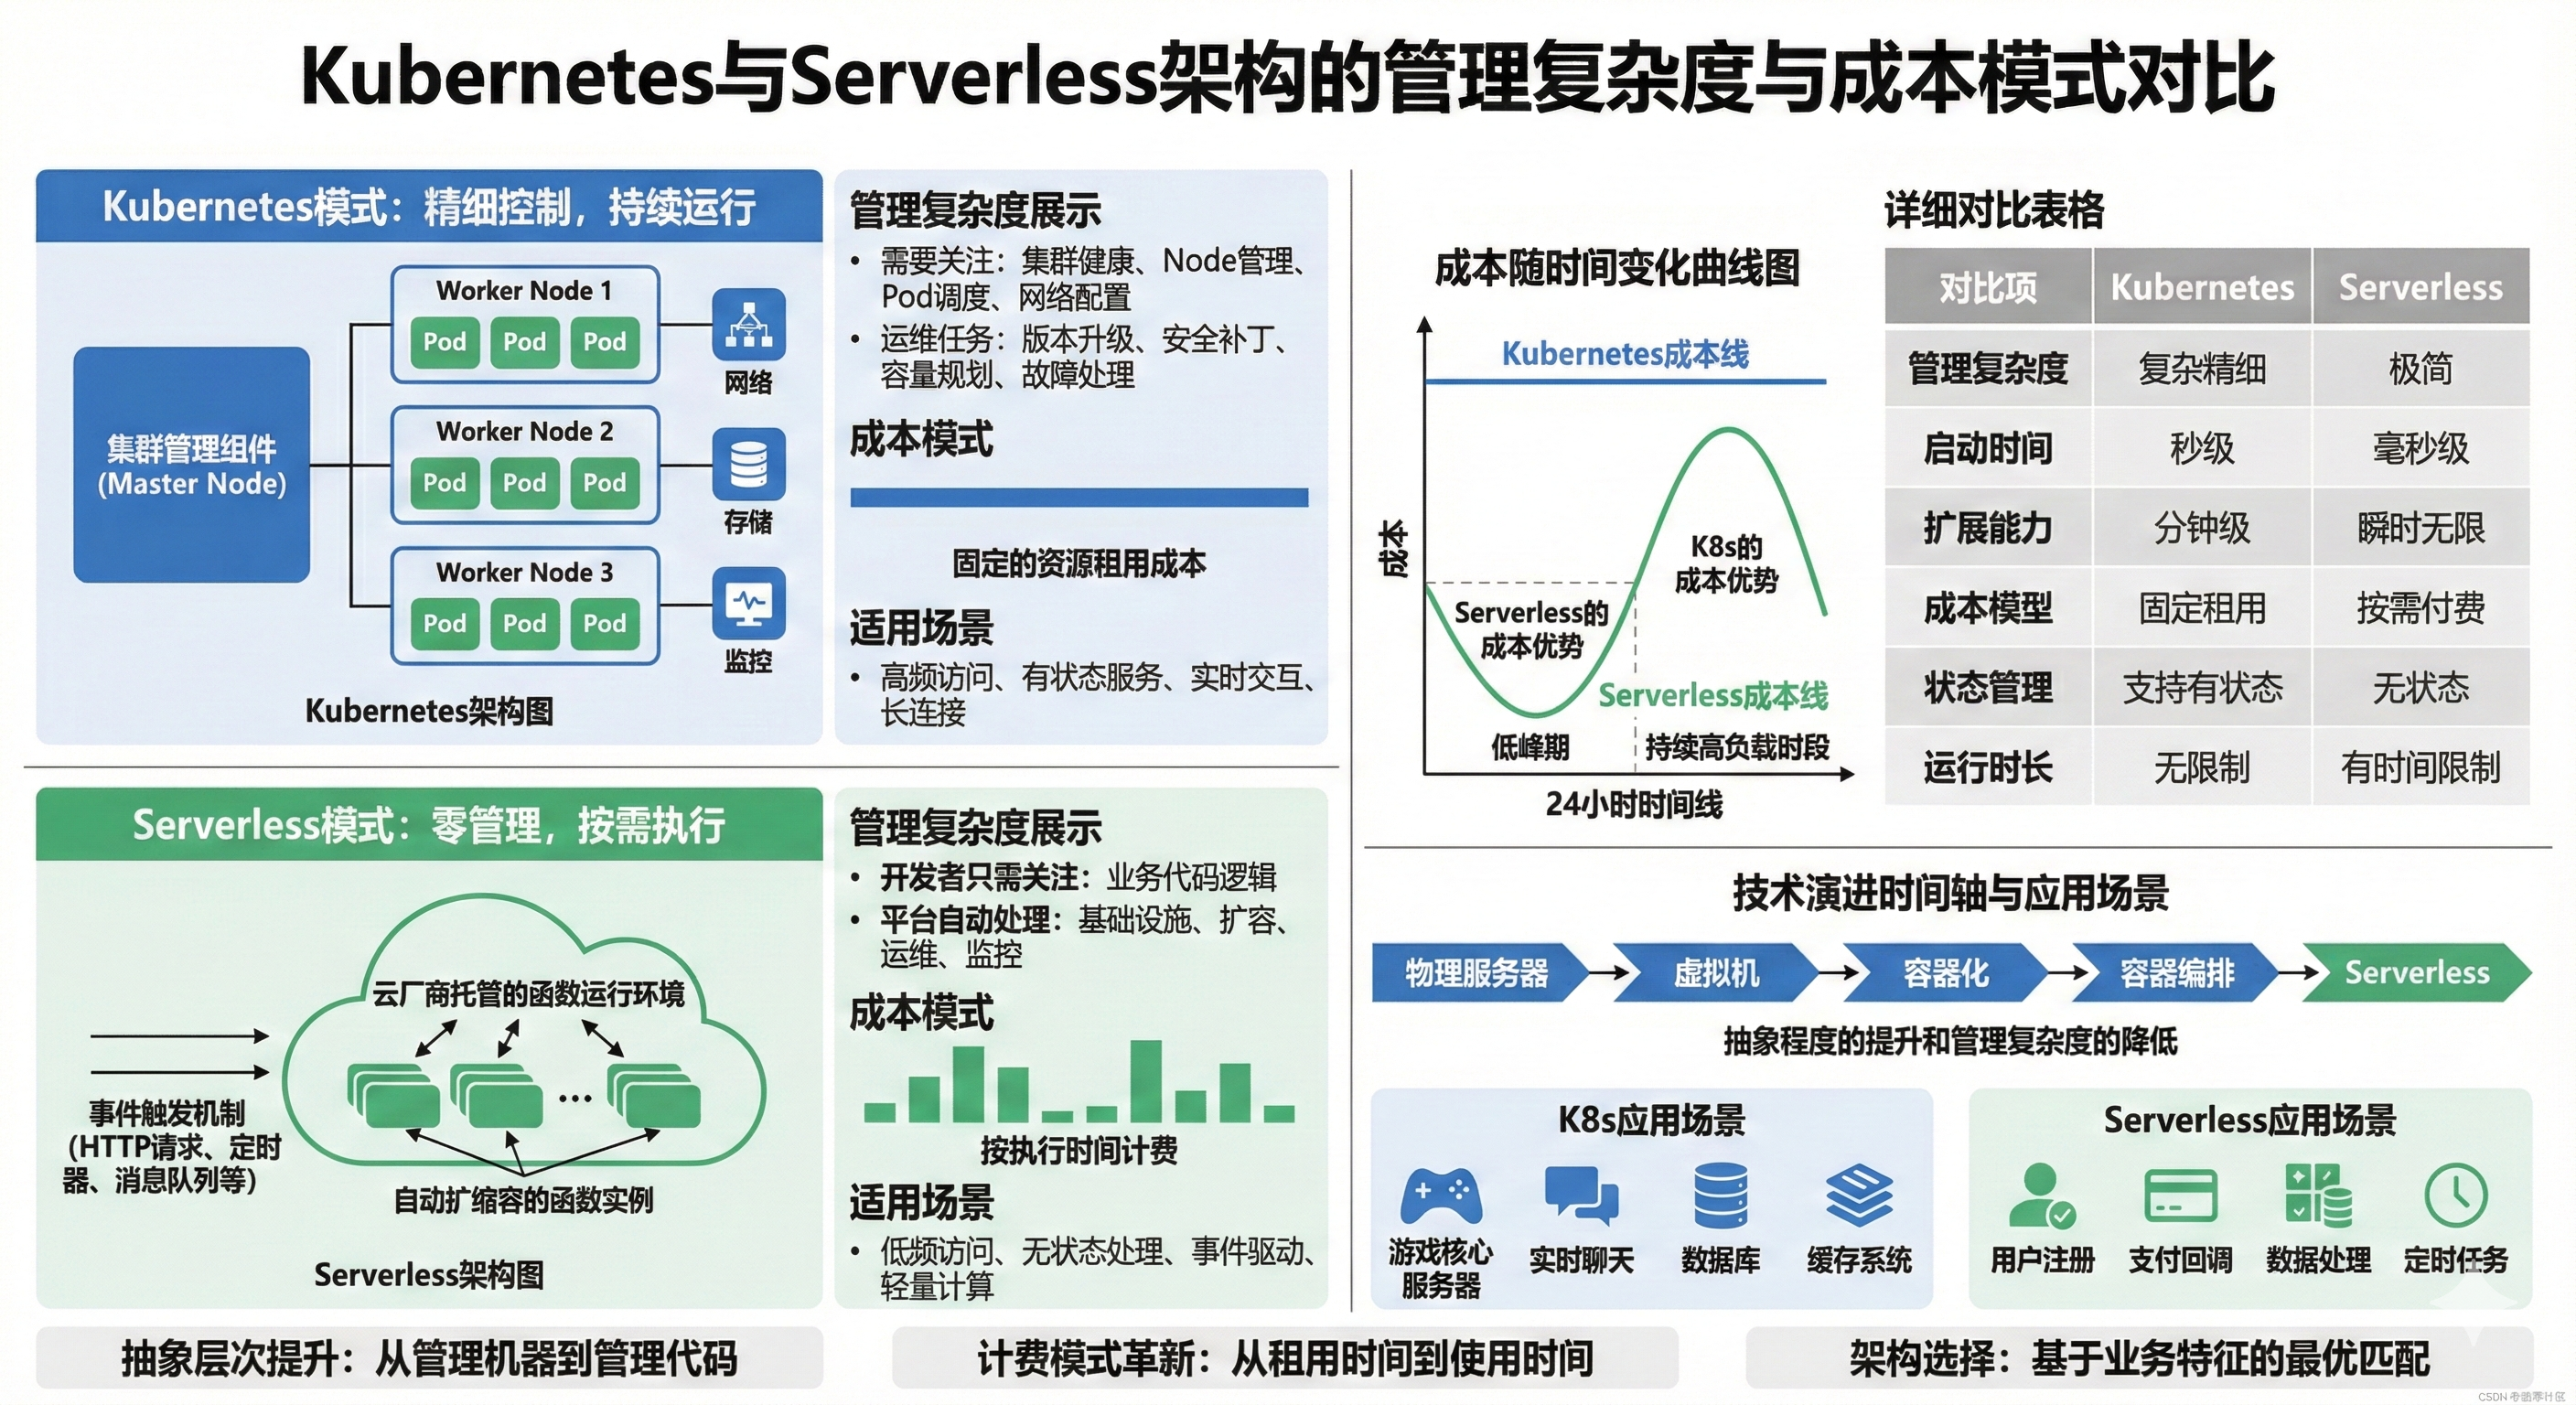
\includegraphics[width=0.9\textwidth]{figures/sec5/kubernetes-vs-serverless-comparison.png}
\caption{Kubernetes与Serverless架构的管理复杂度与成本模式对比}
\label{fig:k8s-vs-serverless}
\end{figure}

如图\ref{fig:k8s-vs-serverless}所示，两种架构模式在管理复杂度、计费方式和适用场景上存在显著差异。Kubernetes提供了更精细的控制能力和更稳定的性能表现，适合作为游戏核心服务的载体；而Serverless则以极简的管理成本和精确的按需付费，在特定业务场景下展现出独特的优势。

Serverless架构的另一个重要特征是事件驱动的执行模型。传统的服务器程序是常驻内存的，持续监听请求并做出响应；而Serverless函数是按需启动的，只在有事件触发时才会执行。这种执行模型非常适合处理不连续的业务逻辑，如用户注册、支付回调、数据同步等。当事件发生时，云平台会在毫秒级时间内启动函数实例处理请求；当处理完成后，实例立即被回收，不占用任何资源。

\subsubsection{游戏场景中的Serverless黄金应用}

虽然Serverless架构具有诸多优势，但并非适用于所有游戏业务场景。它的技术特性决定了其最适合处理低频次、突发性或轻量级的业务逻辑。通过对游戏业务特征的深入分析，我们可以识别出Serverless的几个黄金应用场景。

\textbf{低频功能的完美载体}

每日签到、邮件系统、好友申请处理等功能，虽然是游戏必备的基础模块，但其访问频率相对较低且呈现明显的时间规律性。以每日签到为例，大部分玩家会在每天的固定时间段集中签到，其余22个小时该功能几乎处于空闲状态。如果为此类功能专门维护服务器，将造成严重的资源浪费。

Serverless架构天然适合这种"间歇性高并发"的访问模式。在无人访问时，函数完全不消耗资源和费用；当出现签到高峰时，云平台能够在毫秒级时间内启动成千上万个函数实例，自动应对并发压力。更重要的是，这类功能通常不需要维持复杂的状态，单次请求可以独立处理，非常契合Serverless的无状态特性。

\textbf{突发流量的弹性缓冲器}

游戏运营中经常会遇到不可预测的突发流量：新版本发布、网红主播推荐、突发热点事件等都可能在短时间内带来数十倍的访问量增长。传统架构需要提前预估峰值并预留资源，但预估往往不准确，要么资源不足导致服务崩溃，要么过度预留造成浪费。

Serverless提供了理论上无限的并发扩展能力，能够自动应对任何规模的突发流量。当流量洪峰到来时，云平台会根据实际请求量动态启动函数实例；当流量回落时，多余的实例自动销毁。这种"用时即启动，完毕即销毁"的执行模式，让系统具备了应对"黑天鹅事件"的能力，而无需为极端情况买单。

节日活动、限时副本、抢购活动等具有明显时效性的功能，特别适合采用Serverless架构。活动期间可以获得充足的计算资源，活动结束后立即停止资源消耗，实现了真正的按需使用。

\begin{figure}[htbp]
\centering
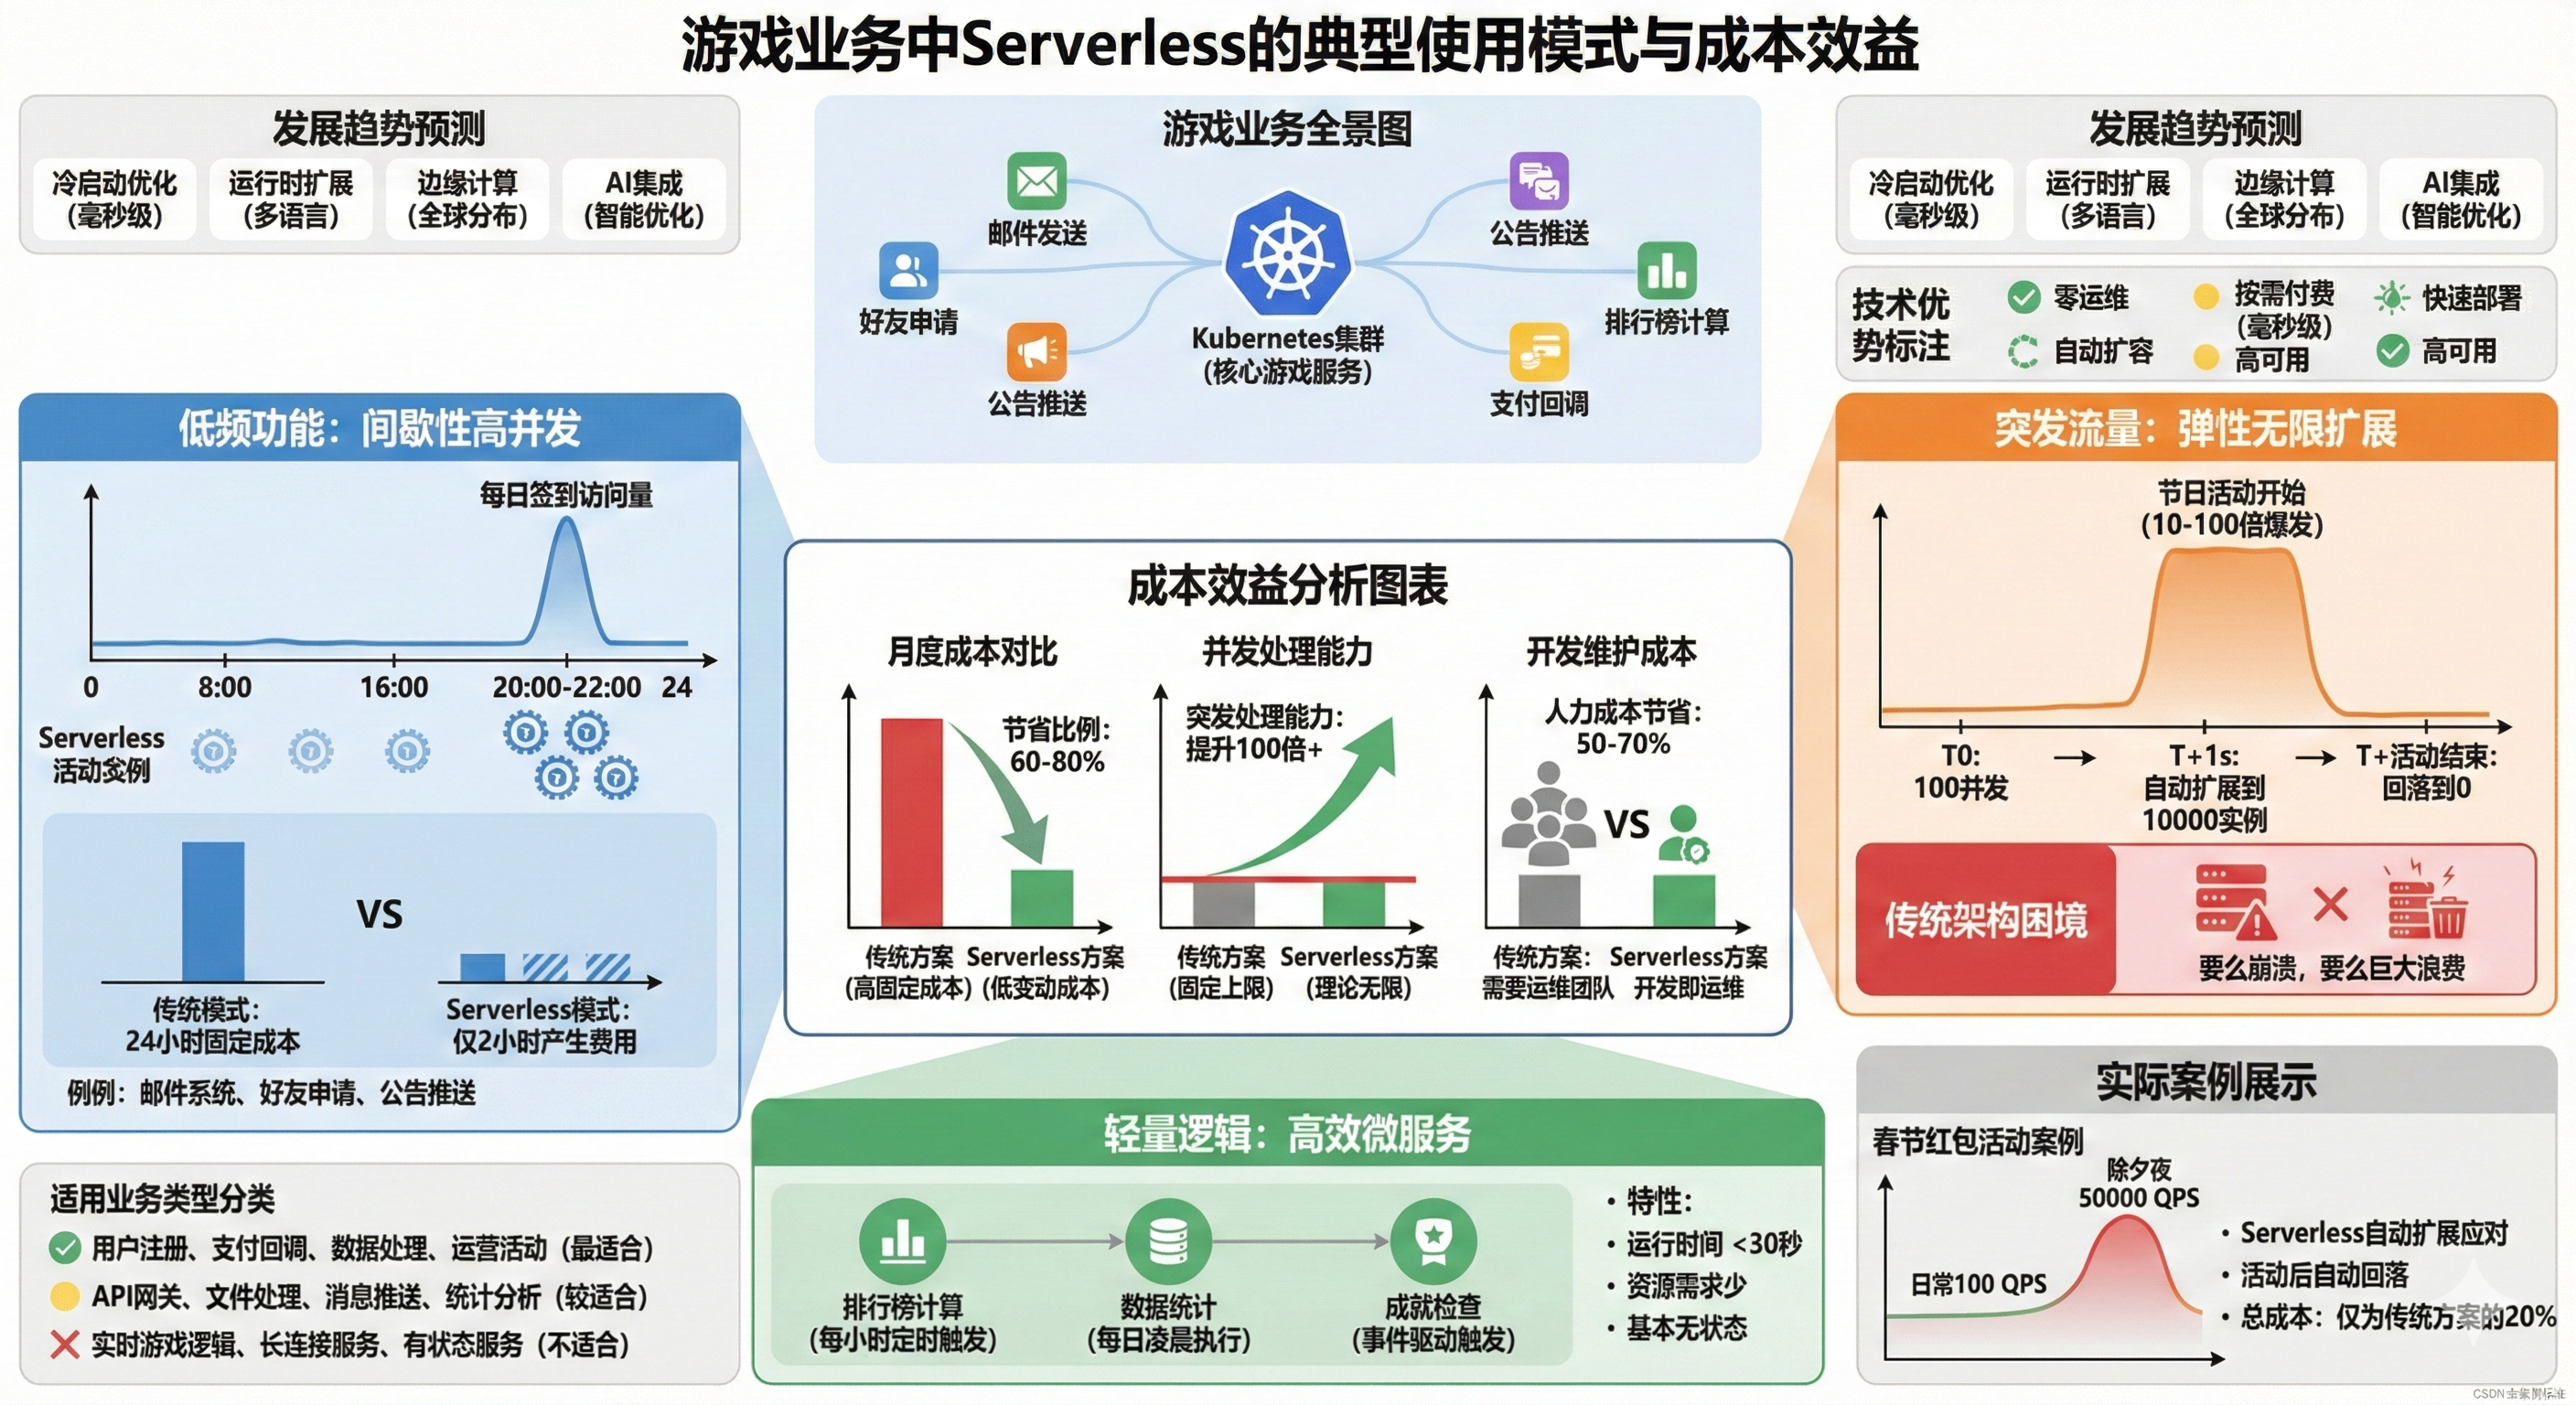
\includegraphics[width=0.9\textwidth]{figures/sec5/serverless-usage-patterns.png}
\caption{游戏业务中Serverless的典型使用模式与成本效益}
\label{fig:serverless-patterns}
\end{figure}

\textbf{轻量逻辑的高效执行器}

游戏中存在大量轻量级的计算任务：排行榜更新、成就进度检查、每日任务重置、数据统计分析等。这些任务通常逻辑简单、执行时间短暂、不需要复杂的资源管理，但又是游戏运营不可缺少的重要环节。

Serverless函数非常适合承载这类轻量级任务。函数的冷启动时间已经优化到百毫秒级别，对于大多数计算任务来说完全可以接受。而且，这类任务往往可以设计为定时触发或事件驱动，与Serverless的执行模型天然匹配。

例如，排行榜计算可以设计为每小时定时触发的Serverless函数，从数据库读取玩家数据，进行排序计算，然后将结果写入缓存。整个过程只需要几秒钟的执行时间，但如果用传统方式部署专门的服务器，就需要7×24小时运行以等待这每小时一次的任务执行。

\subsubsection{架构融合：构建最优的混合云策略}

在实际的游戏项目中，Serverless并不是要完全替代Kubernetes，而是与其形成优势互补的混合架构。这种架构选择的核心原则是：让合适的技术处理合适的场景，实现整体系统的最优性价比。

核心游戏服务（如实时对战、世界状态同步、聊天系统）需要维持长连接、处理高频交互、管理复杂状态，这类服务依然适合运行在Kubernetes集群上。K8s提供的精细资源控制、网络管理、存储编排等能力，能够保证核心服务的稳定性和性能。

而周边的辅助功能（如用户注册、支付回调、数据分析、运营活动）则可以逐步迁移到Serverless平台，实现成本优化和运维简化。这些功能通常具有无状态、低频次、可独立执行的特点，正好契合Serverless的技术优势。

\begin{figure}[htbp]
\centering
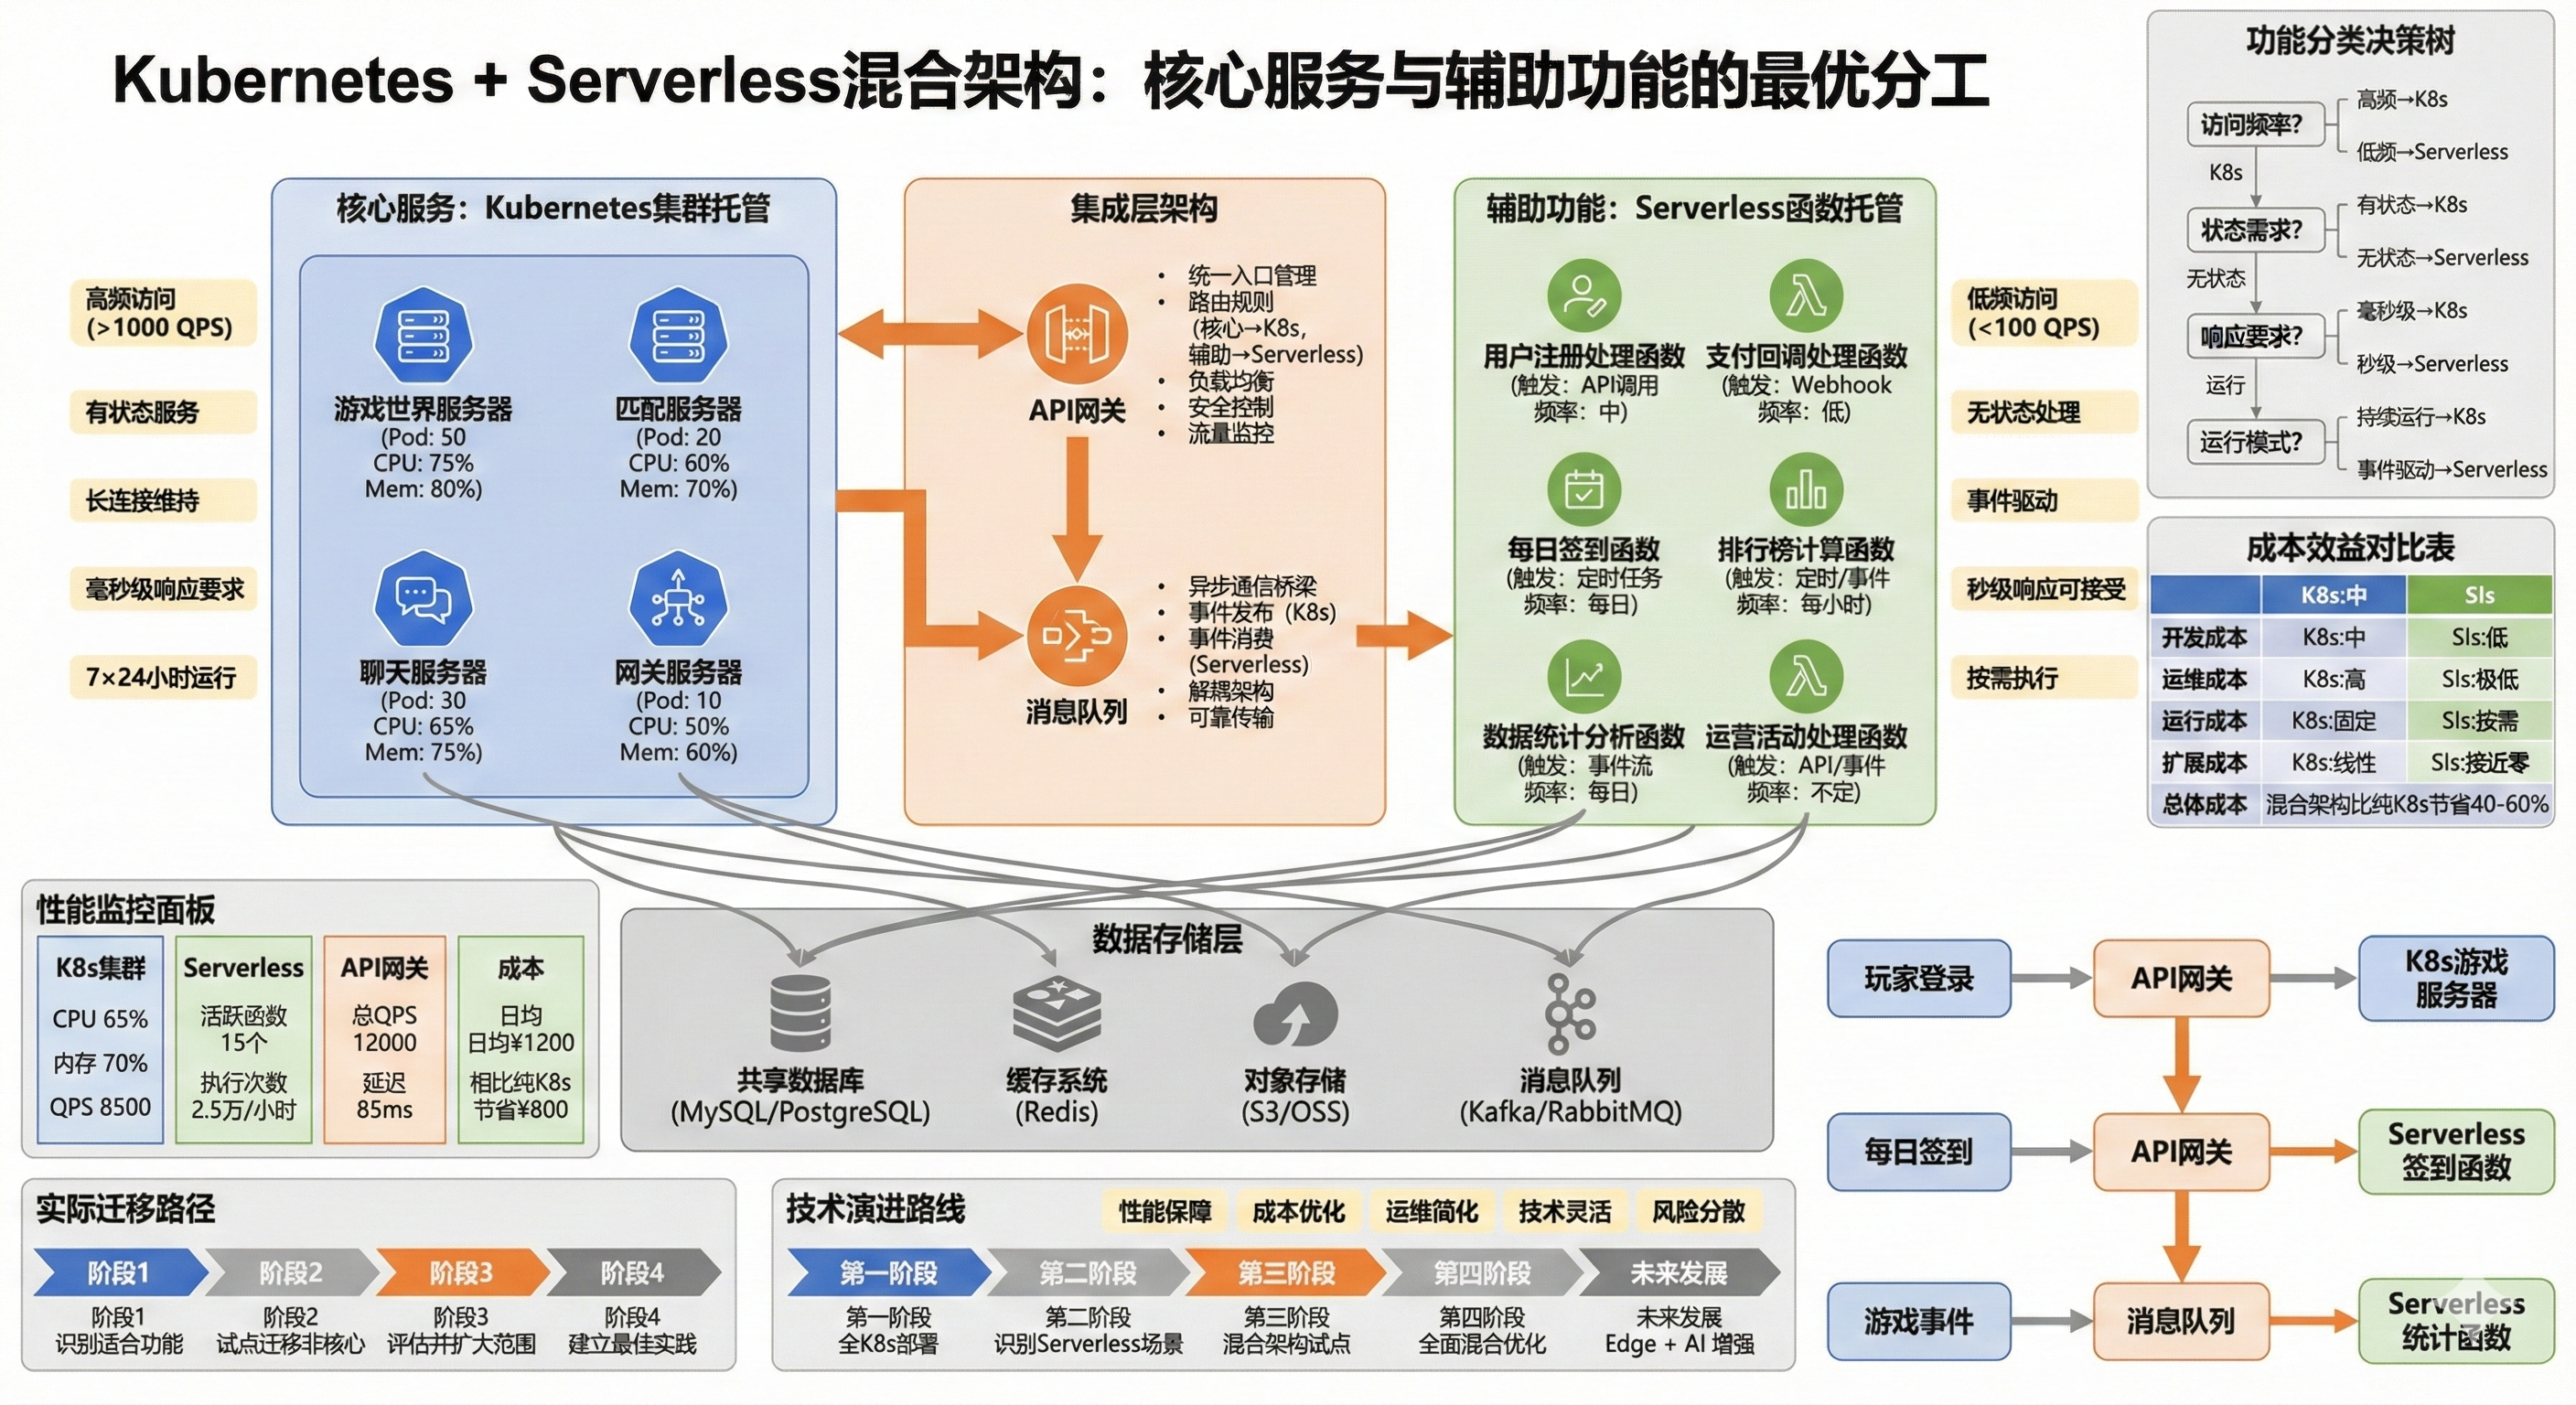
\includegraphics[width=0.9\textwidth]{figures/sec5/hybrid-architecture-design.png}
\caption{Kubernetes + Serverless混合架构：核心服务与辅助功能的最优分工}
\label{fig:hybrid-architecture}
\end{figure}

如图\ref{fig:hybrid-architecture}所示，混合架构通过合理的功能分层，既保证了游戏核心体验的稳定性，又充分利用了Serverless在成本和运维方面的优势。两种架构通过API网关、消息队列、共享数据库等方式实现无缝集成，形成统一的技术生态。

这种混合策略的实施可以采用渐进式迁移的方式：首先识别系统中适合Serverless的功能模块，评估迁移的技术可行性和商业价值；然后逐个模块进行迁移试点，积累经验和最佳实践；最后基于试点效果决定进一步的迁移范围。这种approach既能够快速获得Serverless的收益，又能够将迁移风险控制在可接受范围内。

\subsubsection{技术展望：Serverless的未来演进}

随着云厂商对Serverless技术的持续投入和优化，其技术能力边界正在不断扩展。冷启动时间从秒级优化到毫秒级，执行环境从简单脚本扩展到完整应用，触发方式从HTTP请求扩展到数十种事件源，运行时长从几分钟扩展到几小时。这些技术进步让Serverless能够承载越来越复杂的业务场景。

特别值得关注的是边缘计算与Serverless的结合。云厂商正在将Serverless计算能力部署到全球各地的边缘节点，让函数能够在离用户更近的位置执行。这种Edge Serverless架构对于游戏业务具有特殊意义：可以显著降低网络延迟，提升玩家体验；可以就近处理地域性的业务逻辑，减少数据传输成本；可以更好地支持全球化运营，适应不同地区的监管要求。

另一个重要的发展方向是Serverless与AI/ML的深度集成。云平台正在提供越来越多的预训练AI模型和机器学习服务，这些服务可以通过Serverless函数轻松调用。对于游戏业务来说，这意味着可以用极低的成本构建智能化功能：智能客服、内容审核、个性化推荐、作弊检测等，而无需投入大量资源来构建和维护AI基础设施。

可以预见，未来一个理想的游戏后端架构将是这样的：Kubernetes集群承载核心的游戏世界，提供稳定的实时交互能力；Serverless函数处理所有的辅助功能，提供极致的成本效率；Edge Computing将部分逻辑推送到用户附近，提供最优的响应体验；AI Services提供智能化的增值功能，提升产品竞争力。这四大技术栈相互协作，共同构建一个既高性能又低成本、既稳定可靠又灵活敏捷的云原生游戏生态。

通过本章的学习，我们完成了从本地开发到云端部署的完整技术栈掌握：Docker容器化解决了环境一致性问题，Kubernetes提供了工业级的编排能力，弹性扩容实现了资源的智能调度，而Serverless则为特定场景提供了更优的解决方案。这套完整的云原生技术体系，将为你构建下一代游戏产品提供坚实的技术底座。

当你能够灵活运用这些技术，根据业务特点选择最适合的架构模式时，你就真正掌握了云原生时代的核心竞争力：不是简单地使用某种技术，而是基于深度理解来设计最优的技术组合，让技术真正服务于业务价值的创造。


\subsubsection{小结：从“本地原型”到“云原生工业”}

本章的旅程，实质上是一场对软件交付模式的工业化革命。在章节之初，我们还困在“本地原型”的局限中，依赖开发者的个人电脑和手工配置，像呵护盆栽一样小心翼翼地维护着单体服务。而通过引入 Docker，我们首先解决了“标准化零件”的问题，让代码与其运行环境彻底解耦，实现了“一次构建，处处运行”的交付契约。

随后，我们通过 Kubernetes 建立了一套自动化的“生产流水线”。在这个阶段，我们不再关注单台服务器的死活，而是站在“集群指挥官”的视角，用声明式的配置驾驭成百上千的容器实例。我们将资源的调度权交给了算法，将故障的修复权交给了系统，让游戏世界具备了自我修复和自我进化的能力。

最后，通过弹性伸缩与 Serverless 的探索，我们触碰到了云原生的终极形态：让算力像水电一样“即开即用”。至此，我们的游戏架构彻底摆脱了物理硬件的重力束缚，从一个脆弱的本地原型，进化为一座能够根据流量潮汐自由呼吸、永续运行的“云原生工业堡垒”。

这不仅是技术概念的层层递进式学习，更是系统工程思维维度的跃升。当我们将基础设施代码化、自动化之后，我们终于可以从繁琐的运维泥潭中抽身，将精力回归到最本质的创造，为玩家编织更宏大的游戏世界。

\newpage